\documentclass[11pt,a4paper]{article}
\usepackage[margin=2.3cm]{geometry}
\usepackage{booktabs}
\usepackage{array}
\usepackage{xcolor}
\usepackage{longtable}
\usepackage{enumitem}
\usepackage{xurl}
\usepackage{amsmath}
\usepackage{graphicx}
\usepackage{caption}
\definecolor{ink}{HTML}{0B0B0B}
\definecolor{muted}{HTML}{52514E}
\definecolor{rule}{HTML}{C9C7C2}
\definecolor{accent}{HTML}{57068C}
\definecolor{panel}{HTML}{F4F2EE}
\definecolor{good}{HTML}{14663C}

\usepackage[hidelinks,colorlinks=true,linkcolor=accent!75!black,urlcolor=blue!60!black,citecolor=black]{hyperref}
\usepackage{titlesec}
\usepackage{fancyhdr}

\titleformat{\section}{\large\bfseries\color{accent}}{\thesection}{0.7em}{}
\titleformat{\subsection}{\normalsize\bfseries}{\thesubsection}{0.6em}{}
\titleformat{\subsubsection}{\small\bfseries}{\thesubsubsection}{0.5em}{}
\setlist[itemize]{leftmargin=1.2em,itemsep=2pt,topsep=3pt}
\setlist[enumerate]{leftmargin=1.4em,itemsep=2pt,topsep=3pt}
\renewcommand{\arraystretch}{1.25}

\pagestyle{fancy}\fancyhf{}
\fancyhead[L]{\footnotesize\color{muted}Weekend Margin Clearinghouse — Final Report}
\fancyhead[R]{\footnotesize\color{muted}Team 9}
\fancyfoot[C]{\footnotesize\color{muted}\thepage}
\renewcommand{\headrulewidth}{0.4pt}

\captionsetup{font=small,labelfont={bf,color=accent}}

% pack figures more densely instead of one per mostly-empty float page
\renewcommand{\topfraction}{0.92}
\renewcommand{\bottomfraction}{0.75}
\renewcommand{\textfraction}{0.06}
\renewcommand{\floatpagefraction}{0.80}
\setcounter{topnumber}{3}
\setcounter{totalnumber}{4}

\newcommand{\note}[1]{{\small\color{muted}#1}}
\newcommand{\cbox}[1]{%
  \begin{center}\colorbox{panel}{\parbox{0.95\textwidth}{\vspace{3pt}#1\vspace{3pt}}}\end{center}}
\newcommand{\etx}[1]{{\footnotesize\href{https://sepolia.etherscan.io/tx/#1}{\nolinkurl{#1}}}}
\newcommand{\ead}[1]{{\footnotesize\href{https://sepolia.etherscan.io/address/#1}{\nolinkurl{#1}}}}
\newcommand{\eshort}[2]{\href{https://sepolia.etherscan.io/tx/#1}{#2}}
% Block, time, BTC price and Fund A's live state at the reconciliation read, written by recon_table.py.
% Generated by recon_table.py from the notebook's reconciliation read. Do not edit by hand.
\newcommand{\reconBlock}{12,052,818}
\newcommand{\reconTime}{2026-11-03 04:09 UTC}
\newcommand{\reconBtc}{76,816.82}
\newcommand{\reconCount}{28}
\newcommand{\reconCategoryTable}{%
\begin{tabular}{@{}p{7.2cm}rp{5.4cm}@{}}
\toprule
\textbf{Read at block \reconBlock, \reconTime} & \textbf{Compared} & \textbf{Result} \\
\midrule
Settlements (amount due and funding) & 8 & all match \\
Vault purchase (price and sBILL taken) & 2 & all match \\
Vault redemption (cash received and profit) & 2 & all match \\
sBILL redeemed with the fund (tUSDC paid) & 1 & match \\
sBILL subscriptions (NAV and shares minted) & 4 & all match \\
Live state (NAV, purchase price, funding total) & 4 & all match \\
Account health (collateral, equity, both margin levels) & 4 & all match \\
Unrealized P\&L, both sides of trade 1 & 2 & all match \\
Liquidation reward, stress set & 1 & match \\
\midrule
\textbf{Total} & \textbf{28} & \textbf{28 match, difference 0} \\
\bottomrule
\end{tabular}}
\newcommand{\liveLongPnlSigned}{-\$1{,}646.734697511218543664}
\newcommand{\liveShortPnlSigned}{+\$1{,}646.734697511218543664}
\newcommand{\liveMarginValue}{29{,}270.340627669335719301}
\newcommand{\liveEquity}{30{,}917.075325180554262965}
\newcommand{\liveMaintenance}{7{,}681.682265454000000000}
\newcommand{\liveInitial}{15{,}363.364530908000000000}
\newcommand{\liveEquityRounded}{30{,}917}
\newcommand{\liveMaintenanceRounded}{7{,}682}

% The stress-weekend table of Section 4, written by stress_weekends.py.
% Generated by stress_weekends.py from docs/data/btc_usd_1h_coinbase.csv. Do not edit by hand.
\newcommand{\stressVaultNinetyFive}{98{,}461}
\newcommand{\stressTypicalPct}{3.95\%}
\newcommand{\stressExceed}{four}
\newcommand{\stressTable}{\setlength{\tabcolsep}{4pt}%
\begin{tabular}{@{}p{3.6cm}p{1.8cm}rrrr>{\raggedright\arraybackslash}p{1.7cm}@{}}
\toprule
\textbf{Regime} & \textbf{Weekend} & \textbf{BTC Fri 4pm} & \textbf{Excursion} & \textbf{Loser} & \textbf{Sold per \$1m} & \textbf{\% of 95th-pct vault} \\
\midrule
Yen carry unwind & 2024-08-02 & \$62{,}558 & 20.41\% & long & \$204{,}111 & \textbf{207\%} \\
June 2022 CPI shock & 2022-06-10 & \$28{,}951 & 18.33\% & long & \$183{,}343 & \textbf{186\%} \\
SVB / USDC depeg & 2023-03-10 & \$19{,}975 & 13.51\% & short & \$135{,}125 & \textbf{137\%} \\
May 2021 mining ban & 2021-05-14 & \$50{,}165 & 14.44\% & long & \$144{,}379 & \textbf{147\%} \\
LUNA/UST collapse & 2022-05-06 & \$35{,}996 & 8.86\% & long & \$88{,}640 & 90\% \\
Oct 2025 liquidations & 2025-10-10 & \$116{,}673 & 5.92\% & long & \$59{,}211 & 60\% \\
FTX collapse & 2022-11-11 & \$16{,}573 & 4.44\% & long & \$44{,}435 & 45\% \\
\midrule
Typical weekend & --- & --- & 3.95\% & --- & \$39{,}472 & 40\% \\
\bottomrule
\end{tabular}}



\begin{document}

%====================== TITLE ======================
\thispagestyle{empty}
\vspace*{1.2cm}
\begin{center}
{\footnotesize\color{muted}NYU TANDON SCHOOL OF ENGINEERING \quad·\quad FINANCE \& RISK ENGINEERING}\\[18pt]
{\Huge\bfseries\color{accent} Weekend Margin}\\[10pt]
{\LARGE\bfseries Clearinghouse}\\[16pt]
\rule{0.55\textwidth}{0.8pt}\\[14pt]
{\large An on-chain clearinghouse for Bitcoin perpetual swaps that takes\\ tokenized T-bills as margin and still pays winners on a Saturday}\\[22pt]
{\normalsize FRE-GY 6931 Blockchain \& Cryptocurrency \quad·\quad Fall 2026 \quad·\quad \textbf{Team 9}}\\[10pt]
\begin{tabular}{@{}ll@{}}
Sai Kishore \; (\texttt{sp8744}) & contracts, deployment, front end\\
Swastik Mishra \; (\texttt{sgm9198}) & financial analysis, product, going to market\\
\end{tabular}\\[14pt]
{\small Prof.\ Richard Radnay \quad·\quad TA Hina Tomar \quad·\quad \today}\\[20pt]
\colorbox{panel}{\parbox{0.86\textwidth}{\vspace{4pt}
\small
\begin{tabular}{@{}p{3.1cm}p{10.4cm}@{}}
\textbf{Topic} & 2 — Hedging with perpetual swaps \\
\textbf{Network} & Ethereum Sepolia \\
\textbf{Our token} & \textbf{sBILL} — Tokenized T-Bill Share (ERC-20), \ead{0x2aff94631070707436ef712c4a6e77ecaf4c6720} \\
\textbf{Contracts} & 16 deployed, \textbf{16 verified on Etherscan} \\
\textbf{Repository} & \url{https://github.com/Psaikishore/WeekendMarginDemo} \quad tag \texttt{final} \\
\textbf{Evidence} & \texttt{submission.json} in the repository root \\
\end{tabular}\vspace{4pt}}}
\end{center}

\vfill
\note{\centering Every token in this project is a test token with no value. Nothing here is investment advice.\par}
\clearpage

%====================== DELIVERABLES MAP ======================
\section*{Where to find everything}
\addcontentsline{toc}{section}{Where to find everything}

The brief lists six deliverables. The table below says where each one is.

\begin{center}
\small
\begin{tabular}{@{}p{0.6cm}p{4.6cm}p{10.6cm}@{}}
\toprule
\textbf{\#} & \textbf{Deliverable} & \textbf{Where it is} \\
\midrule
1 & Contracts on Sepolia, including our token, verified on Etherscan & All 16 addresses in \textbf{Section~\ref{sec:addresses}}; verification and metadata in \S\ref{sec:metadata}; Etherscan screenshots in \S\ref{sec:evidence}; every function tabulated in \S\ref{sec:arch} \\
2 & GitHub repository, tagged \texttt{final}, with a README & \url{https://github.com/Psaikishore/WeekendMarginDemo}; the README explains what the project does and how to run the tests \\
3 & \texttt{submission.json} & Repository root; its structure is in \textbf{Appendix~\ref{app:json}}; the eight key transactions are in \textbf{Appendix~\ref{app:addresses}} \\
4 & Report (PDF) under the eight required headings & This document, \texttt{docs/report.pdf} \\
5 & Financial analysis in \texttt{docs/} & \texttt{docs/analysis.ipynb}, summarised with its charts in \textbf{Section~\ref{sec:finance}}; the business case is \textbf{Section~\ref{sec:gtm}} \\
6 & Video: narrated, every member speaks, at least one live Sepolia transaction & Linked in \texttt{submission.json}; the running application is described in \S\ref{sec:frontend} \\
\bottomrule
\end{tabular}
\end{center}

\begin{center}
\small
\begin{tabular}{@{}p{4.3cm}p{11.5cm}@{}}
\toprule
\textbf{Graded area} & \textbf{Our answer, in one line} \\
\midrule
I. Rigor of methodology & Every input declared in one config file; 28 model values reconciled to the wei against the live contracts (\S\ref{sec:reconcile}); break points located for each assumption (\S\ref{sec:breaks}). \\
II. Design decisions & 18 decisions, each with the alternative we considered and the reason; 5 of them changed during the build because of a measurement (\S\ref{sec:design}). \\
III. Scope delivered & 6 contracts in 3 labelled deployment sets, 37 tests, keeper, 7-page front end, one-command on-chain run, notebook, 3 documents. All live (\S\ref{sec:arch}, \S\ref{sec:liverun}). \\
IV. Presentation and going to market & This report with contents and screenshots; a go-to-market plan with a break-even number and a named reason the product cannot ship on mainnet (\S\ref{sec:gtm}). \\
V. Quality of code & OpenZeppelin throughout, packed storage, custom errors, \texttt{nonReentrant} on every entry point, Slither scanned and every finding answered (\S\ref{sec:testing}). \\
VI. Advanced functionality & Nine features, each with a transaction hash or a file (\S\ref{sec:advanced}). \\
\bottomrule
\end{tabular}
\end{center}

\vspace{6pt}
\cbox{\textbf{The one-sentence version.} A fund can keep its money in Treasury bills, earning
interest, and still pay what it owes on a Sunday — because when the T-bill
market is shut, a permissionless vault of investors' cash buys the fund's T-bill tokens at a small
discount, pays the winner immediately, and redeems the tokens on Monday for the difference.}

\clearpage
\tableofcontents
\clearpage

%====================== 1. OBJECTIVE ======================
\section{Objective}\label{sec:objective}

\subsection{The problem, in one picture}

Bitcoin trades every hour of every day. Banks and the Treasury bill market do not. They shut on
Friday afternoon and open again on Monday morning — a gap of \textbf{65 hours} in which the world's
safest asset cannot be turned into cash.

Now put a hedger in that gap. A fund owns Bitcoin and does not want the price risk, so it shorts a
perpetual swap. That is a good trade and a standard one. But a perp settles continuously: if Bitcoin
rises on a Saturday, the short owes cash on Saturday. Its safest asset, a Treasury bill paying about
4\% a year, cannot be sold until Monday.

So the fund does the only thing it can. It keeps a pile of cash sitting idle, all year, for the
handful of weekend hours it might be needed. That cash earns nothing.

\cbox{\textbf{The problem is current.} About \$19bn of open crypto positions were liquidated within
roughly 36 hours on 10--11 October 2025~\cite{rockawayx}. CME Group has traded crypto futures and
options around the clock since May 2026, but weekend trades still carry the next business day's trade
date and are cleared and settled on that day~\cite{cmeclear,cmelaunch}. The timing mismatch exists
today, and it is large.}

\subsection{What we built}

\textbf{A buyer of T-bill tokens that is open all weekend.}

If a fund needs cash on Saturday, our vault buys its tokenized T-bills for \$0.999 on the dollar. On
Monday the vault redeems them for \$1.0000 and keeps the difference. Three things happen that
cannot happen today:

\begin{itemize}
  \item \textbf{The fund} pays a few basis points, only when it actually needs cash, and earns T-bill
  interest for the rest of the year instead of holding idle cash.
  \item \textbf{The winner} is paid on Saturday, not Monday. No IOU, no counterparty exposure
  overnight.
  \item \textbf{The vault's investors} earn the discount.
\end{itemize}

No bank has to be open. No person has to approve anything. No custodian sits in the middle. The
clearinghouse reads its collateral's redemption calendar directly and routes settlement
accordingly, which is what makes an automatic payment on a Sunday possible.

\begin{center}\small
\begin{verbatim}
         deposit sBILL or tUSDC            price, checked for staleness
Fund / Trader --------------> Clearinghouse <--------- Chainlink BTC/USD
                                |        |
            weekday: redeem     |        |   market closed: sell at NAV - 10bp
                                v        v
                              SBill <-- WeekendVault <-- investors deposit tUSDC
                                   Monday: redeem, keep the discount
\end{verbatim}
\end{center}

\subsection{Why we chose this}

We chose Topic~2, hedging with perpetual swaps, for three reasons.

\begin{enumerate}
  \item \textbf{It is a real financial problem with a real number attached.} A hedge that cannot be
  funded is not a hedge. We could measure exactly what the gap costs and exactly what closing it is
  worth, which meant the analysis would have an answer rather than an opinion.
  \item \textbf{The course requires every project to mint and use its own token.} That requirement
  pushed us somewhere interesting. A perp alone does not need a token. A perp \emph{margined with a
  tokenized Treasury bill} needs one — and the moment the collateral has its own redemption
  calendar, the weekend problem appears and the whole design follows from it. The token is central
  to the design rather than an addition made to satisfy a rule.
  \item \textbf{The market was moving in this direction while we built.} Circle shipped a 24/7
  BUIDL-to-USDC contract in April 2024~\cite{circle}. Binance accepted Circle's USYC as off-exchange
  collateral in July 2025 and BlackRock's BUIDL that November~\cite{binance,protofire}. Deribit and
  Crypto.com followed~\cite{deribit}. Every one of those validated our premise: institutions want to
  post interest-bearing collateral, and the settlement calendar is what stands in the way.
\end{enumerate}

\subsection{What we expected, and what actually happened}

We wrote our expectations down at the proposal stage. Three of them turned out to be wrong, and those
three taught us the most.

\begin{center}
\small
\begin{tabular}{@{}p{4.6cm}p{5.2cm}p{5.6cm}@{}}
\toprule
\textbf{What we expected} & \textbf{What we found} & \textbf{Why it matters} \\
\midrule
A 10bp weekend discount would be about right. & 10bp covers the risk of \emph{each use} (6.6bp needed) but the vault still earns only 1.2--1.7\% a year against 4.01\% on T-bills. A real vault needs 28--44bp. & The cost is not the weekend. It is the three quarters of the vault's cash that sits idle waiting for one. We report this rather than redeploying with a different number (\S\ref{sec:vaulteconomics}). \\
Weekends are more dangerous than weekdays. & Per hour, weekends are \emph{calmer}: hourly volatility 0.52\% inside closures against 0.68\% outside. & The weekend problem is that the T-bill market is shut, not that Bitcoin misbehaves. That reframed the whole design (\S\ref{sec:weekendrisk}). \\
The main risk to a hedger is price. & The main risk is \emph{liquidation}. With no top-ups the demo's short is liquidated in 14\% of 30-day windows, and about half at maximum leverage. & A liquidated hedge leaves the fund naked at the worst possible moment (\S\ref{sec:liq}). \\
Gas would be a detail. & At 100 open trades, hourly settlement on Ethereum mainnet costs \$1.90m a year against roughly \$30k of revenue. & The product cannot exist on mainnet. This single measurement decides where it can ship (\S\ref{sec:gasconstraint}). \\
\bottomrule
\end{tabular}
\end{center}

\subsection{What we promised and what we delivered}

\begin{center}
\small
\begin{tabular}{@{}p{7.2cm}p{8.6cm}@{}}
\toprule
\textbf{The professor's feedback on our proposal} & \textbf{Where it is answered} \\
\midrule
Financial analysis: hedged vs unhedged P\&L, funding, liquidation price, vault economics including the discount needed given the T-bill yield and weekend price risk & \S\ref{sec:finance}, all of it, plus \texttt{docs/analysis.ipynb} sections A--E \\
A going-to-market plan & \S\ref{sec:gtm}, with a break-even number and a costed P\&L \\
Build the end-to-end path first & Done in that order: contracts, then tests, then Sepolia, then front end, then analysis \\
How does ``weekend'' work on Sepolia, and who can change the calendar? & Two calendars, \S\ref{sec:calendars}. The production one has no owner. The demo one's switch is held by the deployer, and we say so everywhere \\
Staleness limit above 1 hour & 2 hours, against the feed's roughly 1-hour heartbeat (\S\ref{sec:oracle}) \\
Risks: BUIDL and BENJI holder restrictions & \S\ref{sec:risks}, risk 2 \\
\bottomrule
\end{tabular}
\end{center}

%====================== 2. DESIGN DECISIONS ======================
\section{Design decisions}\label{sec:design}

Most of the choices below were made twice: once at the start, and again after a measurement showed
that the first choice was wrong. Those are marked \textbf{changed}.

\subsection{The core architecture}

\begin{center}
\small
\begin{tabular}{@{}p{3.4cm}p{5.6cm}p{6.4cm}@{}}
\toprule
\textbf{Decision} & \textbf{What we considered instead} & \textbf{Why we chose as we did} \\
\midrule
\textbf{Bilateral trades} — each trade has exactly one long and one short &
A shared pool, as most perp DEXs use &
Losses are never spread onto uninvolved users, and the accounting is simple enough to reconcile to
the wei. The cost is real and we state it: when one side is liquidated, the other side's hedge ends
too. \\

\textbf{Our own token is the collateral}, not a reward coin &
A governance or points token, which is the usual Web3 answer &
The entire pitch is that a fund knows what its collateral will realise. A token that subsidises
deposits makes the vault's advertised return a function of that token's price, which re-introduces
exactly the volatility the customer came to remove (\S\ref{sec:promotion}). \\

\textbf{ERC-4626 for the vault} &
A bespoke share accounting scheme &
Standard, audited, and every wallet and aggregator already understands it. \\

\textbf{One market, one position per account} &
A general portfolio margin engine &
A two-person team with four weeks. We chose depth on the weekend mechanism over breadth. \\
\bottomrule
\end{tabular}
\end{center}

\subsection{Five things we changed because measurement told us to}

\subsubsection{Packed storage — changed after measuring gas}

Our first version cost \textbf{244,696 gas} to open a trade, by far the most expensive thing a user
does. Almost all of it was storage: a new slot costs about 22,100 gas, and the \texttt{Trade} struct
used six of them. A \texttt{bool} took a whole 32-byte slot. A timestamp took 32 bytes when 5 will
do.

\begin{center}\footnotesize
\begin{tabular}{@{}p{7.2cm}p{7.2cm}@{}}
\toprule
\textbf{Before — six slots} & \textbf{After — three slots} \\
\midrule
\texttt{address long; address short; uint256 size; uint256 lastPrice; uint256 lastSettledAt; bool open;} &
\texttt{address long; uint40 lastSettledAt; bool open;} \quad(slot 1)\newline
\texttt{address short; uint96 size;} \quad(slot 2)\newline
\texttt{uint128 lastPrice; int128 lastFunding;} \quad(slot 3) \\
\bottomrule
\end{tabular}
\end{center}

Three fewer new slots at 22,100 gas each predicts a saving of 66,300. We measured \textbf{65,337}.
On Sepolia, where storage is dearer still, \texttt{acceptOffer} fell \textbf{33.6\%} and
\texttt{postOffer} \textbf{27.3\%}. \texttt{SafeCast} reverts if a value ever would not fit, and the
ranges are far larger than needed: \texttt{size} as \texttt{uint96} holds billions of BTC, and
\texttt{lastSettledAt} as \texttt{uint40} lasts for about 35,000 years. Full numbers in
\S\ref{sec:gas}.

\subsubsection{Funding as a running total — changed after reading our own code}

Our first version multiplied the \emph{current} funding rate by all the time since the last
settlement. On a trade left unsettled for 30 days, the owner could post the maximum rate and charge
it backwards: $0.1\% \times 720\ \text{hours} = 72\%$ of the position, instantly. On an \$80,000
position that is \$57,600 taken from a user by an admin action.

The contract now keeps one running total, \texttt{cumulativeFunding()}, and \textbf{a new rate
applies only from the moment it is posted}. Each trade remembers the total at its last settlement
and owes the difference. There is a test for it.

\cbox{\textbf{No scanner found this.} Slither did not flag it, because it is a finance error rather
than a code pattern. We found it by reading the code and asking what the worst thing an owner could
do was. We would ask that question first next time.}

\subsubsection{A 65-hour calendar — changed so the contract matches the analysis}

The first \texttt{MarketCalendar} closed for 48 hours: Saturday and Sunday, UTC. The analysis used
the real market closure, Friday 4pm to Monday 9am ET, which is 65 hours. Two numbers that should
have been one. The contract now closes Friday 21:00 to Monday 14:00 UTC — the same 65 hours — and
the notebook reads the contract's own value back to prove it (\S\ref{sec:reconcile}).

\subsubsection{An adjustable discount inside a hard limit — changed after the analysis}

We deployed with 10bp. The analysis then showed 10bp is too low for a vault to be a business. We
could have re-deployed; instead we made the discount owner-adjustable \textbf{up to a hard cap of
1\%, and only while the market is open}, and the cap itself cannot exceed the weekend haircut —
the clearinghouse refuses to deploy otherwise. So a forced weekend sale can never surprise the
margin engine, and the price can still respond to rates without touching the code.

\subsubsection{A third, clearly-labelled set of contracts with a mock price}

A real liquidation at the demo's size needs Bitcoin to move about 25\%. Waiting for that move is not
practical, and unit tests alone are weaker evidence than a live transaction. So we deployed a third set
whose price feed is a mock anyone can move, labelled \texttt{Stress} in every address, document and
page.

The script does something better than simply forcing a liquidation: it computes the liquidation
price from the formula in \S\ref{sec:liq}, shows the contract \emph{refusing} at 0.1\% below it, and
then liquidating at 0.1\% above it. That checks our formula against the deployed code, rather than
only showing that a liquidation can happen.

\cbox{\textbf{The report must say this, so we say it here and again in \S\ref{sec:arch}: the stress
set's Bitcoin price is a mock, and the demo set's weekend is a switch held by the deployer.} The
production design is the Main set, which uses the real Chainlink feed and a calendar nobody can
change.}

\subsection{Nine smaller choices, with the reason}

\begin{center}
\small
\begin{tabular}{@{}p{3.6cm}p{11.8cm}@{}}
\toprule
\textbf{Choice} & \textbf{Reasoning} \\
\midrule
\textbf{Two calendars}, not one with an offset \emph{(changed)} &
We first gave the real calendar a fixed time offset for demos. But that only shifts \emph{which} real
days count as the weekend, so the demo still depended on the recording day. Now the real calendar has
no admin at all, and a separately named copy carries the switch. \\

\textbf{Fixed 4\% NAV}, not a posted NAV \emph{(changed from the proposal)} &
A keeper posting NAV is another trusted role and another thing to attack. A fixed rate has none. The
cost: our token cannot show T-bill \emph{price} risk, which is 72\% of the fee we charge for it
(\S\ref{sec:mockgap}). \\

\textbf{2-hour staleness limit} &
Sits above the feed's roughly 1-hour heartbeat, so a normal gap does not stop settlement, while a
genuinely dead feed does. \\

\textbf{Vault inventory held at cost}, withdrawals capped at cash &
The share price never shows a gain the vault has not actually collected, and a depositor cannot
drain cash that is owed to a settlement. \\

\textbf{Two mirrored demo trades} &
With one trade, a price move in the wrong direction would never touch the vault and the demo would
show nothing. With a long pair and a short pair, one sBILL-backed fund has to pay whichever way
Bitcoin moves. \\

\textbf{Deribit for funding data} &
The brief names BitMEX; its API returns 403 from our US network. We checked Deribit's hourly
\texttt{interest\_1h} against its own 8-hour series: correlation 0.9997. \\

\textbf{Sepolia gas price of 0.05 gwei} &
The default tip was draining a small test wallet for no benefit on a quiet testnet. \\

\textbf{Rounding always against the party being paid} &
Contract division rounds. We round so the system can never pay out more than it holds. The notebook
copies the same rules, which is how it matches to the last of 18 decimals. \\

\textbf{Anyone can call \texttt{settle} and \texttt{liquidate}} &
No privileged keeper. Our keeper script is a convenience, not a dependency, and the 0.5\% liquidation
reward means a stranger is always motivated to clean up a bad position. \\
\bottomrule
\end{tabular}
\end{center}

\subsection{The user's side: what the interface does to stop costly mistakes}\label{sec:ux}

A clearinghouse that is correct on-chain and opaque in the browser is not trustworthy. Four
protections are built into the front end, and every one can be inspected in the repository.

\begin{itemize}
  \item \textbf{Plain-English errors, everywhere.} \texttt{utils/weekend/errors.ts} maps
  \textbf{27 custom errors} — ours and OpenZeppelin's — to sentences that say what happened and what
  to do, with fallbacks for a rejected signature and for running out of gas. It is wired into the
  \emph{shared} transaction path, so it covers every call the app can make rather than a hand-picked
  few. A user who posts too large a trade reads ``Your margin is too low for this. Deposit more, or
  use a smaller size'' — not \texttt{InsufficientMargin(1, 2)}.
  \item \textbf{Two clicks for anything irreversible.} The shared button takes a
  \texttt{confirmText}; the first click only asks. It guards the four actions that cannot be undone:
  opening a trade, closing one, liquidating a counterparty, and pausing the system. Closing reads
  ``This settles at the current price and ends the trade for both sides.''
  \item \textbf{Impossible actions are disabled with a stated reason.} There are \textbf{24
  \texttt{blockedBecause} guards} across the five application pages and the shared components. A
  button that cannot work is greyed out and says why — no wallet, stale price, empty amount,
  owner-only — so nobody pays gas to discover a revert.
  \item \textbf{The liquidation price is shown \emph{before} the trade opens}, for both sides,
  recomputed from the same formula the contract uses as you type the size and margin. When the
  Chainlink price is stale or unset, a banner says that new trades and settlement are waiting.
\end{itemize}

\textbf{Why there are no slippage limits.} There is no pool and no order
book to walk, so there is no price impact to bound. A trade opens at the Chainlink price both sides
can read before committing, and a weekend sale to the vault executes at NAV minus a discount fixed
in contract storage. The fill is deterministic and known in advance, which is a stronger guarantee
than a tolerance band. The limit of this is that the price is only as good as the oracle, which is
why the two-hour staleness check and the banner exist.

%====================== 3. ARCHITECTURE ======================
\section{Architecture}\label{sec:arch}

\subsection{Six contracts, and what each one is for}

\begin{center}
\small
\begin{tabular}{@{}p{2.8cm}p{2.7cm}p{9.9cm}@{}}
\toprule
\textbf{Contract} & \textbf{Base} & \textbf{What it does} \\
\midrule
\texttt{SBill} & \texttt{ERC20} &
\textbf{Our minted token.} A mock tokenized T-bill fund share. Its NAV grows at a fixed 4\% a year on
the clock, weekends included. \texttt{subscribe()} and \texttt{redeem()} only work while the market is
open — this one restriction is the entire reason the rest of the system exists. \\

\texttt{TestUSDC} & \texttt{ERC20}, \texttt{AccessControl} &
Test dollars, 18 decimals, with a public faucet of 100,000 per address per hour so anyone can try the
app without asking us for anything. \\

\texttt{MarketCalendar} & --- &
Answers one question: is the T-bill market open? Closed Friday 21:00 to Monday 14:00 UTC, 65 hours.
\textbf{No owner, no settings, no admin.} Nobody, including us, can change when the weekend is. \\

\texttt{DemoCalendar} & \texttt{Ownable} &
A separately named copy with an owner's switch, so the weekend path can be shown on any day. Used
\emph{only} by the Demo and Stress sets. \\

\texttt{WeekendVault} & \texttt{ERC4626}, \texttt{Ownable} &
The weekend buyer. A pool of investors' tUSDC that buys sBILL at NAV minus a discount — only from the
clearinghouse, and only while the market is closed. Anyone can trigger redemption on a business day.
Inventory is held at cost and withdrawals are capped at cash. \\

\texttt{Clearinghouse} & \texttt{Ownable}, \texttt{Pausable}, \texttt{ReentrancyGuard} &
The central contract. Holds margin, matches offers into bilateral trades, settles price moves and funding,
converts collateral when the loser has no cash, and liquidates. \\
\bottomrule
\end{tabular}
\end{center}

\subsection{Every public function}

\subsubsection*{\texttt{Clearinghouse} --- the central contract}

\begin{center}
\footnotesize
\begin{tabular}{@{}p{4.5cm}p{2.0cm}p{8.8cm}@{}}
\toprule
\textbf{Function} & \textbf{Who} & \textbf{What it does} \\
\midrule
\texttt{depositUsdc(amount)} & anyone & Adds tUSDC margin. Blocked while paused. \\
\texttt{depositSBill(amount)} & anyone & Adds sBILL margin, valued at NAV minus the haircut. \\
\texttt{withdrawUsdc(amount)} & anyone & Settles first, then refuses if it would break initial margin. \textbf{Works even while paused.} \\
\texttt{withdrawSBill(amount)} & anyone & As above, for sBILL. \\
\texttt{postOffer(isLong, size)} & anyone & Advertises one side of a trade. One offer per account. \\
\texttt{cancelOffer()} & maker & Withdraws it. \\
\texttt{acceptOffer(offerId)} & anyone & Opens the trade at the live Chainlink price. Checks initial margin for both sides. \\
\texttt{settle(tradeId)} & \textbf{anyone} & Pays the price change plus funding from loser to winner. The heart of the system. \\
\texttt{closeTrade(tradeId)} & either side & Settles and ends the trade. Works while paused. \\
\texttt{liquidate(tradeId)} & \textbf{anyone} & Settles, then closes the whole trade if either side is below maintenance. Pays the caller 0.5\% of notional. \\
\texttt{setFundingRate(rate)} & owner & Capped at 0.1\%/hour, and applies only from this moment onward. \\
\texttt{pause() / unpause()} & owner & Stops \emph{new} deposits, offers and trades. Never stops settlement, closing, liquidation or withdrawal. \\
\midrule
\texttt{latestPrice()} & view & Chainlink BTC/USD, rejected if older than 2 hours or non-positive. \\
\texttt{cumulativeFunding()} & view & The running funding total per dollar of position. \\
\texttt{haircutBps()} & view & 100 while open, 300 while closed. \\
\texttt{collateralValue(who)} & view & tUSDC $+$ sBILL$\times$NAV$\times(1-\text{haircut})$. \\
\texttt{unsettledPnl(who, price)} & view & \textbf{Unrealized profit and loss} on the open position. \\
\texttt{accountHealth(who)} & view & Returns equity, maintenance margin and initial margin together. \\
\texttt{requiredMargin(size, price, bps)} & pure & The margin arithmetic, exposed so the front end and the notebook use the contract's own formula. \\
\bottomrule
\end{tabular}
\end{center}

\subsubsection*{\texttt{WeekendVault} --- the weekend buyer}

\begin{center}
\footnotesize
\begin{tabular}{@{}p{4.3cm}p{2.2cm}p{8.8cm}@{}}
\toprule
\textbf{Function} & \textbf{Who} & \textbf{What it does} \\
\midrule
\texttt{deposit / withdraw / mint / redeem} & anyone & Standard ERC-4626. \texttt{maxWithdraw} and \texttt{maxRedeem} are overridden to cap at \texttt{cash()}, so sBILL waiting for Monday cannot be withdrawn. \\
\texttt{buySBill(usdcOut)} & \textbf{clearinghouse only} & Pays cash, takes sBILL at \texttt{purchasePrice()}. Reverts with \texttt{MarketOpen} on a business day and \texttt{InsufficientLiquidity} if the cash is not there. \\
\texttt{redeemInventory()} & \textbf{anyone} & Redeems the vault's sBILL with the fund at full NAV and books the profit. Business days only. \\
\texttt{setDiscount(bps)} & owner & Up to the immutable \texttt{maxDiscountBps}, and only while the market is open. \\
\texttt{setClearinghouse(addr)} & owner & \textbf{Can only be called once}, ever. \\
\texttt{cash() / totalAssets() / purchasePrice() / quoteSBillIn() / quoteUsdcOut()} & view & Pricing and accounting, all public so anyone can check the vault's books. \\
\bottomrule
\end{tabular}
\end{center}

\subsubsection*{\texttt{SBill} --- our token, and the two calendars}

\begin{center}
\footnotesize
\begin{tabular}{@{}p{4.9cm}p{1.7cm}p{8.7cm}@{}}
\toprule
\textbf{Function} & \textbf{Who} & \textbf{What it does} \\
\midrule
\texttt{SBill.nav()} & view & $10^{18} + 10^{18}\times \text{apyBps}\times(\text{now}-\text{start}) / (10{,}000\times365\ \text{days})$ \\
\texttt{SBill.valueOf(shares)} & view & shares $\times$ NAV, rounded down. \\
\texttt{SBill.subscribe(usdc)} & anyone & Mints shares at NAV. \textbf{Reverts \texttt{MarketClosed} at weekends.} \\
\texttt{SBill.redeem(shares)} & anyone & Burns shares, pays NAV. \textbf{Reverts \texttt{MarketClosed} at weekends.} \\
\texttt{MarketCalendar.isOpen()} & view & Pure arithmetic on \texttt{block.timestamp}. No state, no owner. \\
\texttt{DemoCalendar.setWeekend(bool)} & \textbf{owner} & The labelled demo switch. Emits \texttt{DemoWeekendSet}. \\
\texttt{*.isDemo()} & view & Returns \texttt{true} on the demo calendar, \texttt{false} on the real one, so the front end can label the deployment it is reading. \\
\bottomrule
\end{tabular}
\end{center}

\subsection{How the money actually moves}

One settlement, written as the contract decides it:

\begin{center}\small
\begin{verbatim}
Does the loser have enough tUSDC?
 |-- Yes -> take it. Done.
 `-- No  -> take all its tUSDC, then raise the rest by selling sBILL:
             Is the T-bill market open?
              |-- Yes -> redeem with the fund, at full NAV.
              `-- No  -> sell to the WeekendVault, at NAV minus the discount.
                          Does the vault have enough cash?
                           |-- Yes -> the winner is paid, on a Saturday.
                           `-- No  -> the whole transaction reverts.
                                      Nothing happens at all.

If the loser's sBILL runs out too, the winner receives what was collected and
the shortfall is recorded. The Settled event carries both amountDue and
amountPaid, so any underpayment is visible on-chain forever.
\end{verbatim}
\end{center}

That last branch is the main weakness of the design, and we state it clearly: \textbf{there is no
insurance fund}, so a large enough gap move can leave a winner underpaid. The shortfall is visible
on-chain rather than hidden, and \S\ref{sec:risks} says what a production version would do about it.

\subsection{Three deployments, and why}\label{sec:calendars}

\begin{center}
\small
\begin{tabular}{@{}p{1.8cm}p{3.0cm}p{2.4cm}p{8.0cm}@{}}
\toprule
\textbf{Set} & \textbf{Calendar} & \textbf{BTC price} & \textbf{What it is for} \\
\midrule
\textbf{Main} & Real, \emph{nobody} can change it & Chainlink & \textbf{The production design.} No trades, empty vault. This is the one a real product would use. \\
\textbf{Demo} & Owner's switch & Chainlink & The demo, the video and the reconciliation. 50,000 tUSDC in the vault; Fund~A short vs Trader~B long, and Fund~C long vs Trader~D short, each 1 BTC on 30,000 of margin. The funds post sBILL and the traders post tUSDC, so whichever way Bitcoin moves one sBILL-backed fund has to pay. \\
\textbf{Stress} & Owner's switch & \textbf{Mock, anyone can move it} & Showing a liquidation, which would otherwise need a 25\% Bitcoin move. \textbf{Clearly labelled as a mock price everywhere.} \\
\bottomrule
\end{tabular}
\end{center}

\subsection{Contract addresses}\label{sec:addresses}

All sixteen contracts are deployed on Sepolia and \textbf{all sixteen are verified on Etherscan}.
Every address below is a live link. The Chainlink BTC/USD feed we read is\\
\ead{0x1b44F3514812d835EB1BDB0acB33d3fA3351Ee43}.

\subsubsection*{Main set}
\begin{center}\footnotesize
\begin{tabular}{@{}p{3.4cm}p{5.9cm}p{1.6cm}p{3.8cm}@{}}
\toprule
\textbf{Contract} & \textbf{Address (click for Etherscan)} & \textbf{Block} & \textbf{Deployment tx} \\
\midrule
\texttt{Clearinghouse} & \ead{0x57073f0c313c0edf42a03350ca71cf2b0e734113} & 12044880 & \etx{0x8196df548f4afb0da0e9752c161890bb5b3053b7ec502482033d3f3a9dbe510e} \\
\texttt{MarketCalendar} & \ead{0x553dfffb3022be731faed4f37f94e519ee207b3d} & 12044877 & \etx{0x7bc9f7dccf5909f77d00e5d506489306380eea187cbe9a0d89bafeb29365649b} \\
\texttt{SBill} & \ead{0x47262f3f13b4ce7d321ffee44549e2ca6bf6dce1} & 12044878 & \etx{0x03fa0d481289163ca7d6afdf2a222921aa9427aa746c79820029fe1451cf4e16} \\
\texttt{TestUSDC} & \ead{0xaa171e5d4c32c015919746825a9dc7db5345816e} & 12044876 & \etx{0x3c864504a257c33deb7566f16d1d10d1268ef36d064e913e553508251856b321} \\
\texttt{WeekendVault} & \ead{0xe3285b5999bc52d01904376fe17ca41cb3c49334} & 12044879 & \etx{0xf4fb1906e9b23cff0b356a3f617fe4c8f01b683cbc2e869783e9d336c4bd6338} \\
\bottomrule\end{tabular}\end{center}

\subsubsection*{Demo set}
\begin{center}\footnotesize
\begin{tabular}{@{}p{3.4cm}p{5.9cm}p{1.6cm}p{3.8cm}@{}}
\toprule
\textbf{Contract} & \textbf{Address (click for Etherscan)} & \textbf{Block} & \textbf{Deployment tx} \\
\midrule
\texttt{DemoClearinghouse} & \ead{0xb6c1f1fd62e393aa2bcdd31d07736daee247f906} & 12044887 & \etx{0x2d93c071f25a2e0eea6dfd701bd00b1afb647a3b2516671dccca5f16aea46c54} \\
\texttt{DemoMarketCalendar} & \ead{0x03dd285f95b8e3dbd5e23149453699ce93968792} & 12044884 & \etx{0xef61b736300b7d623ee03b5ba6a011a8f2bd9a7ae9c5879c7722486936ba98e4} \\
\texttt{DemoSBill} & \ead{0x2aff94631070707436ef712c4a6e77ecaf4c6720} & 12044885 & \etx{0x6acc8a56fe8cabbbc25e142b1a086c2f7208d8fc991ebdb64170464b734f2f84} \\
\texttt{DemoTestUSDC} & \ead{0xfa56765d9124f42ab3b6c6bc648f3dd94a7e3de0} & 12044883 & \etx{0x5879fd95520dfb4e181dec6277053ce6769d122f8ebc8798cfaea772b6165318} \\
\texttt{DemoWeekendVault} & \ead{0xadaea677da9e6c0a145b7458f009b9276addedba} & 12044886 & \etx{0x68dd67516a4c54cd3c31d2b83008f5f8fd0d847396318dbfb2f46ac83bad9021} \\
\bottomrule\end{tabular}\end{center}

\subsubsection*{Stress set}
\begin{center}\footnotesize
\begin{tabular}{@{}p{3.4cm}p{5.9cm}p{1.6cm}p{3.8cm}@{}}
\toprule
\textbf{Contract} & \textbf{Address (click for Etherscan)} & \textbf{Block} & \textbf{Deployment tx} \\
\midrule
\texttt{StressClearinghouse} & \ead{0xa1a1636ff2f17b2891145d29beb25fd4493211da} & 12044895 & \etx{0xf11ada400a94fa7409c50b87a50cfb4d9810b516fdb204ecd51fa157796450eb} \\
\texttt{StressMarketCalendar} & \ead{0xecfcd395e329df9967b73ab3c2a68f81a01429ae} & 12044892 & \etx{0x9e7565126bea99b76eeb70a44c6b299a978084e3c9aa27d3f53f4d0bc476453a} \\
\texttt{StressMockBtcUsdFeed} & \ead{0x84fab5b7d4374d93d58274fa161d89518781d866} & 12044890 & \etx{0xa3e959135fd0d5b424dc4dc7bb5ce9edee58ceae00031391240e6251a1671c42} \\
\texttt{StressSBill} & \ead{0xef88d920b75b9df5a5373354803c558d11d5c51b} & 12044893 & \etx{0xfa8e57cca56a200a13e37b1adce167206fdc315b384a32973af20140cae242f2} \\
\texttt{StressTestUSDC} & \ead{0x70ccd20eb29fae085edc35f5d3fd7544937b9aa3} & 12044891 & \etx{0x4542a02417ecc1e6fab6363e9eb102809730aca52d4c6fc32ab624685c1ab939} \\
\texttt{StressWeekendVault} & \ead{0xacc258550cabc72de480ffadd666d94992ec16d5} & 12044894 & \etx{0xc65799376fbdaf119ffec853944f6568cd59ee52504ccb2e065f099863d57ac1} \\
\bottomrule\end{tabular}\end{center}


\subsection{Verification, compiler and metadata}\label{sec:metadata}

Verification was confirmed through the Etherscan API rather than by eye, and we then compared the
verified source Etherscan serves back against the files in this repository. \textbf{For the fifteen
contracts we checked, the verified source is byte-identical to the repository.}

\begin{center}
\small
\begin{tabular}{@{}p{4.6cm}p{10.6cm}@{}}
\toprule
\textbf{Setting} & \textbf{Value} \\
\midrule
Compiler & \texttt{solc 0.8.30+commit.73712a01} (pinned exactly in \texttt{hardhat.config.ts}) \\
Optimizer & enabled, \texttt{runs = 200} \\
EVM version & \texttt{prague} \\
Licence & MIT, declared with SPDX in every file \\
Libraries & OpenZeppelin Contracts — \texttt{ERC20}, \texttt{ERC4626}, \texttt{Ownable}, \texttt{Pausable}, \texttt{ReentrancyGuard}, \texttt{AccessControl}, \texttt{SafeERC20}, \texttt{SafeCast}, \texttt{Math}, \texttt{SignedMath}; Chainlink \texttt{AggregatorV3Interface} \\
Per-contract metadata & \texttt{packages/hardhat/deployments/sepolia/*.json} — ABI, bytecode, deployed bytecode, immutable references, storage layout, devdoc, userdoc, constructor arguments and the full deployment receipt, for all 16 \\
\bottomrule
\end{tabular}
\end{center}

\textbf{Machine-readable artefacts in the repository} (also listed in Appendix~\ref{app:json}):

\begin{center}
\small
\begin{tabular}{@{}p{6.4cm}p{8.8cm}@{}}
\toprule
\textbf{File} & \textbf{What it holds} \\
\midrule
\texttt{submission.json} & Team, members and NetIDs, topic, repository, tag, network, the token, all 16 contracts with their role, 8 key transactions, 9 features with evidence, video link \\
\texttt{packages/hardhat/deployments/sepolia/} & 16 JSON artefacts: ABI, metadata, storage layout, receipts \\
\nolinkurl{packages/nextjs/contracts/deployedContracts.ts} & Generated typed ABIs the front end reads \\
\nolinkurl{packages/hardhat/demo-log.sepolia-demo.json} & Every transaction hash from the demo run, step by step \\
\nolinkurl{packages/hardhat/demo-log.sepolia-stress.json} & The same for the liquidation run \\
\texttt{config/protocol.json} & The eight settings the contracts are deployed with \\
\texttt{config/assumptions.json} & Every judgement call in the analysis, in one place \\
\nolinkurl{config/analysis_results.json} & The notebook's own output, consumed by the app's Economics page \\
\nolinkurl{docs/data/sepolia_reconciliation.csv} & The 28 model-vs-chain comparisons of \S\ref{sec:reconcile} \\
\bottomrule
\end{tabular}
\end{center}

\subsection{On-chain evidence}\label{sec:evidence}

Four pages from Etherscan. Each one can be opened from the links in \S\ref{sec:addresses} and
Appendix~\ref{app:addresses}, and the numbers in them are the same numbers the model reconciles
against in \S\ref{sec:reconcile}.

\begin{figure}[h!]\centering
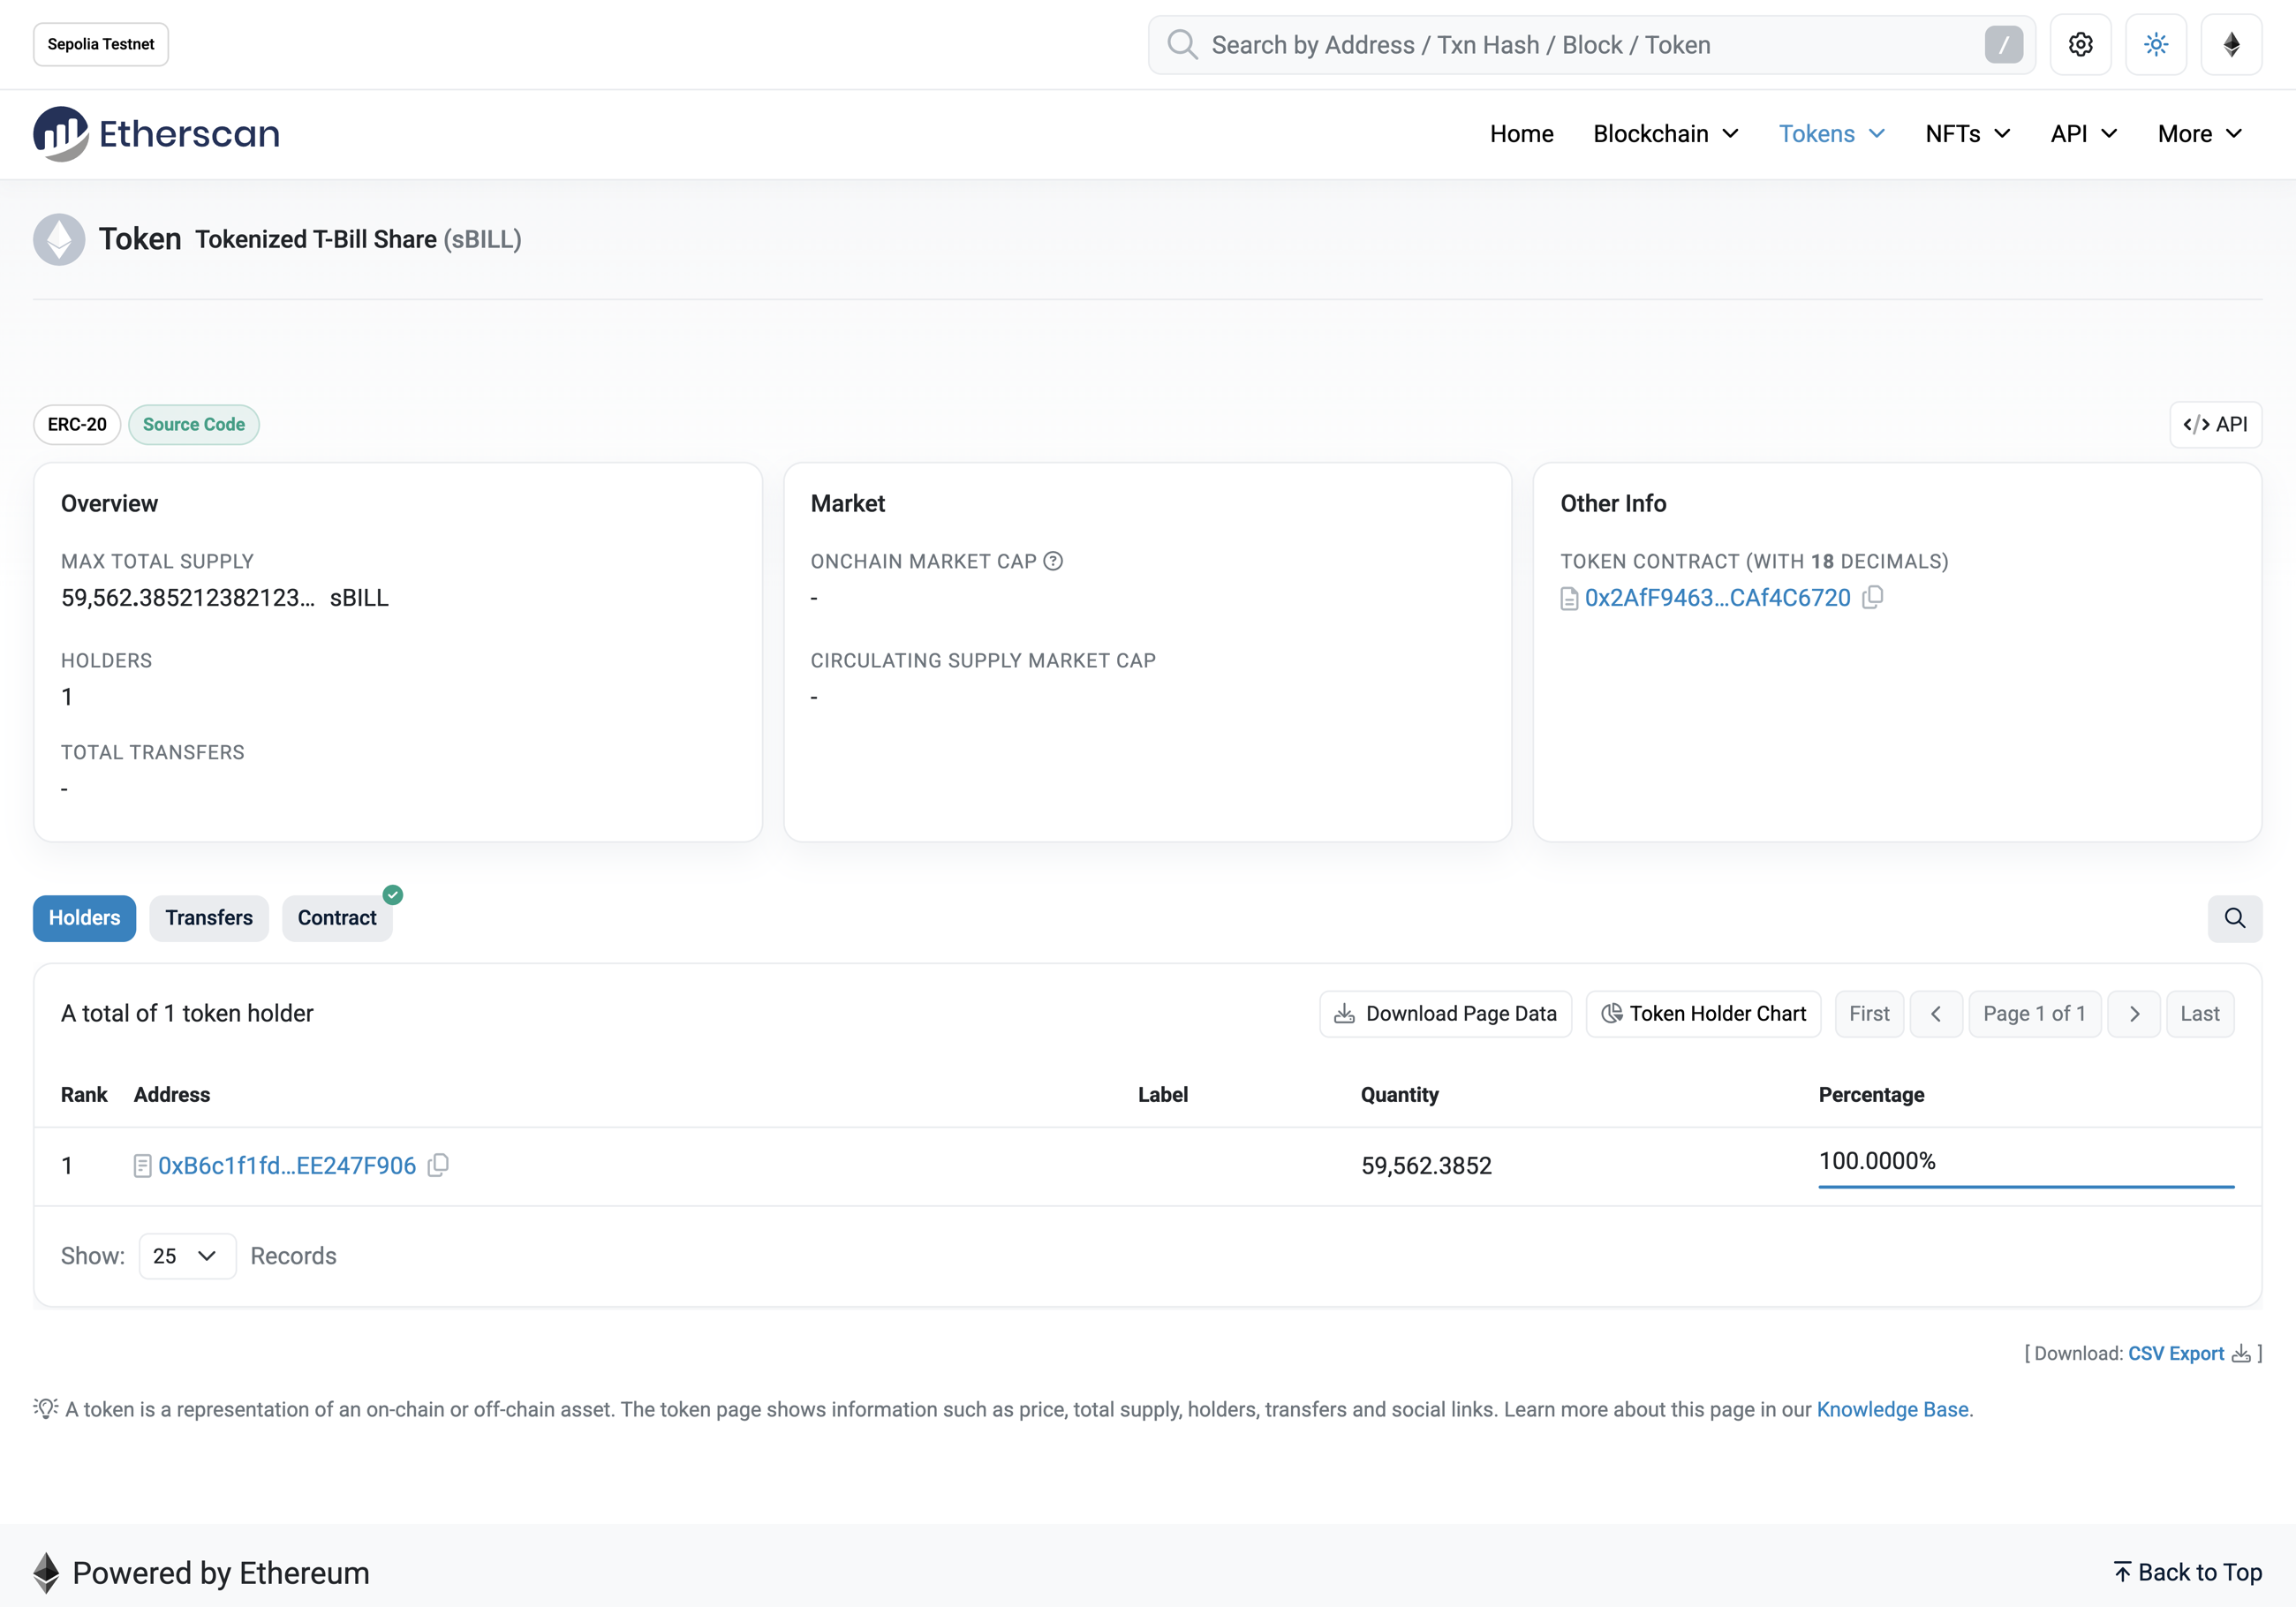
\includegraphics[width=\textwidth]{figures/screens/es_token.png}
\caption{\textbf{Our minted token on Sepolia.} \texttt{Tokenized T-Bill Share (sBILL)}, ERC-20, 18
decimals, with the green \emph{Source Code} badge. The supply shown is the sBILL the demo funds
subscribed for.}
\end{figure}

\begin{figure}[h!]\centering
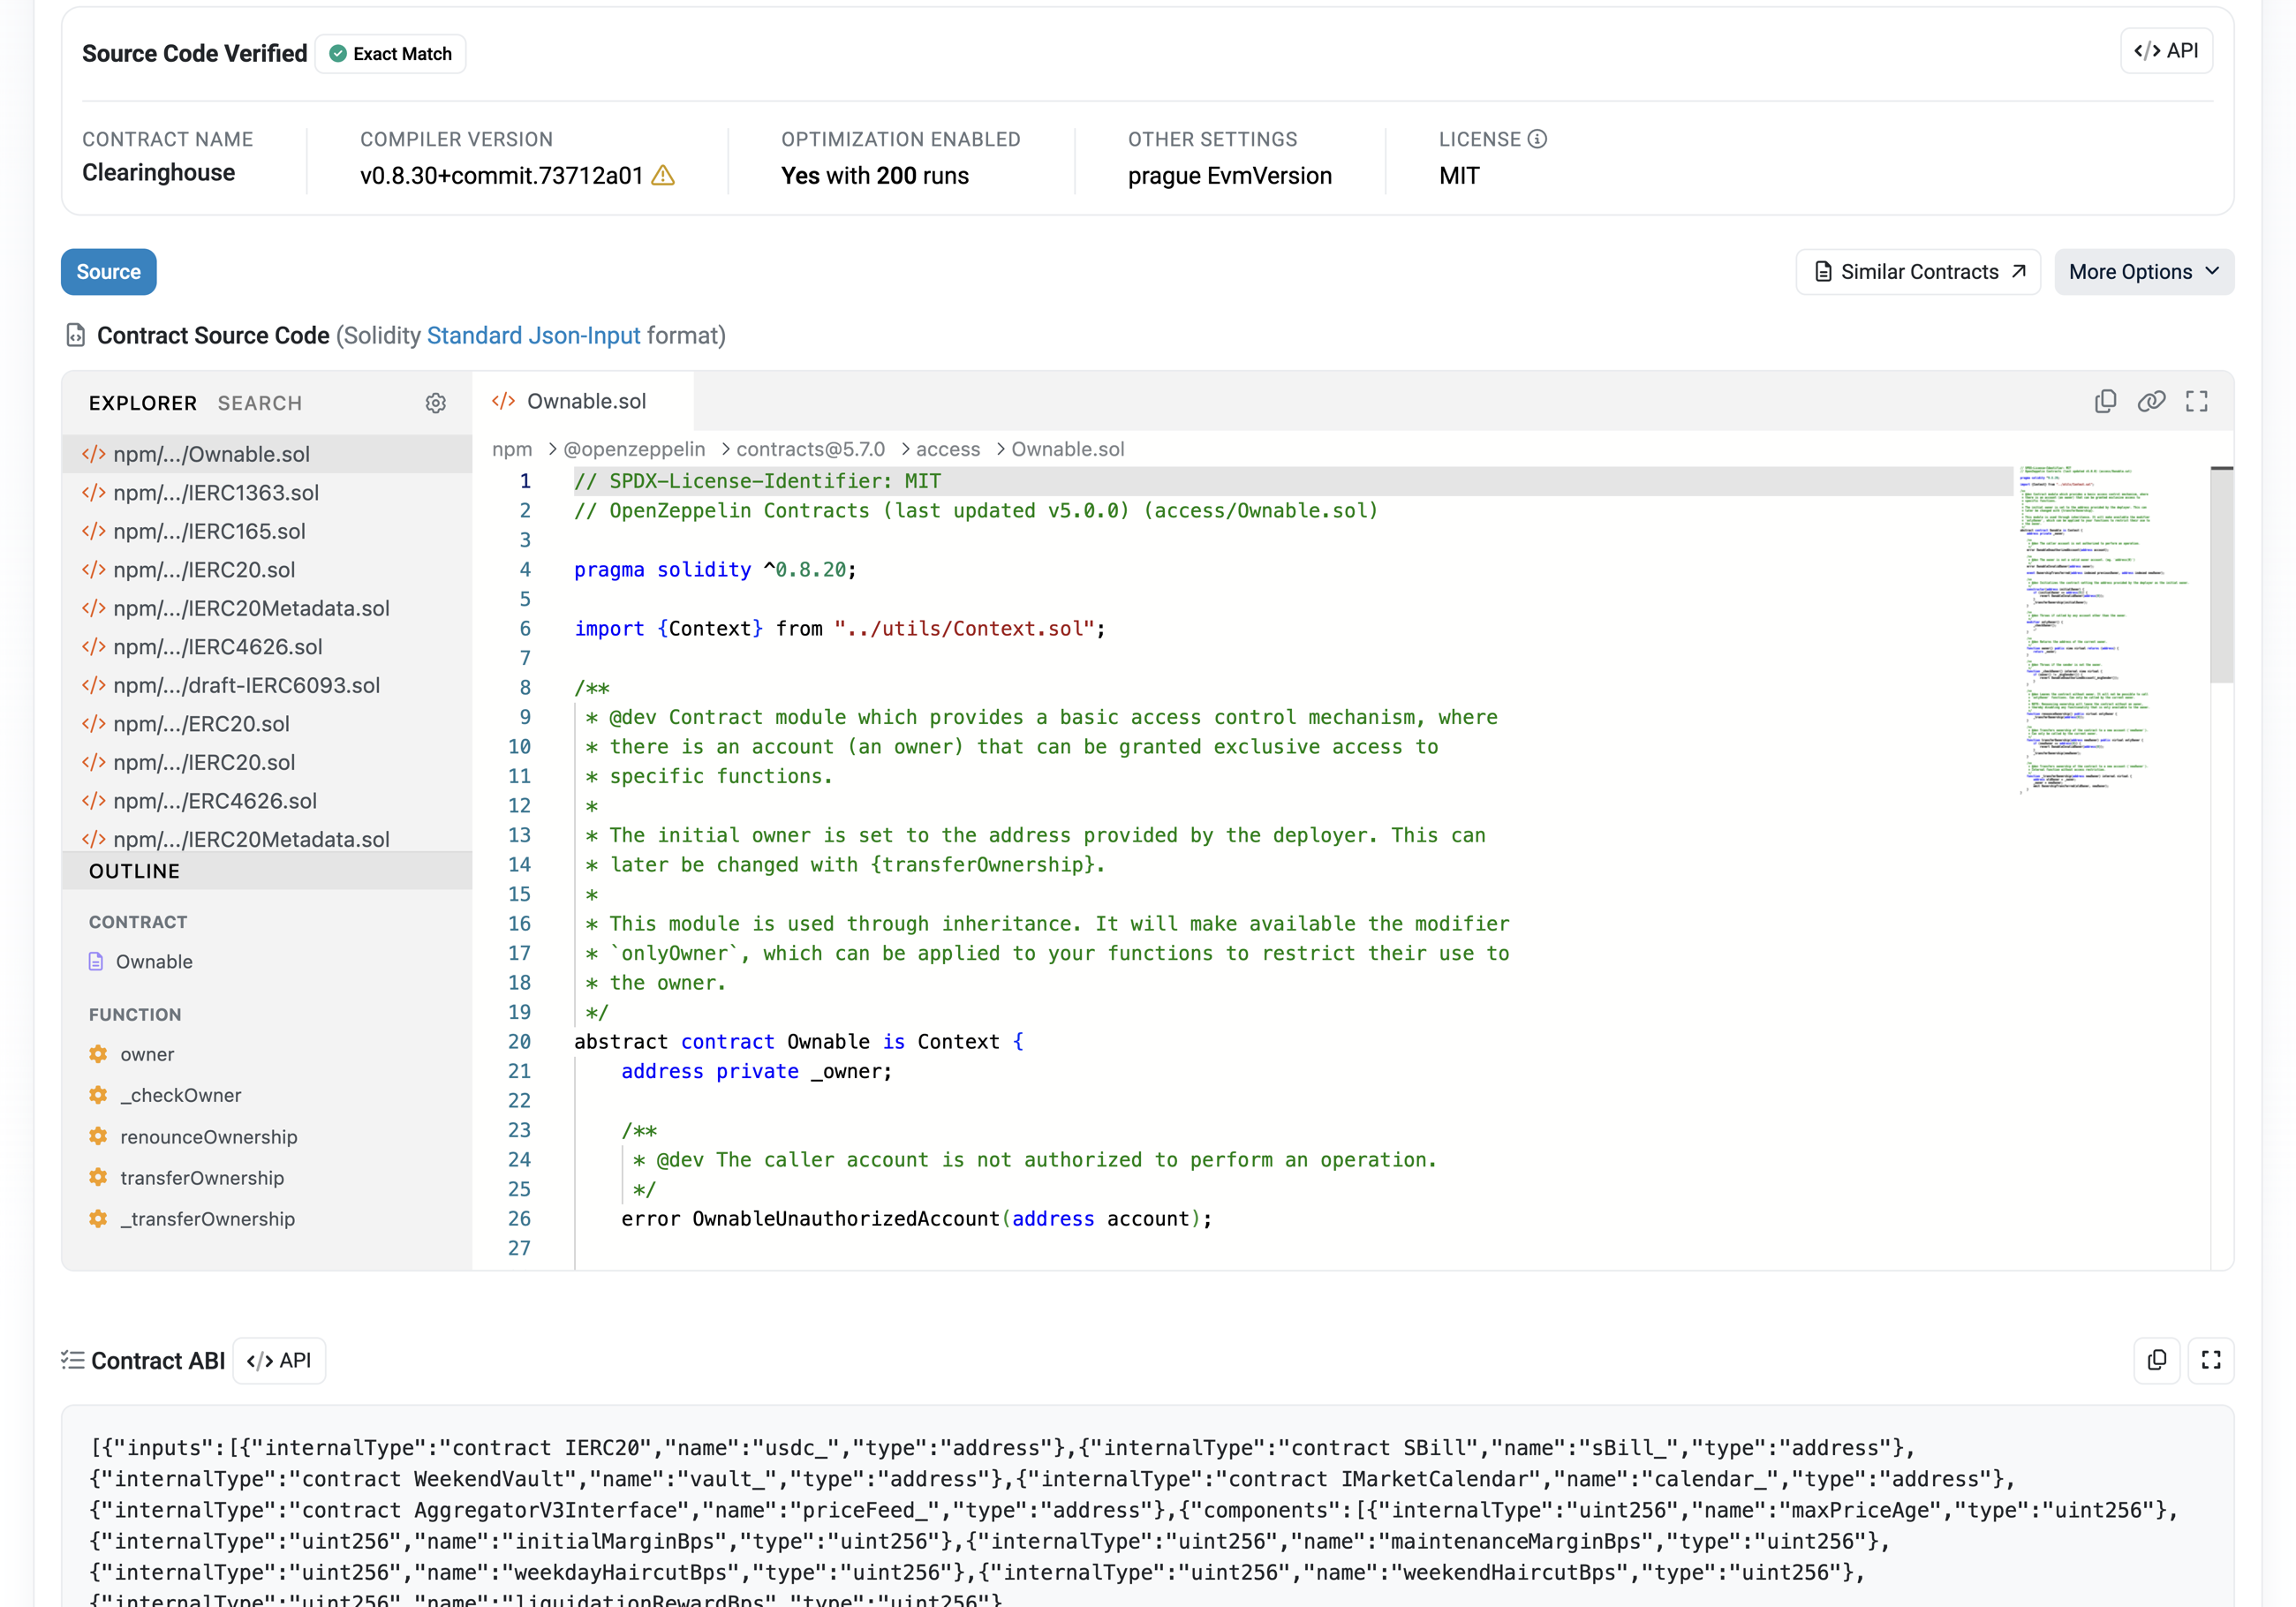
\includegraphics[width=\textwidth]{figures/screens/es_verified.png}
\caption{\textbf{Verified source, and the compiler settings behind it.} \texttt{Clearinghouse} on
Etherscan: \emph{Source Code Verified --- Exact Match}, \texttt{v0.8.30+commit.73712a01}, optimizer
on at 200 runs, \texttt{prague} EVM version, MIT. These are exactly the settings tabulated in
\S\ref{sec:metadata}, read off the chain rather than off our own build. All sixteen contracts show
this badge.}
\end{figure}

\begin{figure}[h!]\centering
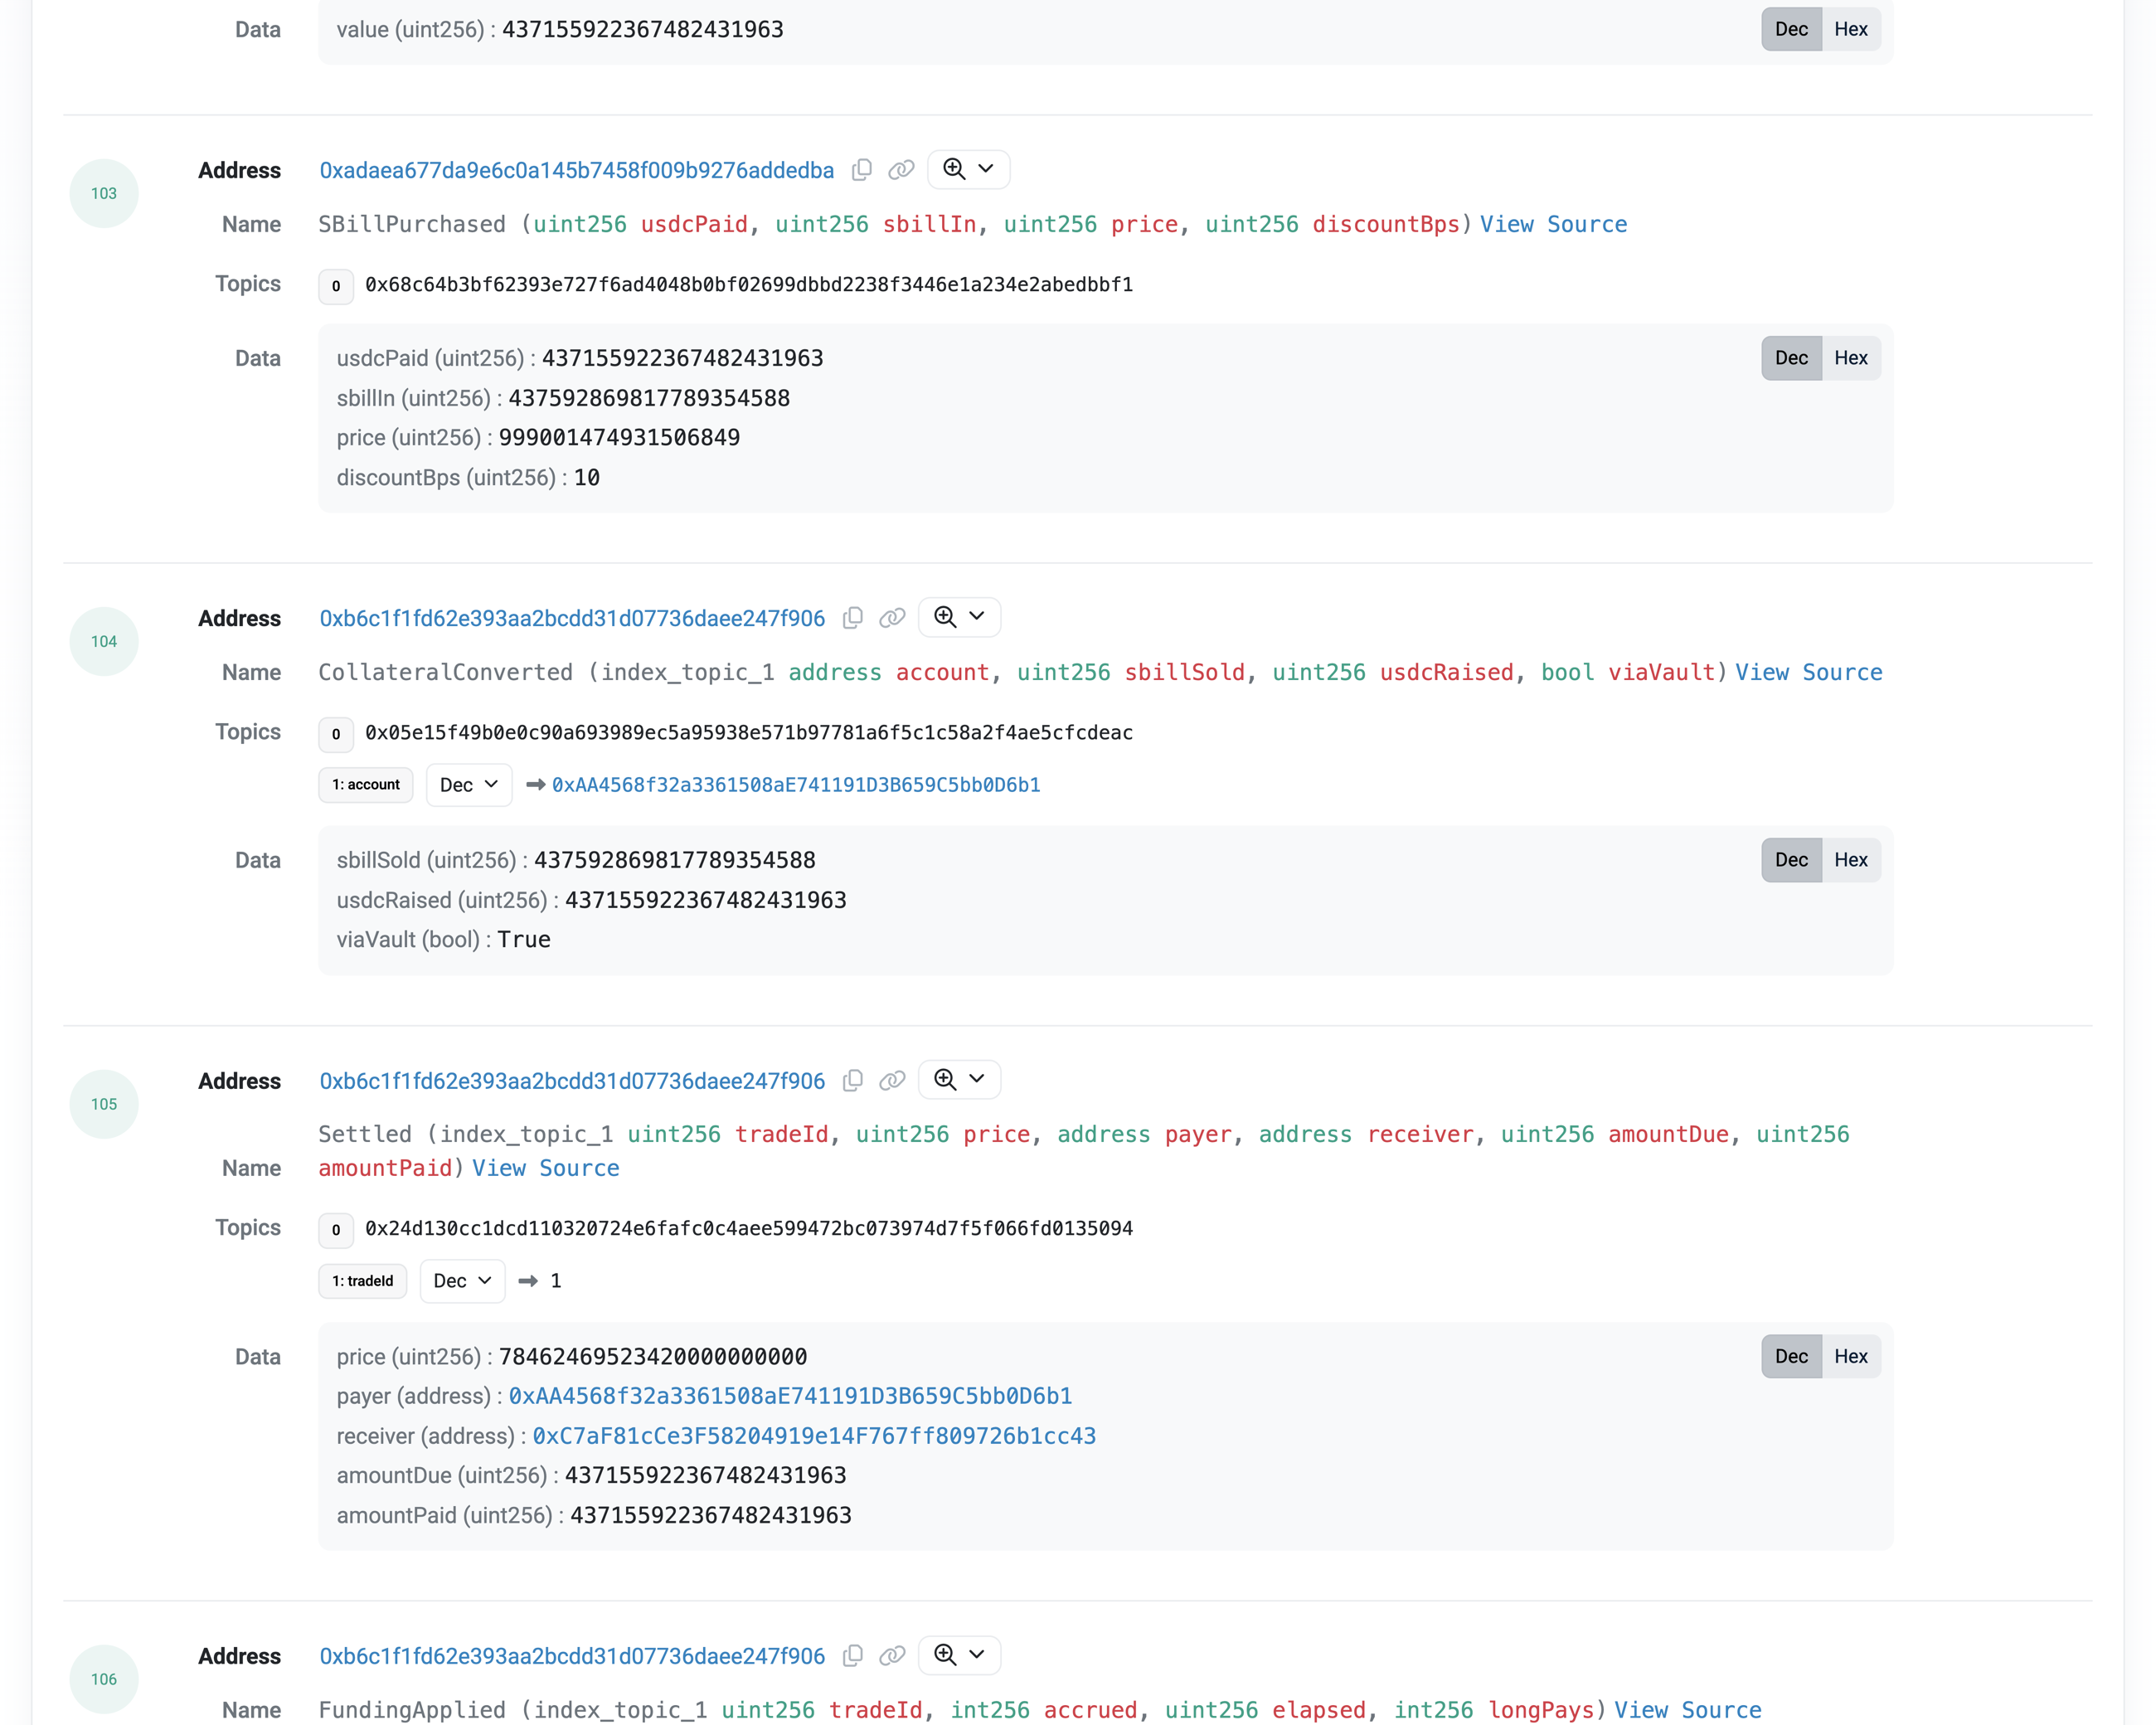
\includegraphics[width=\textwidth]{figures/screens/es_settlement.png}
\caption{\textbf{The weekend settlement, event by event --- this is the project's central claim.}
The sBILL \texttt{Transfer} moves 437.592869817789354588 from the clearinghouse to the vault; the
tUSDC \texttt{Transfer} moves 437.155922367482431963 back; and \texttt{SBillPurchased} records
\texttt{price = 999001474931506849} and \texttt{discountBps = 10}. The loser held no cash, the
T-bill market was shut, and the winner was paid anyway. Every one of those figures appears in the
reconciliation table of Appendix~\ref{app:recon}, matched to the wei.}
\end{figure}

\begin{figure}[h!]\centering
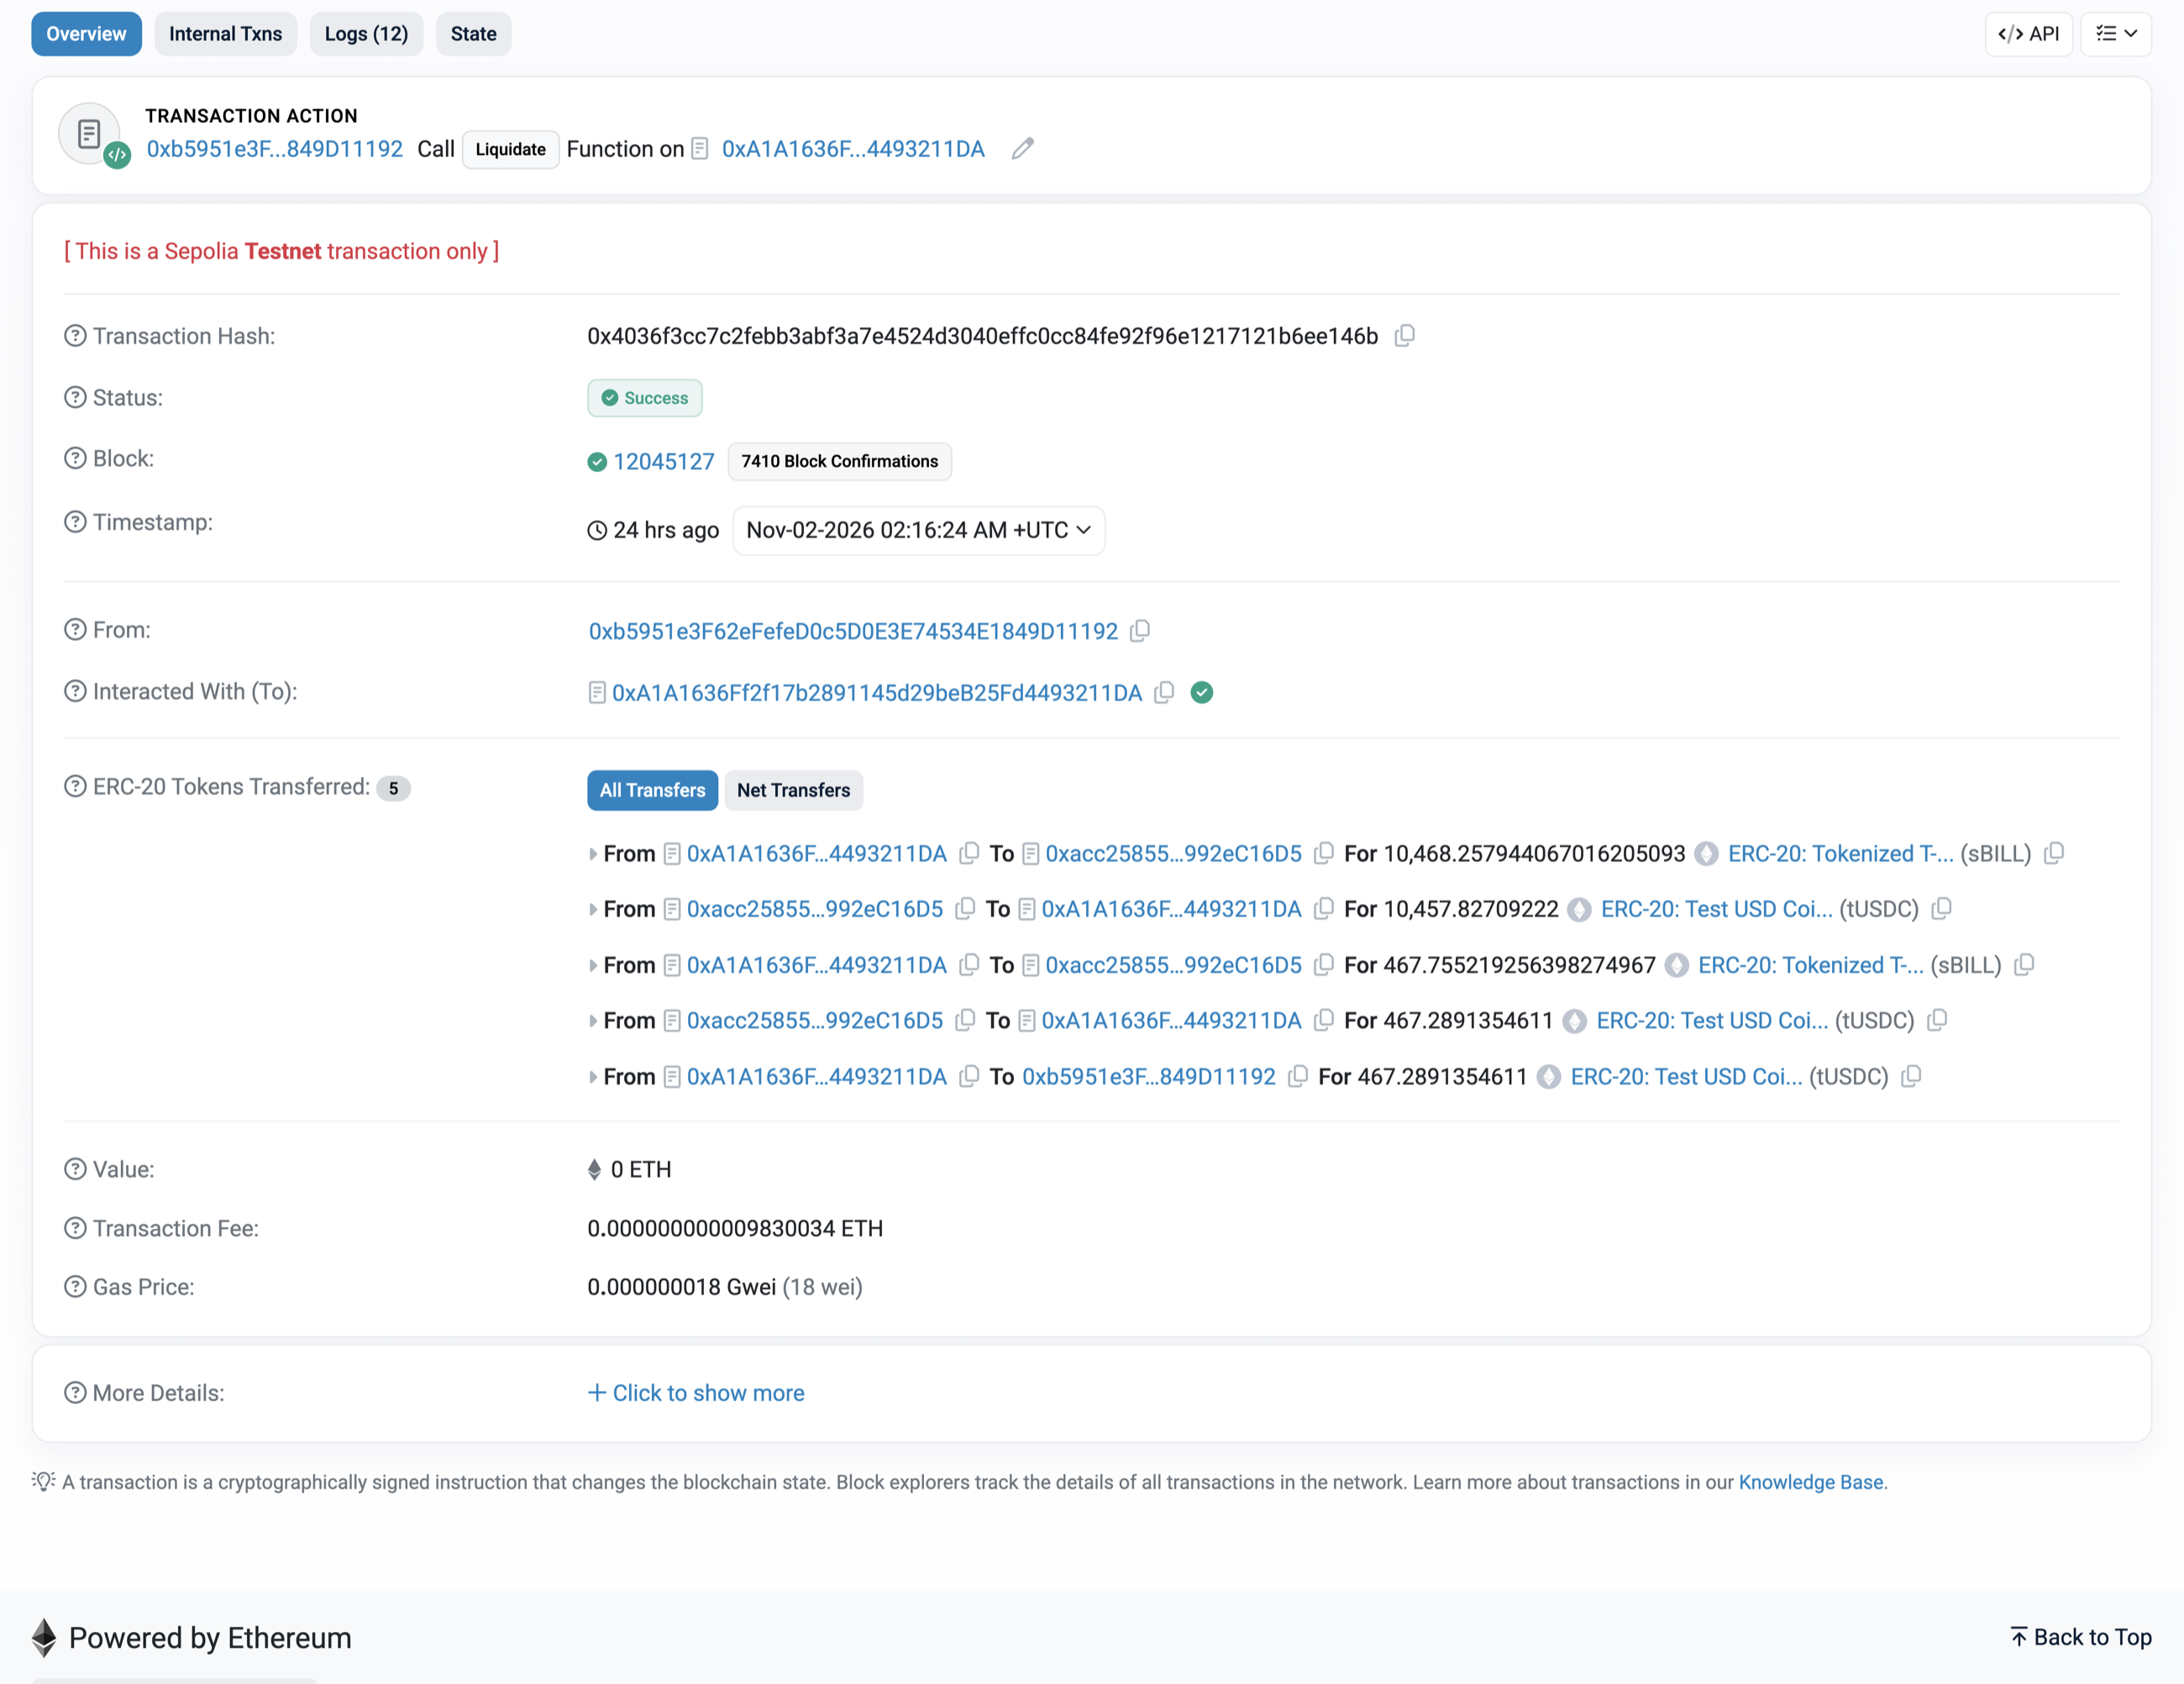
\includegraphics[width=\textwidth]{figures/screens/es_liquidation.png}
\caption{\textbf{A real liquidation, on the clearly labelled stress set.} A \texttt{Liquidate} call
that succeeded, with five ERC-20 transfers: the losing side's sBILL sold to the vault, cash returned,
and \textbf{467.2891354611 tUSDC paid to the liquidator} --- the 0.5\% reward, and the same
\$467.29 the model predicted in \S\ref{sec:liverun}. \textbf{This set's Bitcoin price is a mock;}
the Main set uses the real Chainlink feed.}
\end{figure}

\clearpage

\subsection{The settings the contracts actually run with}\label{sec:oracle}

These come from \texttt{config/protocol.json} at deployment. \textbf{If any document disagrees with a
contract, the contract wins} — and \S\ref{sec:reconcile} reads each of these back off the chain to
prove no document does.

\begin{center}
\small
\begin{tabular}{@{}p{5.2cm}p{2.4cm}p{7.6cm}@{}}
\toprule
\textbf{Setting} & \textbf{Value} & \textbf{Where it binds} \\
\midrule
Initial margin & 20\% & Caps opening leverage at $5\times$ \\
Maintenance margin & 10\% & The liquidation trigger \\
sBILL haircut, market open & 1\% & sBILL counts at 99\% of NAV \\
sBILL haircut, market closed & 3\% & sBILL counts at 97\% of NAV \\
sBILL interest & 4.00\% simple & Accrues on the clock, weekends included \\
Vault discount & 10bp & Owner-adjustable up to a 1\% hard cap, only while the market is open \\
Liquidation reward & 0.5\% of notional & Paid to whoever calls \texttt{liquidate} \\
Funding cap & 0.1\% per hour & The largest rate the owner can post \\
Oldest accepted price & 2 hours & Above the feed's roughly 1-hour heartbeat \\
\bottomrule
\end{tabular}
\end{center}

\subsection{The front end}\label{sec:frontend}

Seven pages, built on Scaffold-ETH 2 with Next.js, wagmi, viem and RainbowKit. It reads the live
Sepolia contracts with no wallet connected, and a dropdown switches between the Main, Demo and
Stress sets. Every screenshot below was taken from the running application reading Sepolia.

\begin{figure}[h!]\centering
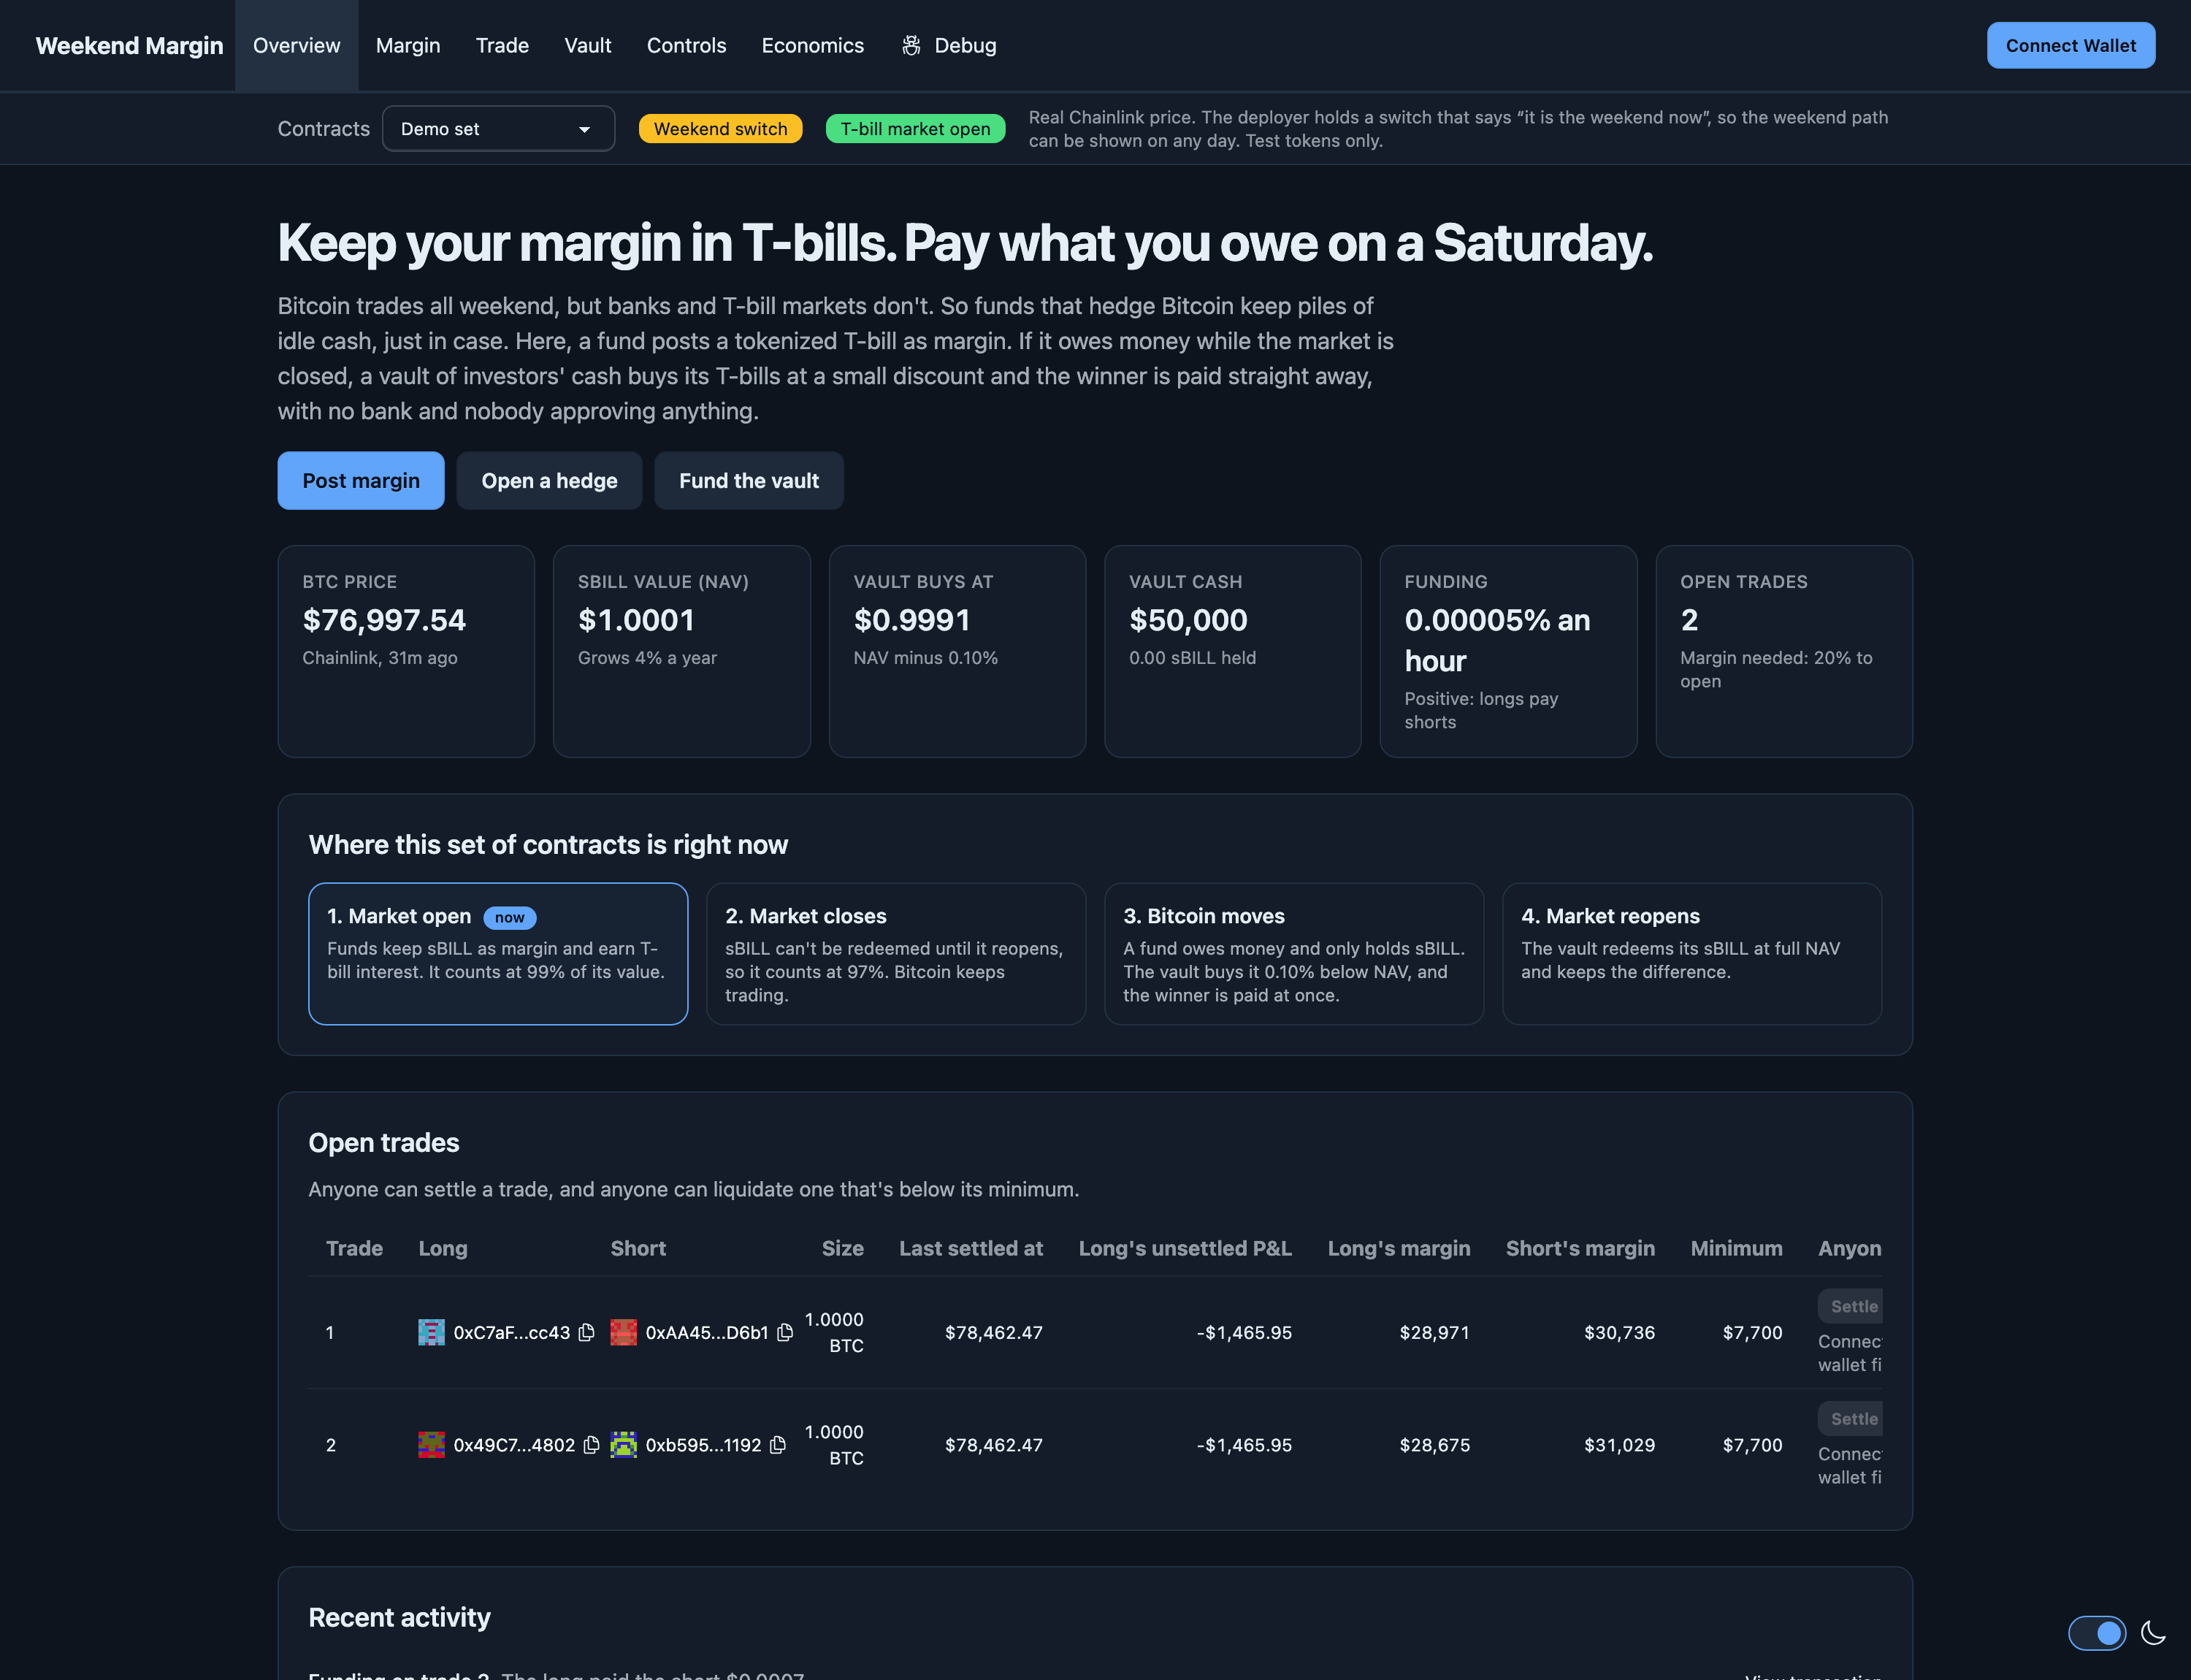
\includegraphics[width=\textwidth]{figures/screens/app_home.png}
\caption{Overview. The live Chainlink price, the sBILL NAV, the vault's cash, the funding rate and
the open trades, all read from the deployed contracts. The yellow badge says that the deployer holds
the demo weekend switch.}
\end{figure}

\begin{figure}[h!]\centering
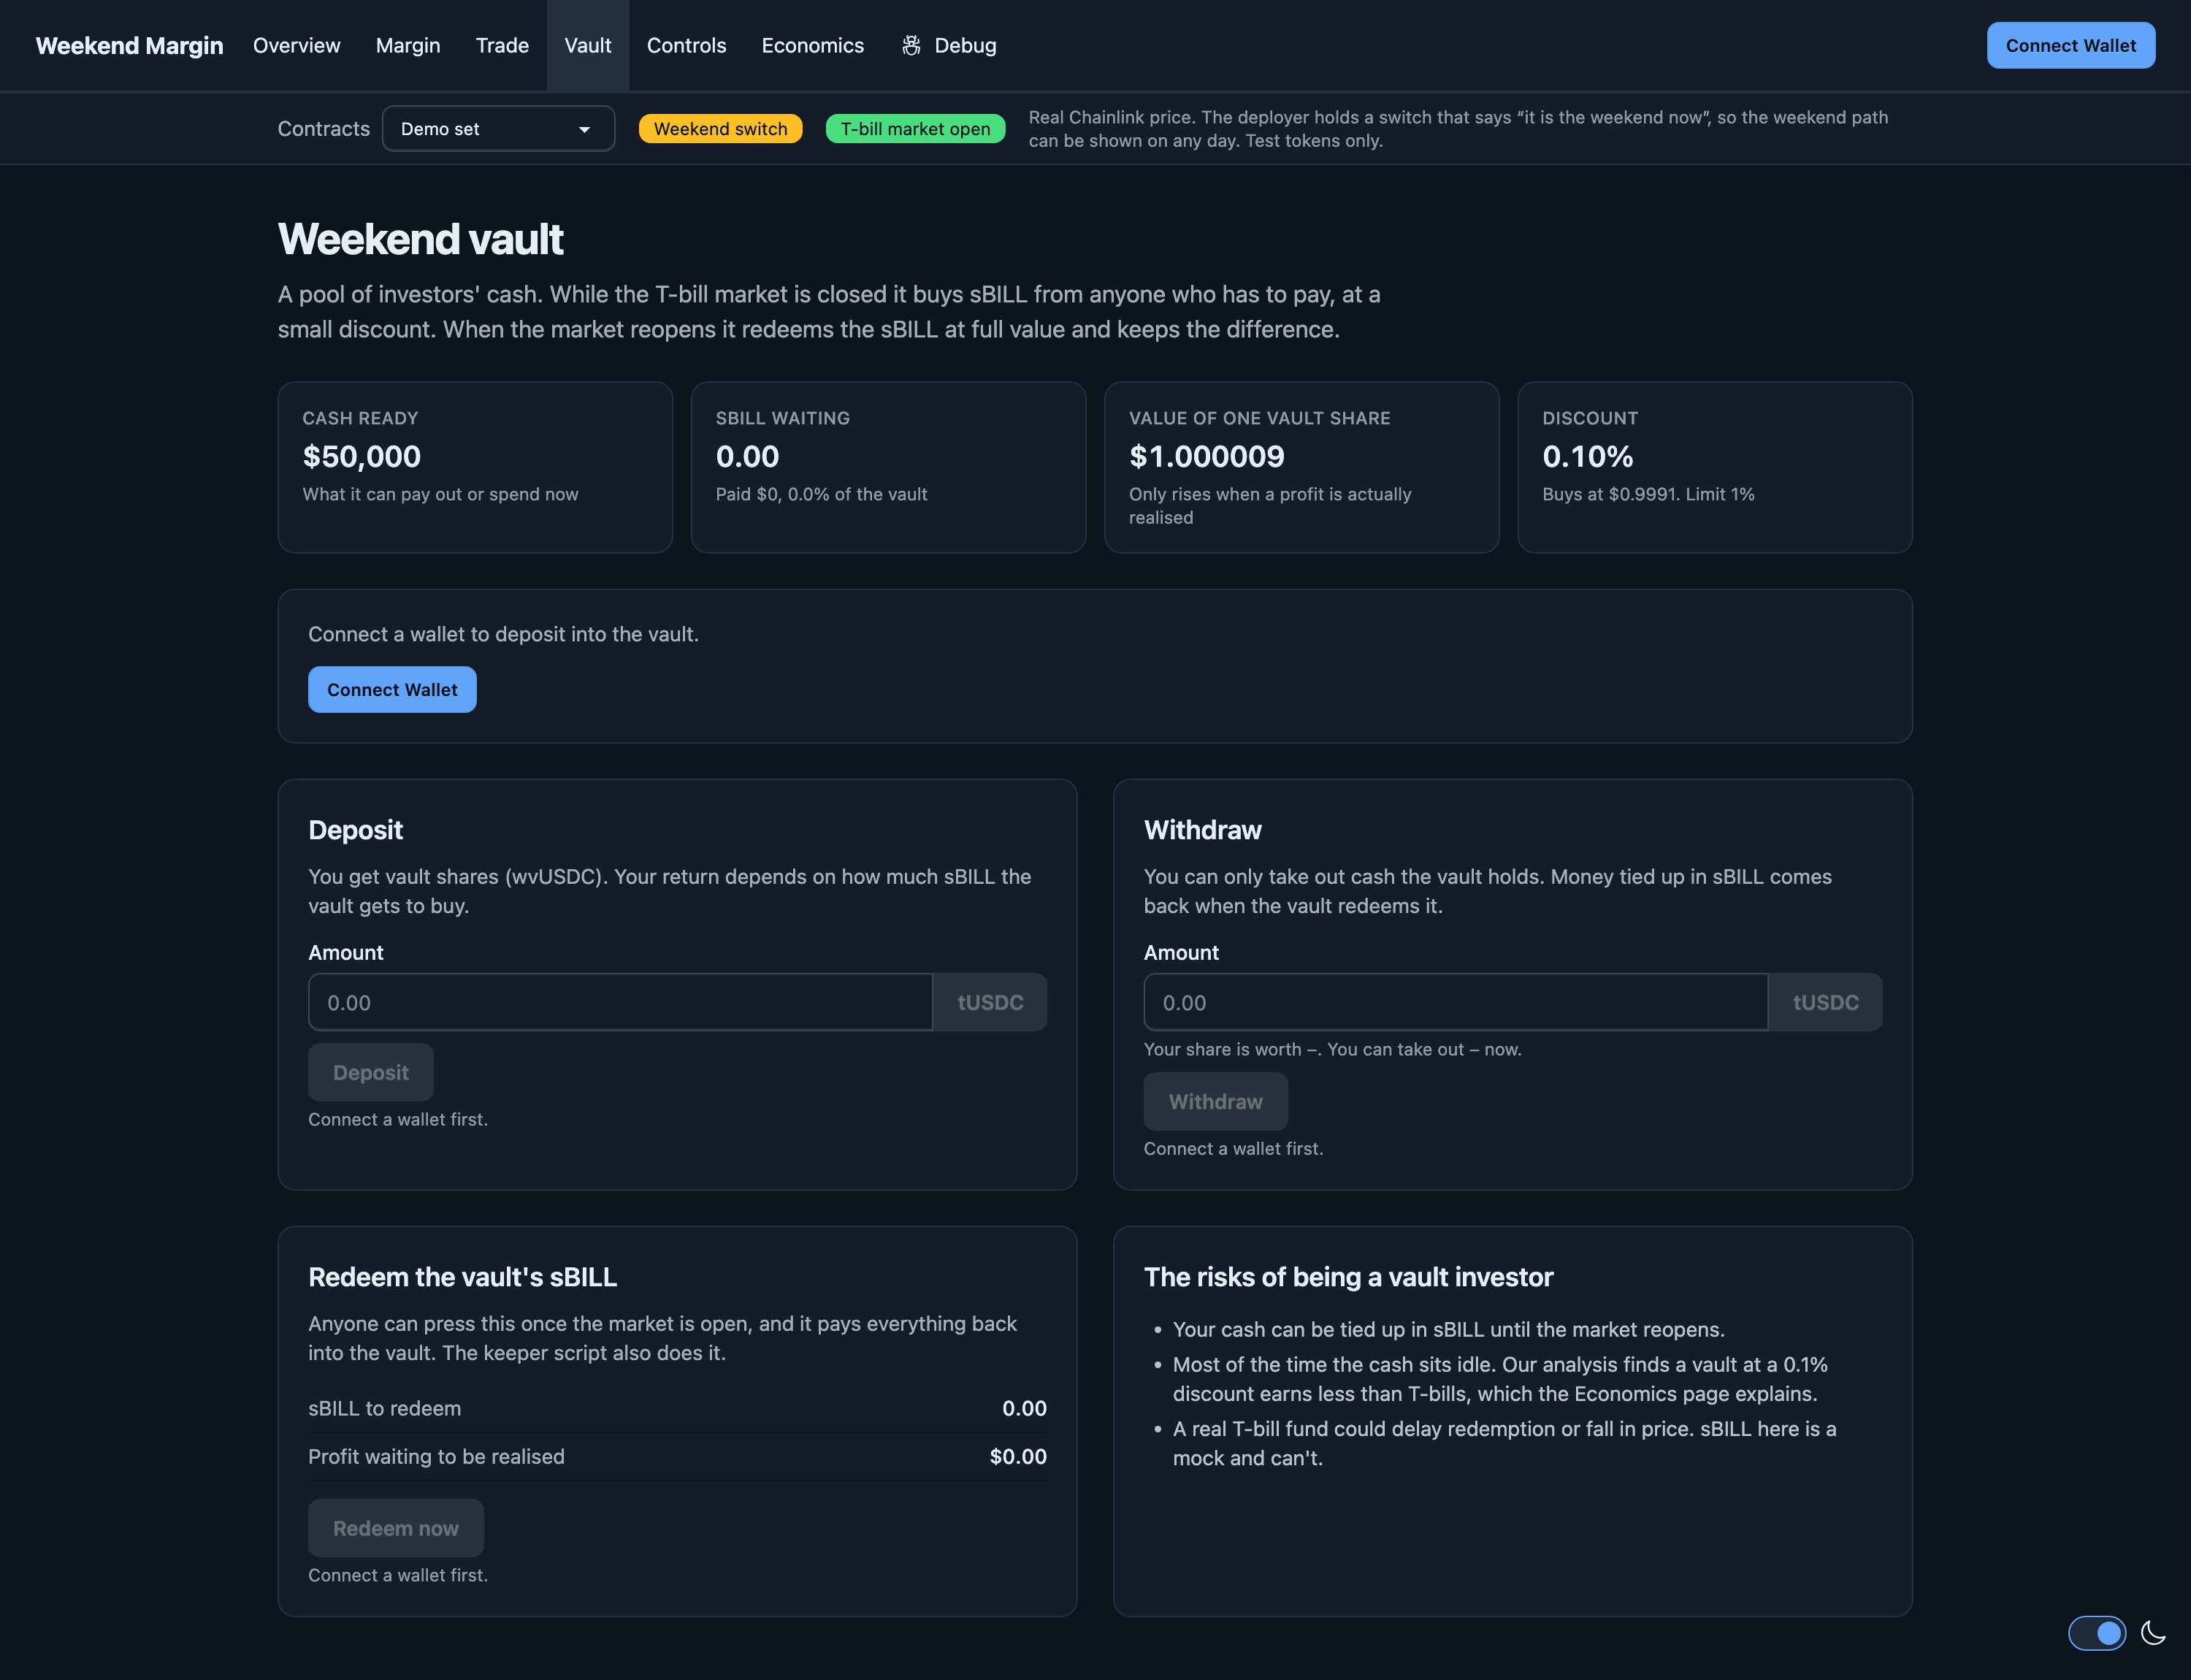
\includegraphics[width=\textwidth]{figures/screens/app_vault.png}
\caption{The vault. Cash ready, sBILL waiting for Monday, the share price — which only rises when a
profit is actually realised — and the discount with its hard limit. The risks of being a depositor
are stated on the page, not buried in a document.}
\end{figure}

\begin{figure}[h!]\centering
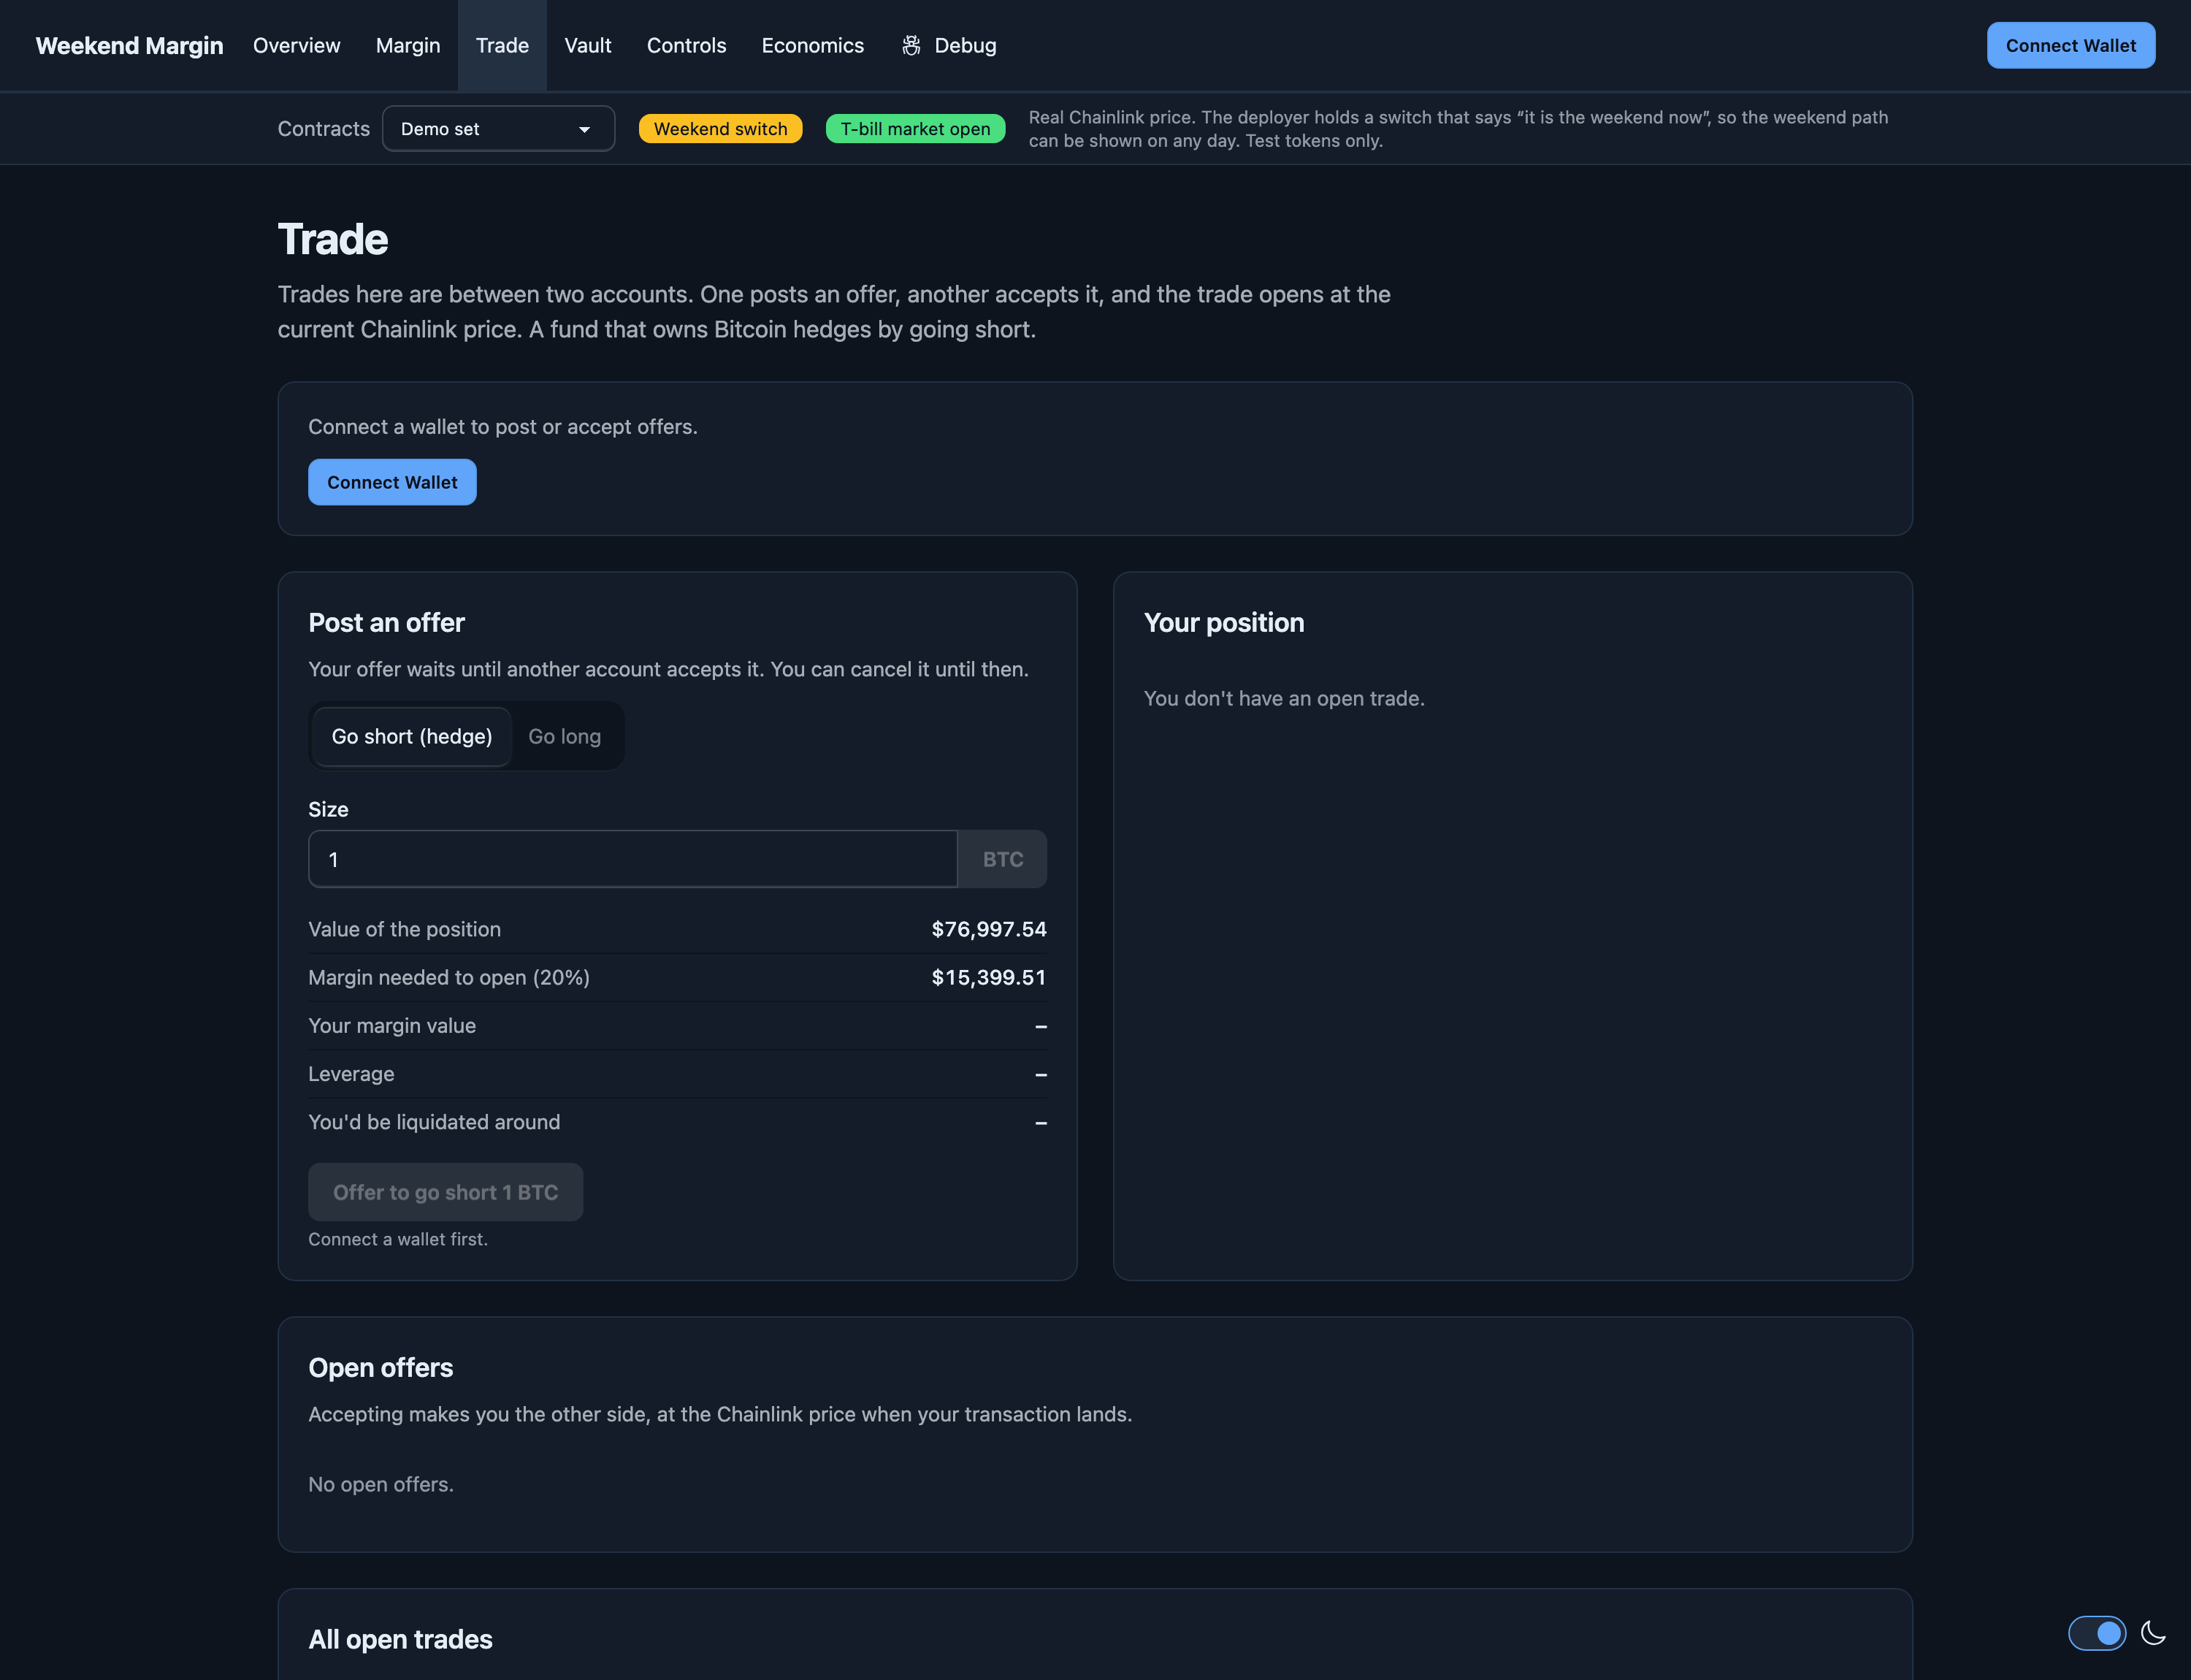
\includegraphics[width=\textwidth]{figures/screens/app_trade.png}
\caption{Trading. The liquidation price for \emph{both} sides is computed from the contract's own
formula as the inputs change, before anything is signed.}
\end{figure}

\begin{figure}[h!]\centering
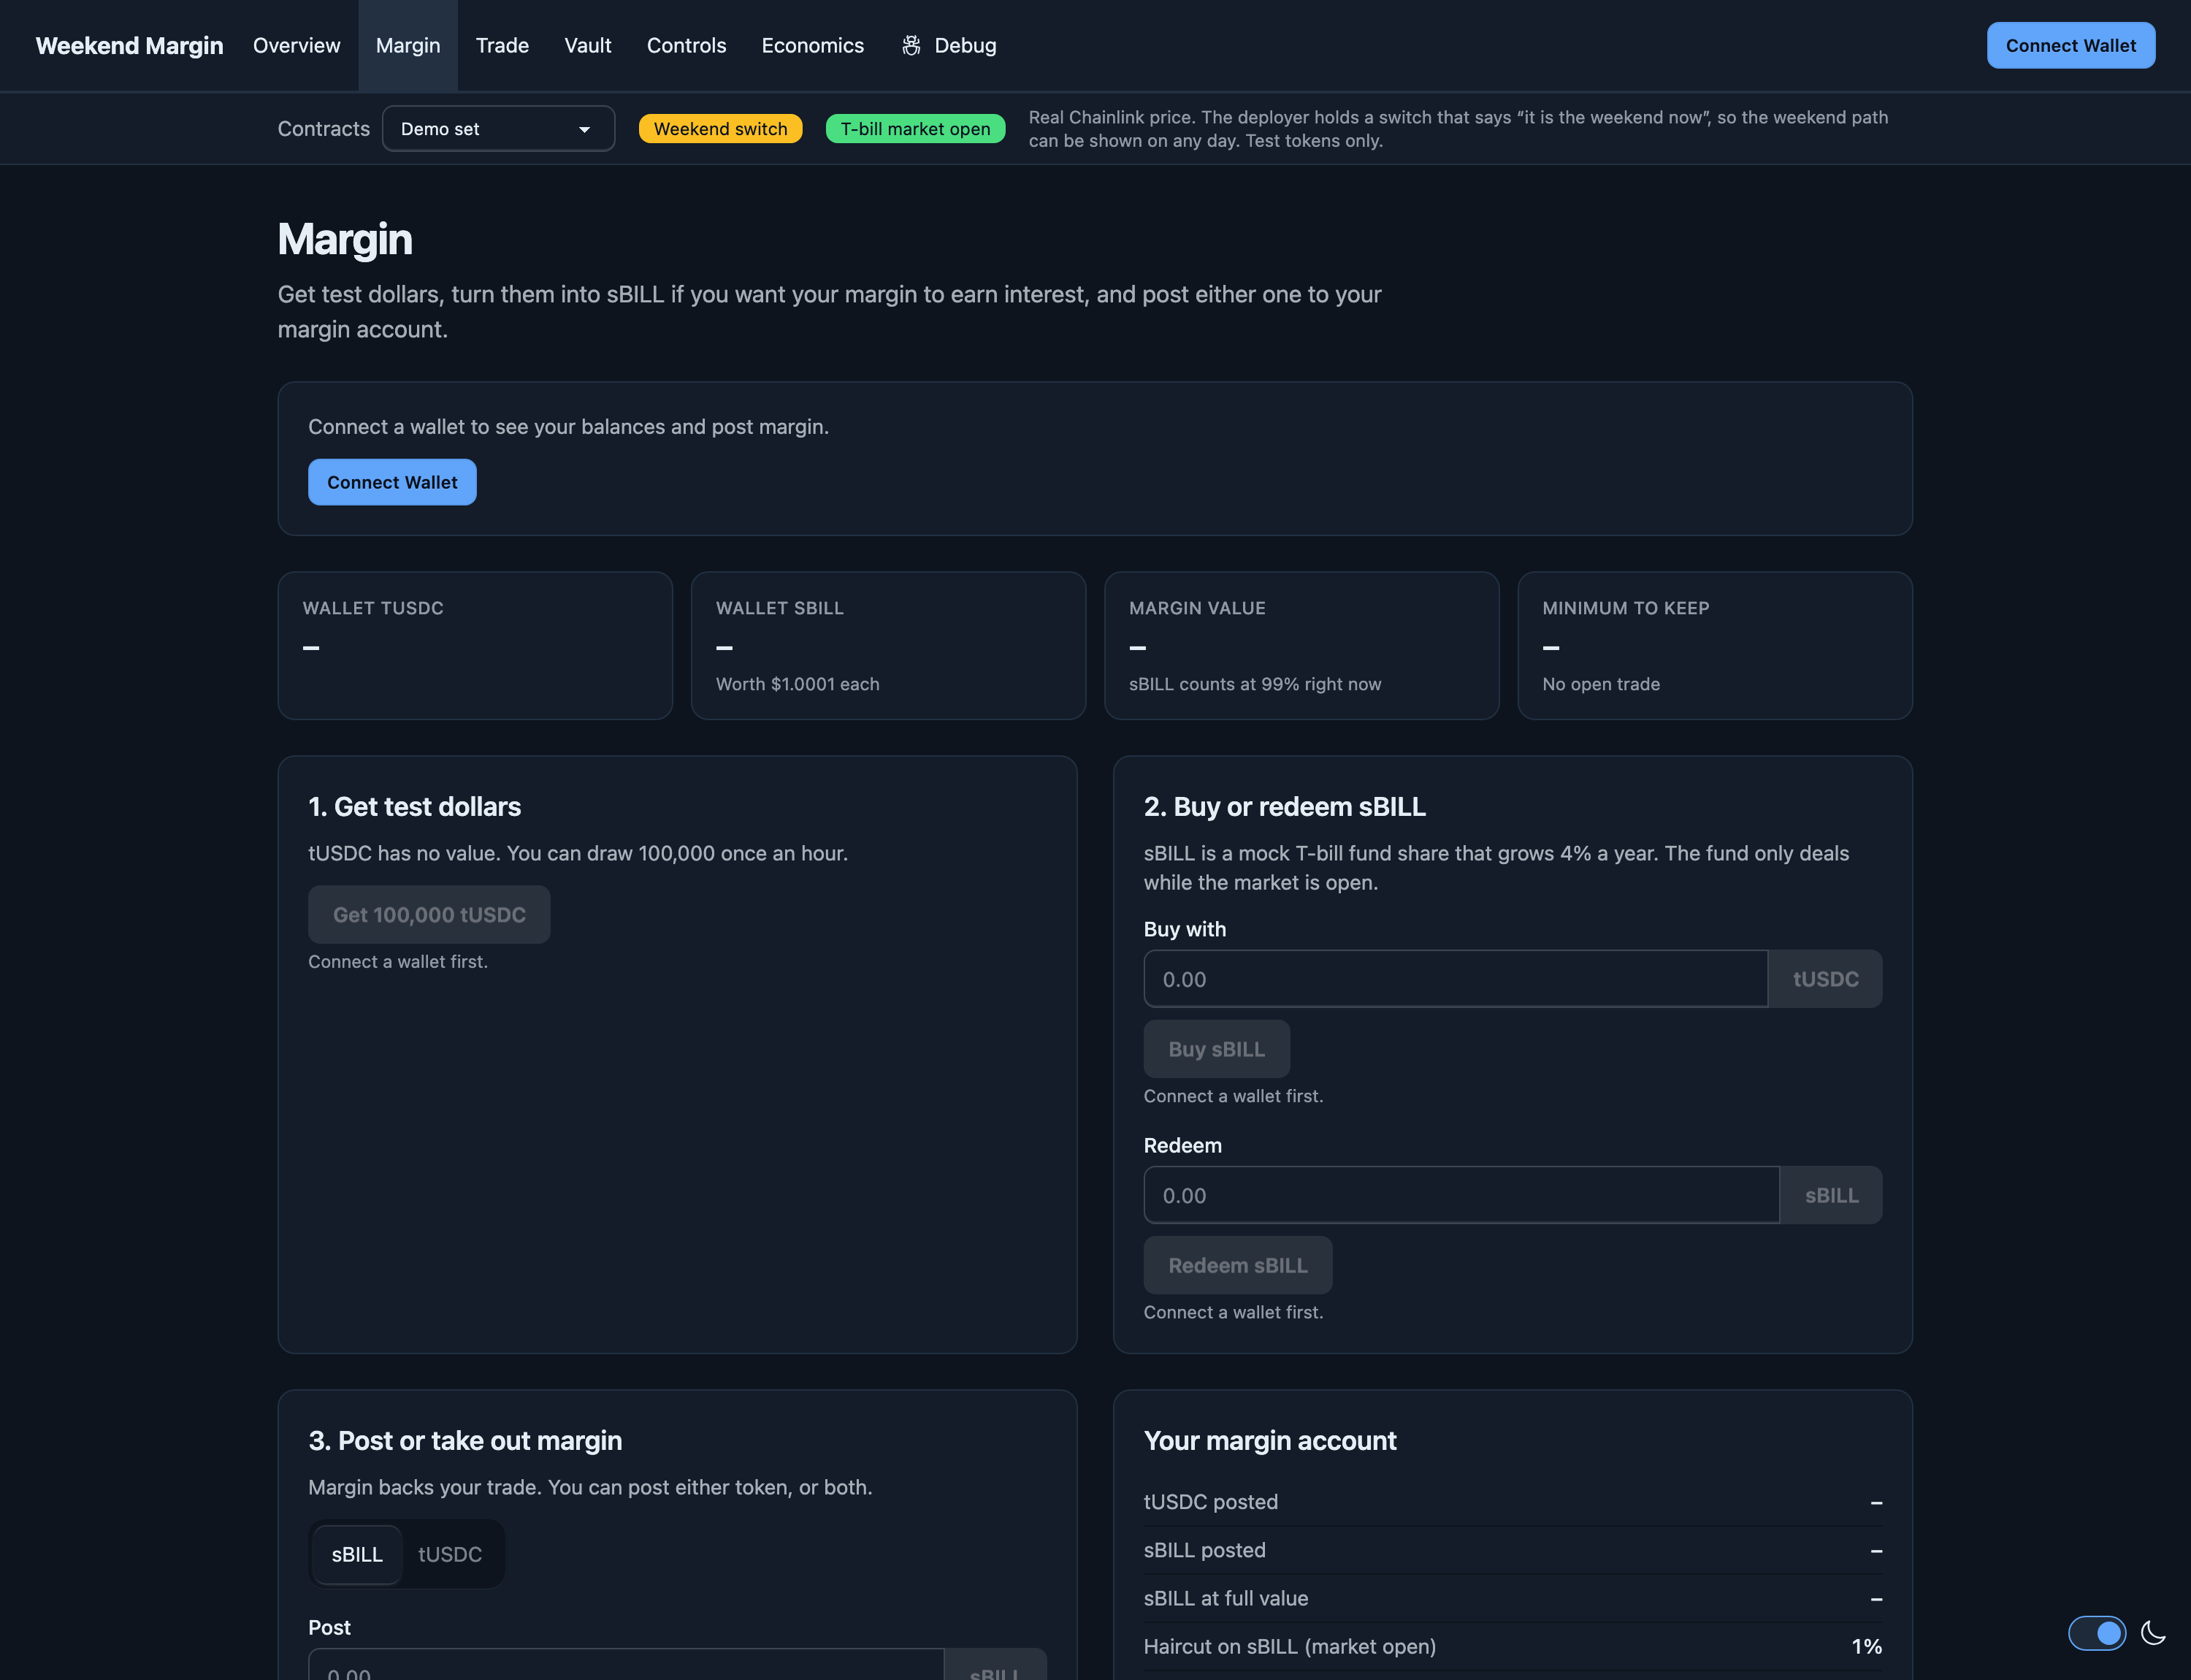
\includegraphics[width=\textwidth]{figures/screens/app_margin.png}
\caption{Margin. Deposits and withdrawals in tUSDC and sBILL, with the haircut applied live and
account health shown against both margin levels.}
\end{figure}

\begin{figure}[h!]\centering
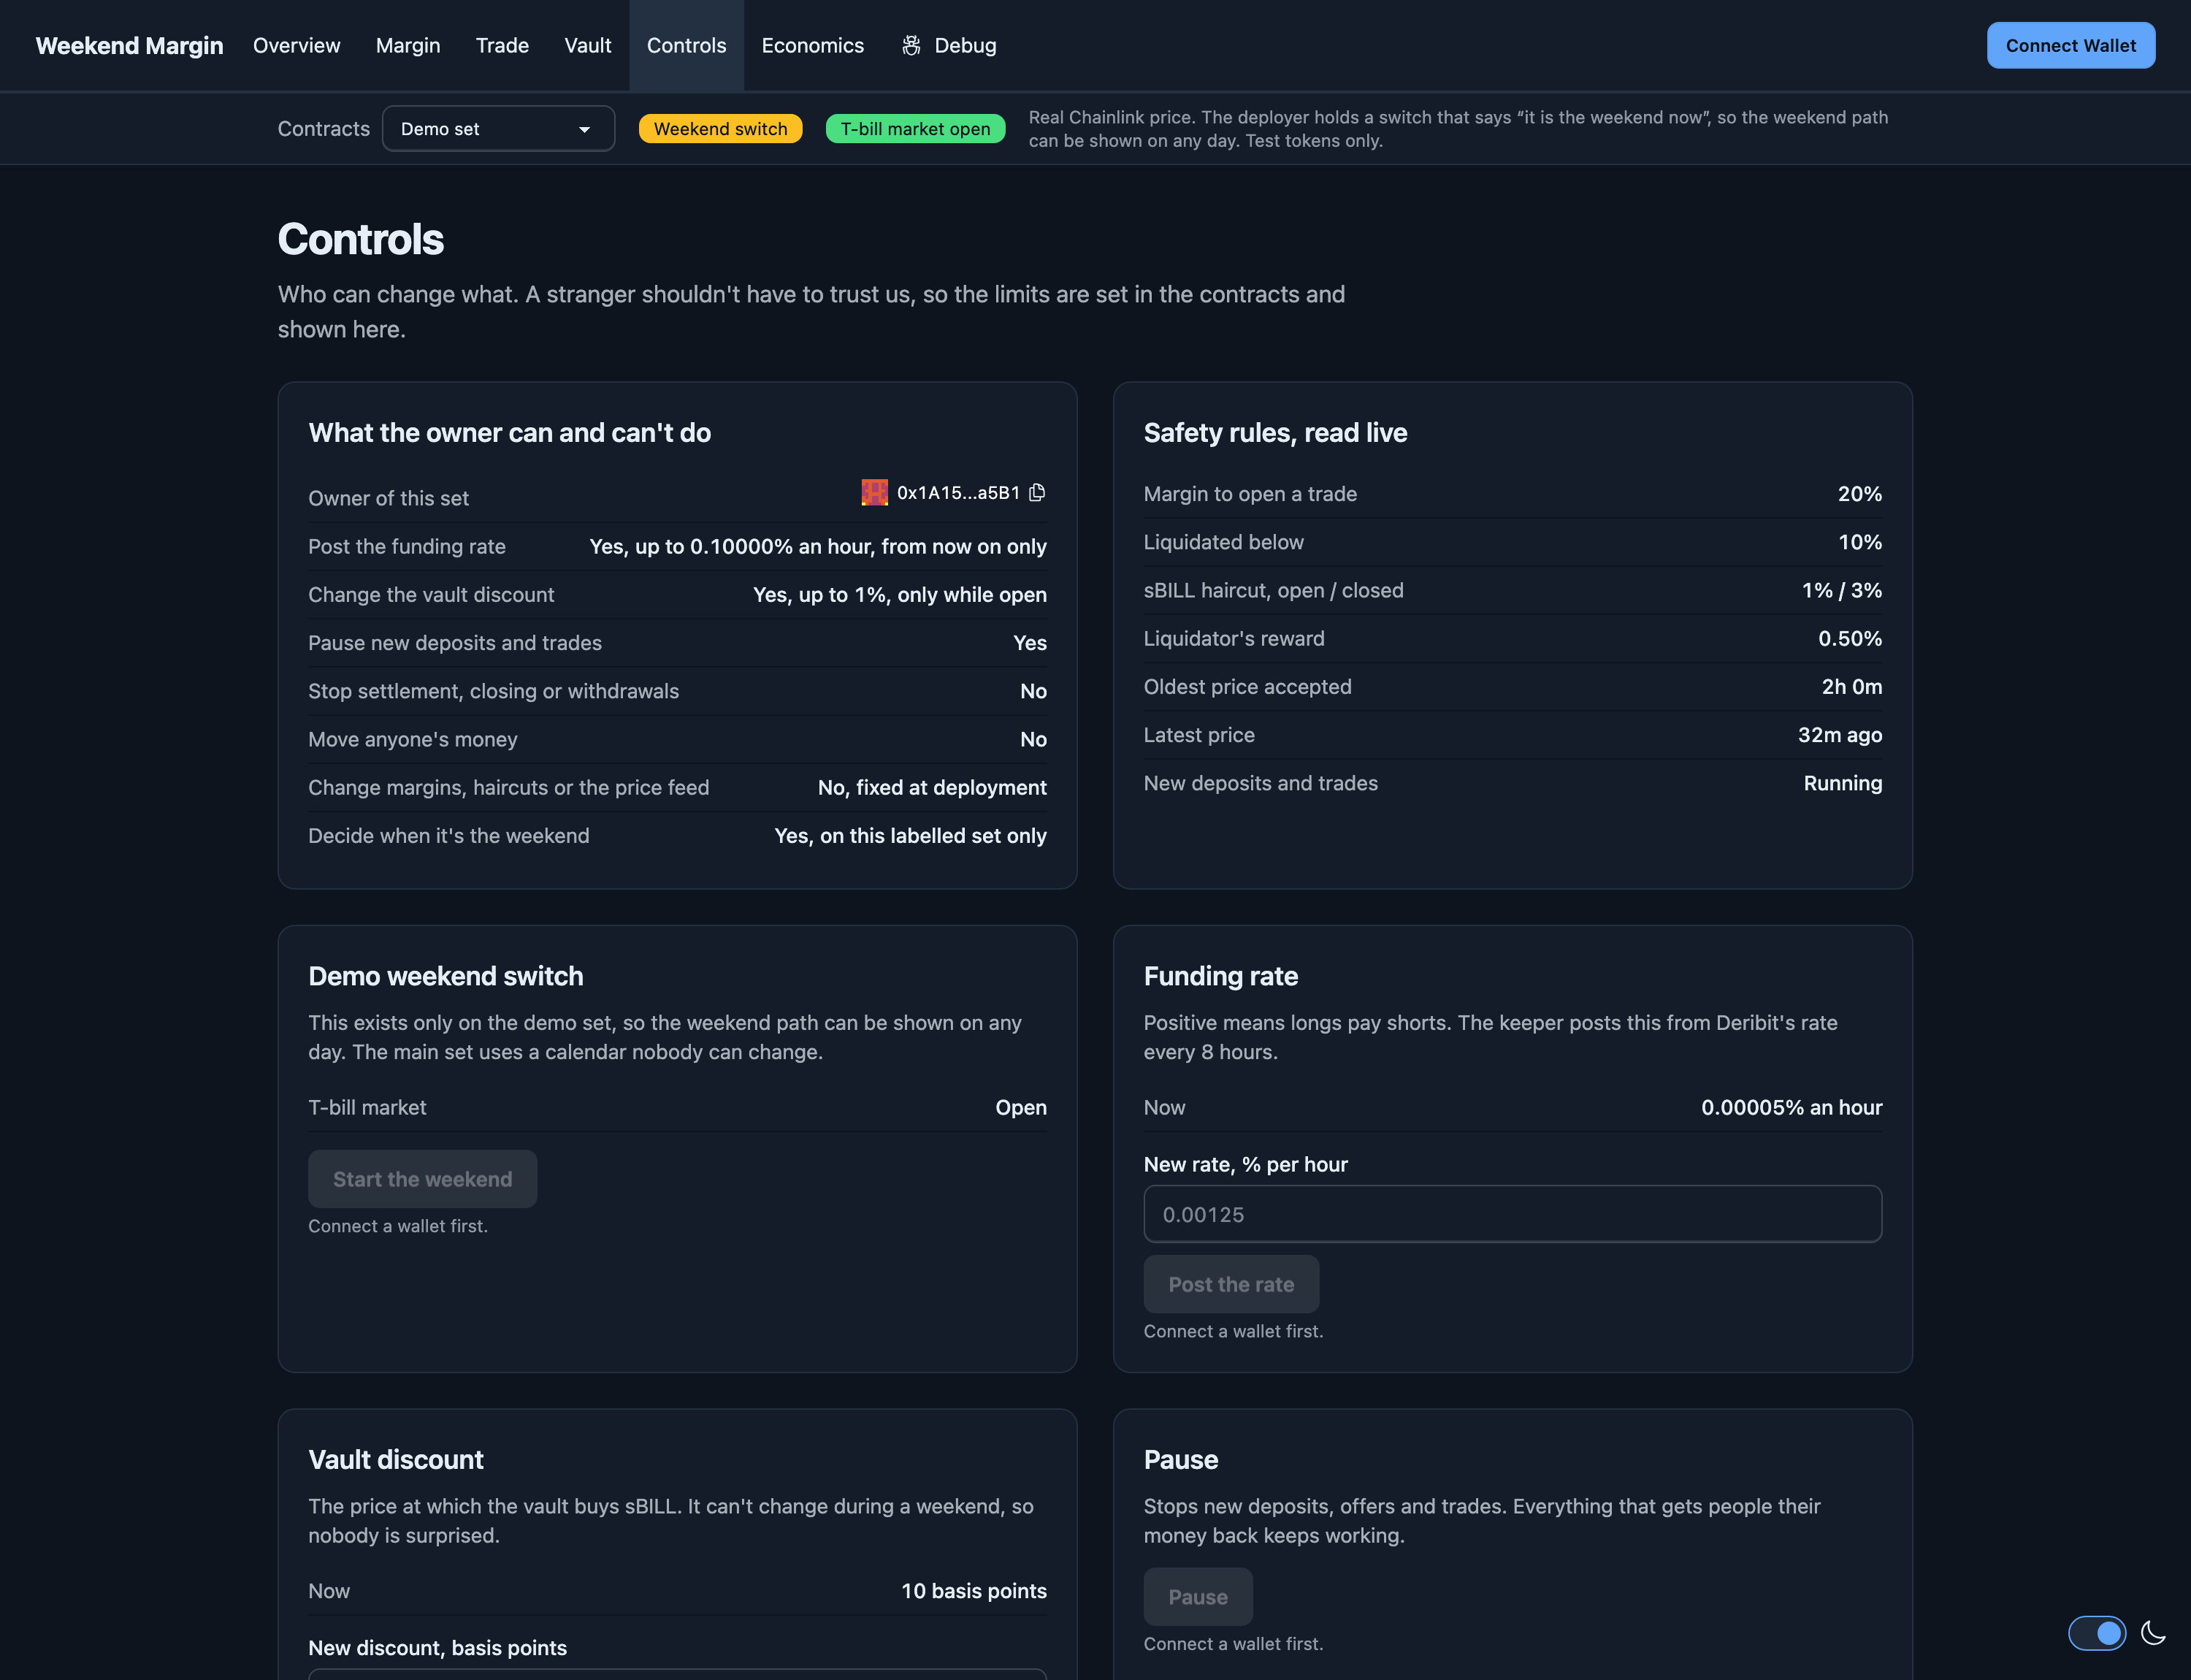
\includegraphics[width=\textwidth]{figures/screens/app_controls.png}
\caption{Controls. Every admin power, with its hard limit printed next to it. We put the owner's
powers on a page rather than in a footnote, because a stranger should be able to see exactly what we
can and cannot do to them.}
\end{figure}

\begin{figure}[h!]\centering
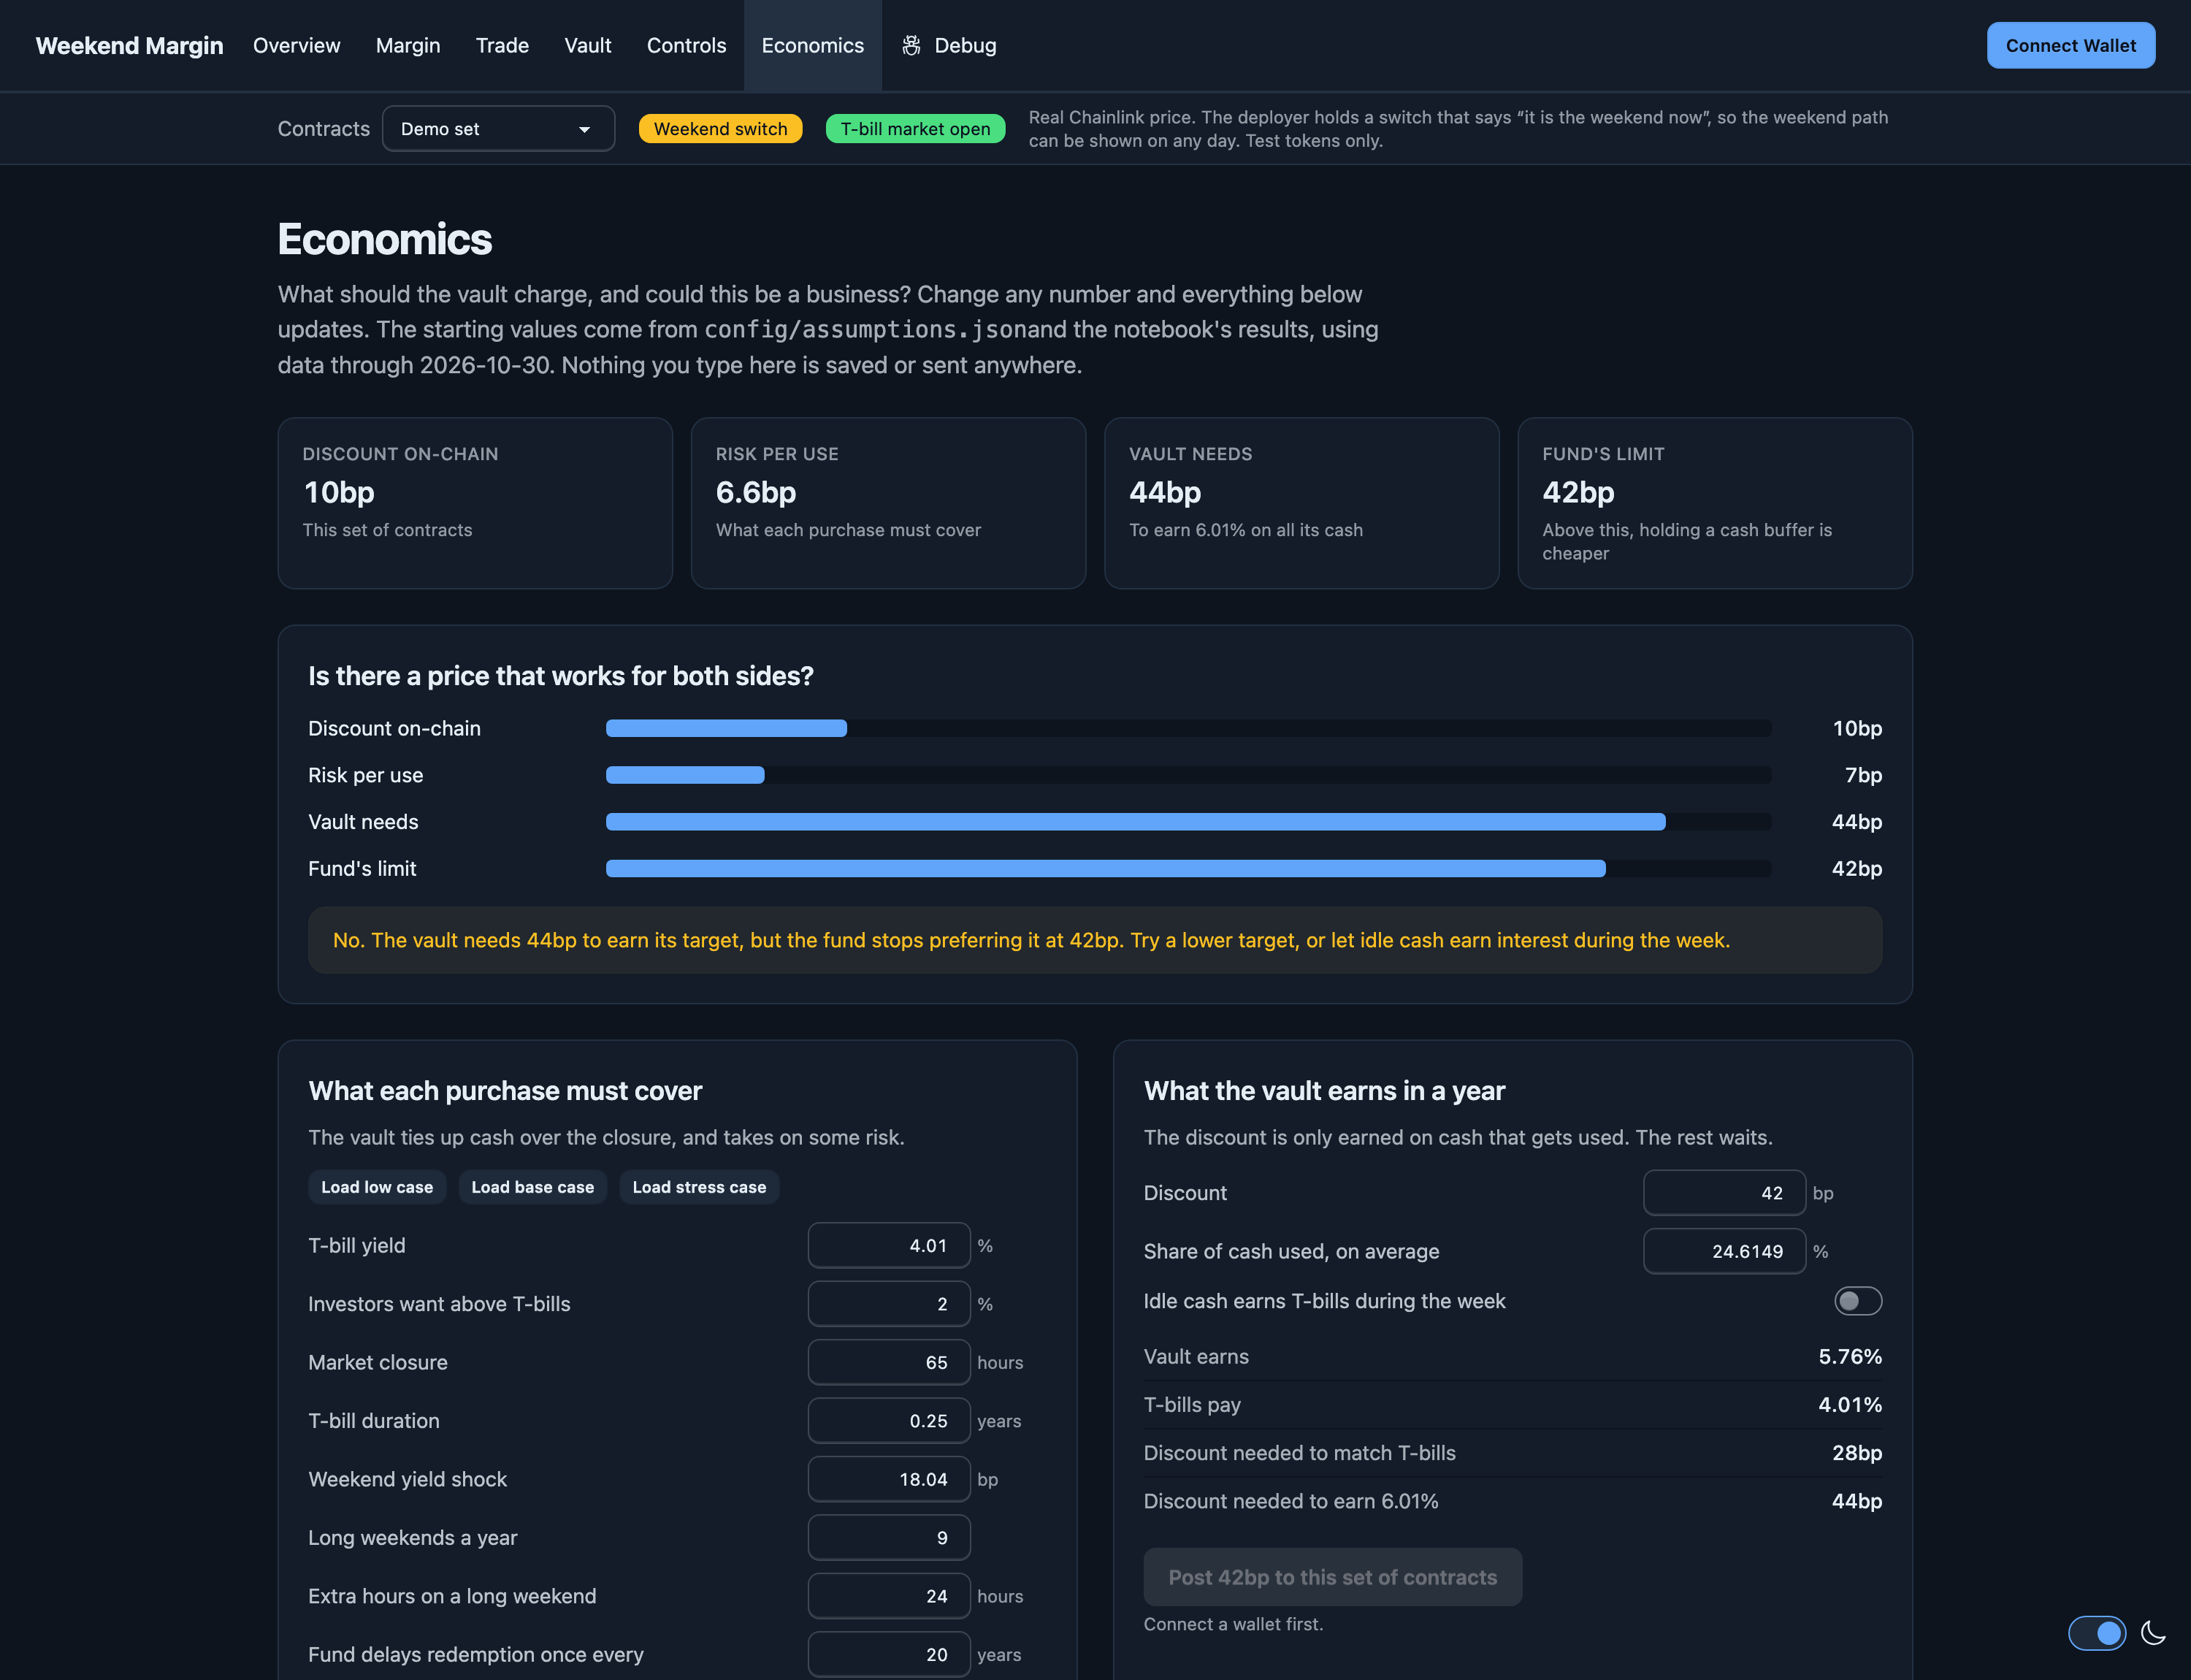
\includegraphics[width=\textwidth]{figures/screens/app_economics.png}
\caption{Economics. The whole pricing model from \S\ref{sec:vaulteconomics}, live and editable. Change
any input and the verdict recomputes — here it correctly reports that at a 2\% hurdle the vault needs
44bp while the fund stops paying at 42bp, so no deal exists. The result can be copied straight back
into \texttt{config/assumptions.json}.}
\end{figure}

\clearpage

%====================== 4. FINANCIAL ANALYSIS ======================
\section{Financial analysis}\label{sec:finance}

Most of this section comes from \texttt{docs/analysis.ipynb}. It runs end to end in about a minute,
and \textbf{no number is typed into a cell}: every judgement call lives in
\texttt{config/assumptions.json} and every contract setting in \texttt{config/protocol.json}, so a
reader who disagrees with us can change one file and rerun. The charts below are written straight to
\texttt{docs/figures/} by the notebook. Two parts come from elsewhere: the historical stress weekends
in \S\ref{sec:regimes} are written by \texttt{docs/stress\_weekends.py} from the same cached data with
the notebook's conventions, and the break points in \S\ref{sec:breaks} were derived in the companion
document \texttt{docs/pricing-and-risk.pdf}. Each section says so.

\subsection{Method and data}

\begin{center}
\small
\begin{tabular}{@{}p{3.4cm}p{3.2cm}p{3.0cm}p{5.4cm}@{}}
\toprule
\textbf{Series} & \textbf{Source} & \textbf{Coverage} & \textbf{Used for} \\
\midrule
BTC/USD hourly & Coinbase Exchange, \texttt{BTC-USD} & 2021-01-01 to 2026-10-30, 51,083 hours (13 filled) & Hedge backtest, closure moves, liquidation, regime stress \\
BTC perp funding, hourly & Deribit \texttt{BTC-PERPETUAL}, \texttt{interest\_1h} & matched to the above & Funding realism and the hedge's carry \\
3-month T-bill yield & FRED \texttt{DTB3}, daily & 2015-01-02 to 2026-10-28, 2,957 obs (3,085 rows, holidays blank) & The yield $y=4.01\%$ and weekend yield shocks \\
Live contract reads & Our own Sepolia deployment & 28 values at block \reconBlock{} & Reconciliation (\S\ref{sec:reconcile}) \\
\bottomrule
\end{tabular}
\end{center}

\note{All four series are cached in \texttt{docs/data/}, so only the reconciliation section touches
the network. The brief names BitMEX for funding data; its API returns HTTP 403 from our US network,
so we used Deribit and checked it against itself — the rolling 8-hour sum of \texttt{interest\_1h}
has correlation 0.9997 with Deribit's published \texttt{interest\_8h}.}

\subsubsection*{The position every number refers to}

\cbox{\textbf{The reference trade.} A fund owns 1 BTC bought at \$77,853.66. It shorts 1 BTC of perp
with \textbf{\$30,000 of sBILL} as margin — \textbf{2.60$\times$ leverage}. The counterparty is long
1 BTC with \$30,000 of tUSDC. Holding period 30 days. This is exactly the position the demo opened on
Sepolia, so the analysis and the chain describe the same thing.}

\subsection{Hedged versus unhedged P\&L}\label{sec:hedged}

\[
\text{Hedged P\&L} \;=\; \underbrace{(P_1-P_0)}_{\text{spot}} \;+\; \underbrace{-(P_{\text{exit}}-P_0)}_{\text{perp}}
\;+\; \text{funding} \;+\; \text{sBILL interest} \;-\; \text{vault cost}
\]

with funding $=$ rate $\times$ average notional (positive means longs pay shorts; the rate is the
median month's, 0.32\% of notional, about 3.8\% a year), interest $=$ sBILL balance
$\times\,4\%\times$ days$/365$ on a balance that shrinks by half the loss as sBILL is sold to pay
it, and vault cost $=$ 10bp $\times$ loss $\times\,65/168$, the
share of the week the T-bill market is shut.

\begin{figure}[h!]\centering
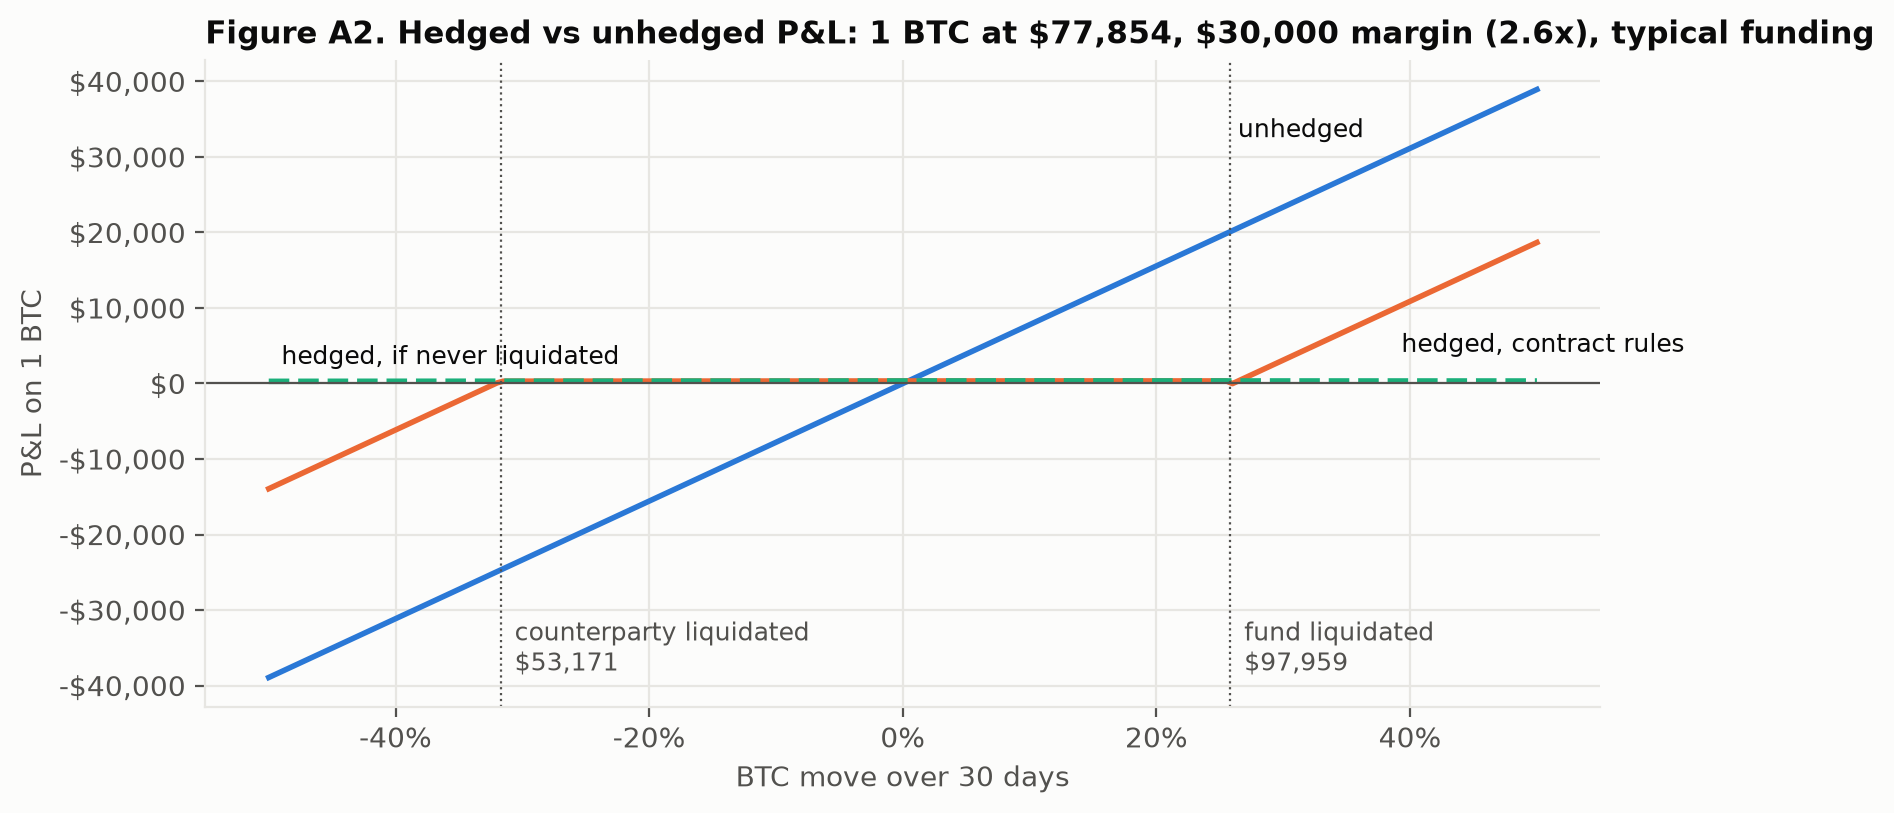
\includegraphics[width=0.96\textwidth]{figures/A2_hedged_vs_unhedged.png}
\caption{Hedged versus unhedged profit and loss across Bitcoin price scenarios, at the demo's
2.60$\times$ leverage. The flat middle is the hedge working. The two cliffs are liquidation.}
\end{figure}

\textbf{What the chart says, in three findings.}

\begin{enumerate}
  \item \textbf{Between $-32\%$ and $+26\%$ the result is flat}, at about \textbf{\$343 a month} per
  BTC. The parts, at a $+10\%$ move: spot $+\$7{,}785.37$, perp $-\$7{,}785.37$, funding
  $+\$260.93$, sBILL interest $+\$85.83$, vault cost $-\$3.01$. The hedge removes the price and
  leaves the carry, which is the purpose of the hedge.
  \item \textbf{Outside that range the fund is not hedged at all}, and the apparent upside in the
  chart is misleading, because the result is path-dependent. If Bitcoin reaches \$97,959 the short is
  liquidated; if it then
  returns to \$77,854, the fund is down \textbf{\$20,595} on the perp with nothing on the spot side
  to offset it.
  \item \textbf{Leverage decides the outcome.} Over 2,099 rolling 30-day windows, hedge effectiveness
  ($1 - \text{hedged variance}/\text{unhedged variance}$) is \textbf{97\% at 2$\times$, 92\% at
  2.6$\times$, 60\% at 4$\times$ and 34\% at 4.9$\times$}. Unhedged, those same windows have mean
  $+2.6\%$, standard deviation $16.9\%$ and a worst case of $-43.1\%$.
\end{enumerate}

\note{Two caveats. The backtest never tops up margin and never re-hedges after a liquidation,
which a real fund would do, so it is pessimistic. And ignore the ``mean hedged'' column when
comparing leverage: it \emph{rises} with leverage only because Bitcoin went up over the sample, so a
fund liquidated out of its short kept the gain. Read the standard deviation and the worst case.}

\subsubsection*{Unrealized P\&L, and where to read it on-chain}

The contract exposes unrealized profit and loss directly as
\texttt{unsettledPnl(account, price)}: the mark-to-market gain on an open position that has not yet
been settled in cash. At the moment of the reconciliation read, with Bitcoin at \$\reconBtc{} and
trade 1 last settled at \$78,462.47 (the keeper's settlement in \S\ref{sec:liverun}):
% UPDATE AFTER THE VIDEO: if trade 1 is settled again, the last-settled price above changes. Read it
% from the trade table on the site or from the Settled event, and update it here.

\begin{center}
\footnotesize
\begin{tabular}{@{}p{5.0cm}rr@{}}
\toprule
& \textbf{Model} & \textbf{Read from the chain} \\
\midrule
Trade 1, long's unrealized P\&L & $-\$\liveLongPnl$ & $-\$\liveLongPnl$ \\
Trade 1, short's unrealized P\&L & $+\$\liveLongPnl$ & $+\$\liveLongPnl$ \\
Fund A, margin value after haircut & \$\liveMarginValue & \$\liveMarginValue \\
Fund A, equity & \$\liveEquity & \$\liveEquity \\
Fund A, maintenance margin & \$\liveMaintenance & \$\liveMaintenance \\
Fund A, initial margin & \$\liveInitial & \$\liveInitial \\
\bottomrule
\end{tabular}
\end{center}

Unrealized P\&L is exactly zero-sum between the two sides, as a bilateral design requires, and the
fund's equity of \$\liveEquityRounded{} sits well above its \$\liveMaintenanceRounded{} maintenance
requirement. The
\textbf{strategy} this implies is stated in \S\ref{sec:pnlstrategy}.

\subsection{Funding}\label{sec:funding}

\begin{figure}[h!]\centering
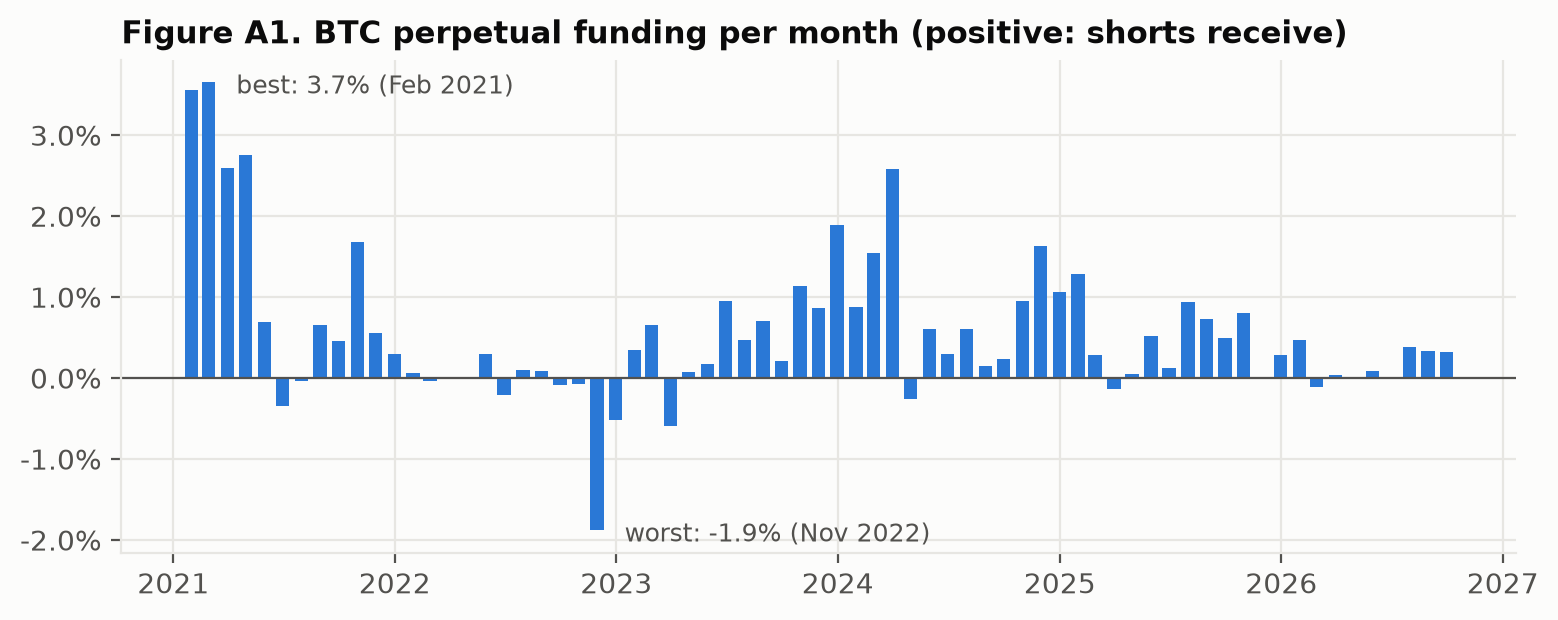
\includegraphics[width=0.94\textwidth]{figures/A1_monthly_funding.png}
\caption{Monthly funding on a 1 BTC perpetual, from Deribit hourly rates. Positive means the short
is paid.}
\end{figure}

\begin{center}
\small
\begin{tabular}{@{}p{8.2cm}p{7.0cm}@{}}
\toprule
\textbf{Measurement} & \textbf{Result} \\
\midrule
Mean funding rate over the sample & \textbf{6.6\% a year}, paid by longs to shorts \\
Months in which the short \emph{pays} & \textbf{20\%} \\
Worst month for a short & $-1.9\%$, November 2022 \\
Largest hourly rate ever observed & \textbf{0.0609\%} per hour \\
The contract's hard cap & 0.1\% per hour --- \textbf{never reached in 51,083 hours of data} \\
\bottomrule
\end{tabular}
\end{center}

So funding is a \emph{real} risk and a \emph{small} one next to price. A short hedger is paid about
two thirds of the time, and the contract's cap sits roughly 1.6$\times$ above anything the market has
produced in six years — tight enough to constrain an owner, loose enough never to block a legitimate
rate.

\subsection{The liquidation price}\label{sec:liq}

With $D$ the deposit, $h = 1 - \text{haircut}$ (so $h=1$ for tUSDC), $m=10\%$ the maintenance margin,
and $P_0$ the entry price, an account is liquidated when what remains after settlement and the
haircut falls below $m$ times the notional:

\[
\text{Short:}\quad h\,(D - (P-P_0)) = m P \;\Longrightarrow\; P_{\text{liq}} = \frac{h\,(D+P_0)}{m+h}
\qquad
\text{Long:}\quad P_{\text{liq}} = \frac{h\,(P_0-D)}{h-m}
\]

\begin{center}
\small
\begin{tabular}{@{}p{4.4cm}rrp{5.0cm}@{}}
\toprule
\textbf{Position} & \textbf{Liquidated at} & \textbf{BTC move} & \textbf{Note} \\
\midrule
Fund's short, 2.60$\times$, sBILL margin & \$97{,}959 & $+25.8\%$ & The demo's actual position \\
Counterparty's long, 2.60$\times$, tUSDC & \$53{,}171 & $-31.7\%$ & \\
\bottomrule
\end{tabular}
\end{center}

\begin{center}
\small
\begin{tabular}{@{}p{5.2cm}rp{7.2cm}@{}}
\toprule
\textbf{Margin posted as} & \textbf{Max leverage} & \textbf{Why} \\
\midrule
tUSDC margin & $5.00\times$ & The 20\% initial margin \\
sBILL, market open (1\% haircut) & $4.95\times$ & \\
sBILL, market closed (3\% haircut) & $4.85\times$ & \\
\textbf{10$\times$} & \textbf{cannot open} & It would already be below maintenance at entry \\
\bottomrule
\end{tabular}
\end{center}

Two results worth keeping. \textbf{The weekend haircut barely matters} — switching from 1\% to 3\%
moves the liquidation price by about \$185 on a figure near \$98,000, or 0.19\%, and costs a tenth of
a turn of leverage. \textbf{The vault discount matters even less}: \$18 at the demo's size. Both
buffers are close to free, which is the strongest argument for keeping them.

\cbox{\textbf{The finding that changed how we think about this product.} The 20\% initial margin is
about right for \emph{trading} and too loose for a month-long \emph{hedge}. With no top-ups, a
position at 4.9$\times$ has roughly a 20\% chance of liquidation within a week and about 55\% within
30 days; at the demo's 2.6$\times$ it is 14\% over 30 days. A liquidated hedge is worse than no
hedge, because the fund discovers it is naked at exactly the moment it most needed cover. A hedger
should sit near 2--2.6$\times$ or plan to add margin.}

\begin{figure}[h!]\centering
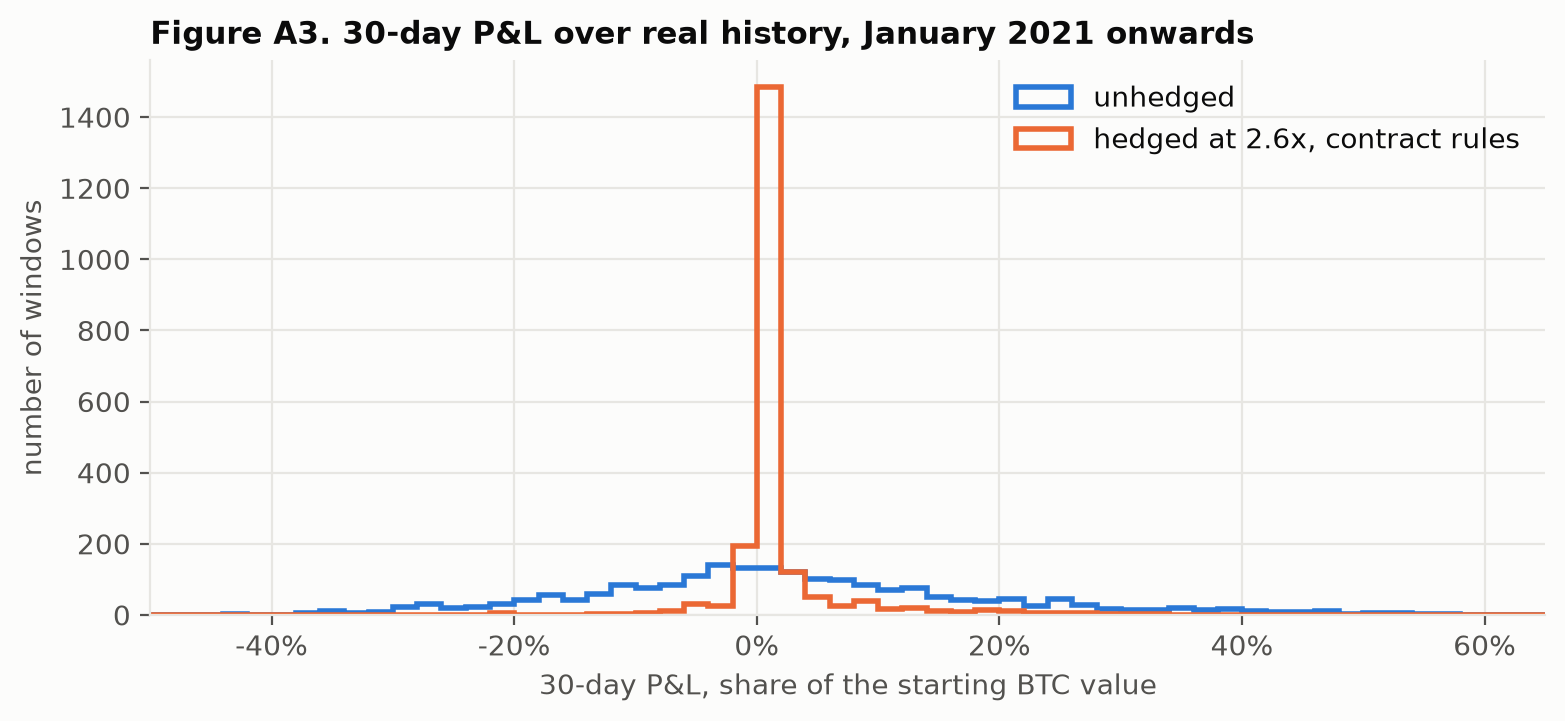
\includegraphics[width=0.94\textwidth]{figures/A3_hedge_backtest.png}
\caption{Rolling 30-day backtest across 2,099 windows: hedged versus unhedged outcomes by leverage.}
\end{figure}

\subsection{Is a weekend actually more dangerous?}\label{sec:weekendrisk}

We expected yes. The data says no.

\begin{center}
\small
\begin{tabular}{@{}p{6.6cm}rr@{}}
\toprule
& \textbf{Inside closures} & \textbf{Outside closures} \\
\midrule
Hourly volatility & \textbf{0.523\%} & \textbf{0.680\%} \\
\bottomrule
\end{tabular}
\end{center}

\begin{center}
\small
\begin{tabular}{@{}p{8.4cm}r@{}}
\toprule
\textbf{65-hour closure, 304 weekends since 2021} & \\
\midrule
99th-percentile adverse excursion within a closure, against a short (price up) & $+13.47\%$ \\
99th-percentile adverse excursion within a closure, against a long (price down) & $-14.42\%$ \\
99th-percentile Friday-to-Monday net move, up / down & $+11.10\%$ / $-12.97\%$ \\
Worst closure in the sample & $20.41\%$ \\
Fitted growth of volatility with horizon (exponent) & 0.493 \quad\note{(square-root rule says 0.5)} \\
Weekend-to-overnight volatility ratio & 1.66 \quad\note{(square-root rule predicts 1.96)} \\
\bottomrule
\end{tabular}
\end{center}

\begin{figure}[h!]\centering
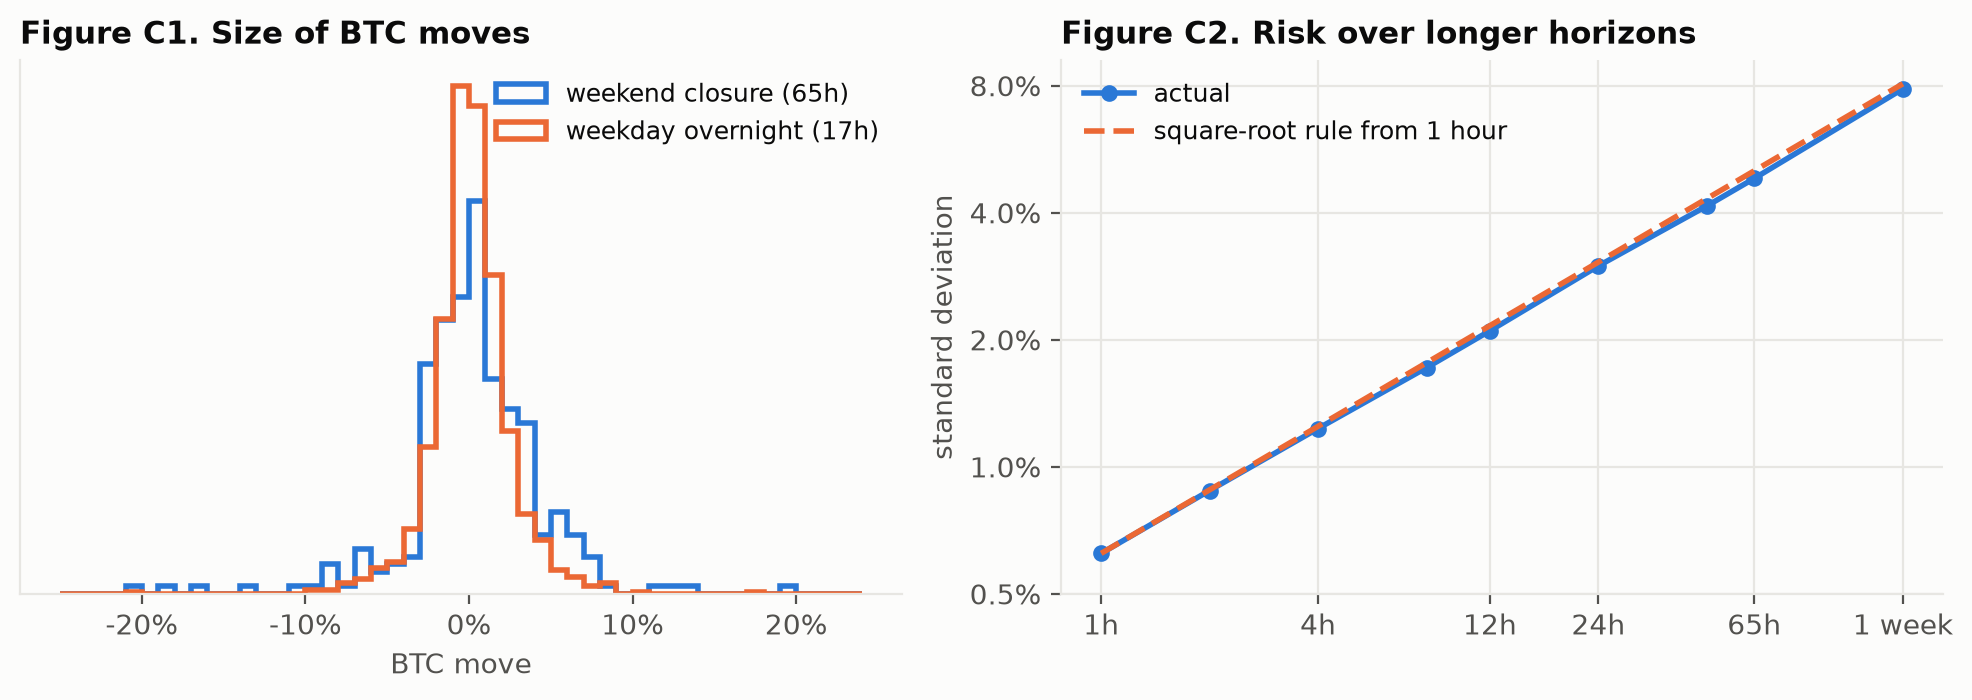
\includegraphics[width=0.96\textwidth]{figures/C_weekend_risk.png}
\caption{Weekend closures against matched weekday windows. Per hour, closures are calmer; they are
dangerous because they are long and because the collateral cannot be sold.}
\end{figure}

\note{An adverse excursion is the largest loss reached at any hourly settlement during the closure,
which is what settlement actually charges and what the vault has to fund. The Friday-to-Monday net
move is smaller because prices partly recover before Monday. The vault sizing below uses the
excursion.}

\textbf{Three consequences.}

\begin{itemize}
  \item \textbf{The weekend problem is a plumbing problem, not a volatility problem.} Bitcoin does
  not misbehave at weekends. The T-bill market being shut is the entire issue, which is why a vault,
  rather than a larger margin requirement, is the right response.
  \item \textbf{The square-root rule overstates the tail.} Over every 65-hour window in the sample,
  the 99th percentile of the absolute move is 15.9\%, against 19.3\% if the one-hour figure is scaled
  by the square root of time. Using the rule would have made us hold about 20\% more vault capital
  than the data requires.
  \item \textbf{Maintenance margin holds up well.} A 10\% margin would have been breached by a
  single-hour move in only \textbf{2 of 51,083 hours}, and by a two-hour move in 4 — all in January
  and May 2021. Two hours is the relevant window because it is the oldest price the contract accepts.
  In those rare cases an account sitting exactly at maintenance could underpay the winner, because
  there is no insurance fund.
\end{itemize}

\note{The sample is small where it matters most: 304 weekends means a 99\% figure rests on about
three observations. The 90\% bootstrap interval is $7.7\%$--$13.9\%$ for rises and
$8.7\%$--$18.3\%$ for falls, so read these as ranges, not points.}

\subsection{What should the vault charge?}\label{sec:vaulteconomics}

This is the question the proposal feedback asked. The answer has two parts that give very different
numbers, and the distinction between them is the most useful result in our analysis.

\subsubsection*{Part 1 --- the cost of each use}

Per dollar the vault actually deploys over a closure of $h$ hours:

\[
\underbrace{\frac{(y+\pi)h}{8760}}_{\text{gross carry}}
\;-\;\underbrace{\frac{yh}{8760}}_{\text{the sBILL keeps accruing}}
\;+\;\underbrace{D\cdot\Delta y}_{\text{T-bill price risk}}
\;+\;\underbrace{p_{\ell}\frac{(y+\pi)h_{\text{extra}}}{8760}}_{\text{long-weekend risk}}
\;=\;\text{required discount}
\]

with $y$ the T-bill yield, $\pi$ the hurdle premium vault depositors require above T-bills, $D$ the
collateral's duration, $\Delta y$ the weekend yield shock, and $p_\ell$ the chance of a Monday
holiday. Note that the first two terms largely cancel: the vault's capital must earn $y+\pi$, but the
sBILL it is holding is itself earning $y$, so only the premium has to come out of the discount. The
notebook adds one more small term: an allowance of about 0.3bp for a redemption gate (one gate in
twenty years, costing 3\%). The companion document omits it, which is why its base case is 6.3bp
where the notebook's, used below, is 6.6bp.

$\Delta y$ is an \textbf{empirical percentile, not a standard deviation}, and that choice is
deliberate. Weekend yield moves are far from normal: a normal distribution expects 0.04 weekends
beyond $4\sigma$ in a sample this size and we observe nine, and June 2022 is an $8.4\sigma$ move
(both computed in \texttt{docs/pricing-and-risk.pdf}). We read the quantile straight off 597
observed weekends instead.

\begin{center}
\small
\begin{tabular}{@{}lrr@{}}
\toprule
\textbf{Weekend yield move, 597 weekends since 2015} & \textbf{Yield} & \textbf{Price impact at $D=0.25$} \\
\midrule
Median & 2bp & 0.50bp \\
95th percentile & 10bp & 2.50bp \\
99th percentile & 18.04bp & 4.51bp \\
Largest ever, 2022-06-10 & 35bp & 8.75bp \\
\bottomrule
\end{tabular}
\end{center}

\begin{center}
\small
\begin{tabular}{@{}lrrrr@{}}
\toprule
\textbf{Case} & \textbf{Hurdle} & \textbf{Duration} & \textbf{Shock} & \textbf{Discount required} \\
\midrule
Low & 4.01\% & 1 month & 10bp & 1.3bp \\
\textbf{Base} & 6.01\% & 3 months & 18bp & \textbf{6.6bp} \\
Stress & 9.01\% & 3 months & 35bp & 13.2bp \\
\bottomrule
\end{tabular}
\end{center}

\textbf{The contract charges 10bp, which is 1.5$\times$ the base requirement.} The largest single
component is T-bill \emph{price} risk — 4.51 of the 6.6bp. The most important thing our fee prices is
the risk that interest rates move while the vault holds the paper.

\subsubsection*{Part 2 --- the cost of cash that waits, which is where 10bp fails}

The vault must hold enough cash for a bad weekend. Most weekends use almost none of it. Measuring
each weekend's draw from the real hourly price path — the \emph{largest} loss reached at any hourly
settlement, not the final one, because settlement is continuous:

\begin{center}
\small
\begin{tabular}{@{}p{8.8cm}r@{}}
\toprule
A hedging fund sells, per weekend, on average & \textbf{2.50\% of notional} \\
\quad median & 1.80\% \\
\quad largest & 19.9\% \\
\midrule
Cash needed to cover 99\% of weekends --- shorts only & 13.47\% of notional \\
Cash needed to cover 99\% of weekends --- longs only & 14.42\% of notional \\
\textbf{Cash needed, one pool serving both directions} & \textbf{19.69\% of notional} \\
\quad \note{pooling saves \textbf{29\%} of the capital, the largest single efficiency in the design} & \\
\midrule
Average utilisation at that sizing --- shorts only & 18.29\% \\
Average utilisation at that sizing --- both directions & 24.61\% \\
\bottomrule
\end{tabular}
\end{center}

\begin{figure}[h!]\centering
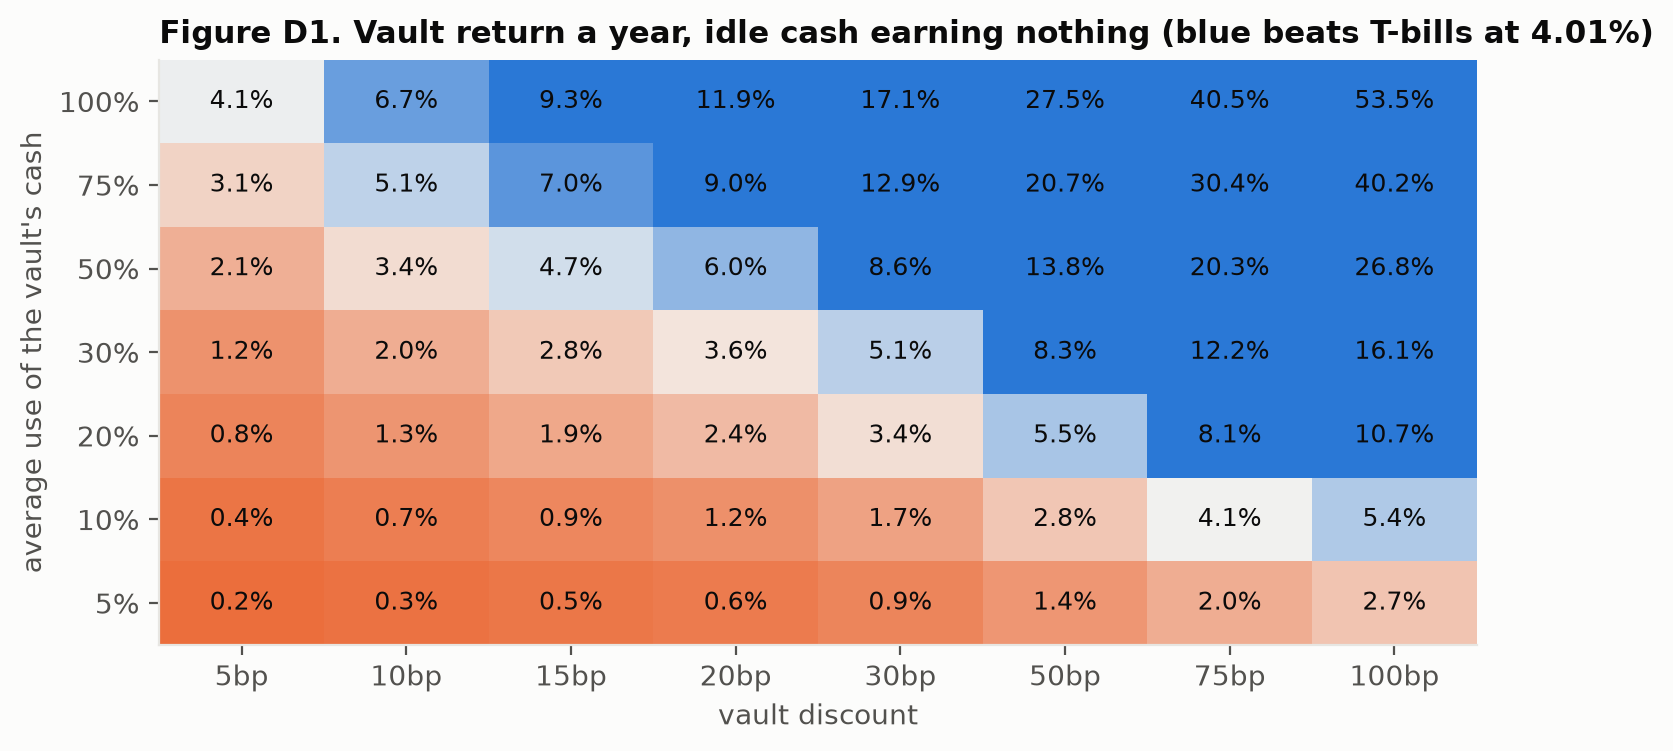
\includegraphics[width=0.94\textwidth]{figures/D1_vault_return.png}
\caption{What the vault actually earns, per year, as a function of the discount it charges — against
the 4.01\% it could have earned simply holding T-bills.}
\end{figure}

\cbox{\textbf{The main finding, which goes against our own deployed setting.} At the deployed
\textbf{10bp the vault earns 1.2--1.7\% a year against 4.01\% on T-bills}. It loses to its own
alternative. The cause is \emph{not} the weekend: 10bp covers the 6.6bp cost of every use
comfortably. The cause is that three quarters of the vault's capital is idle waiting for a weekend
that mostly does not need it. A real vault needs \textbf{28bp to match T-bills and 44bp to earn
T-bills $+$ 2\%}, serving both directions from one pool.}

\textbf{Three things would fix it}, and they are the design roadmap:

\begin{enumerate}
  \item \textbf{Raise the discount.} Serving shorts only: 39bp to match T-bills, 60bp for
  T-bills $+$ 2\%. Serving both directions: 28bp and 44bp.
  \item \textbf{Serve both directions from one pool} — already true in our design, and worth 29\% of
  the capital.
  \item \textbf{Sweep idle cash into T-bills on business days.} With both directions plus a sweep the
  vault needs only \textbf{9bp} to match T-bills and 25bp for T-bills $+$ 2\%. Our contracts do not do
  this; it is the single highest-value extension.
\end{enumerate}

\textbf{What we did about it.} We left 10bp deployed, because the contracts are frozen, and we report
the result as it is. The discount is owner-adjustable up to 1\% without a redeploy, so the fix is one
transaction away, and the Economics page can post it.

\subsection{Is the fund better off? The price band}\label{sec:band}

The other side of the trade. Take a \$1,000,000 hedge at the demo's leverage (\$385,338 of margin)
and compare four ways to hold that margin for a year:

\begin{center}\small
\begin{tabular}{@{}p{5.4cm}p{9.8cm}@{}}
\toprule
1. All cash & income $=0$ \\
2. T-bills $+$ a cash buffer & income $= y\,(M - \text{buffer})$, buffer $=$ 99\% weekend move $\times$ notional \\
3. T-bills, sold every Friday & income $= y\,(M - \text{buffer}\times 65/168)$, and someone must trade every week \\
4. \textbf{All T-bills $+$ our vault} & income $= y\,M - \text{discount}\times\text{sBILL sold}$ \\
\bottomrule
\end{tabular}
\end{center}

\begin{center}
\small
\begin{tabular}{@{}p{8.6cm}rr@{}}
\toprule
\textbf{On a \$1m hedge, \$385,338 of margin} & \textbf{Return on margin} & \textbf{Income} \\
\midrule
All cash & 0.00\% & \$0 \\
T-bills $+$ cash buffer & 2.61\% & \$10{,}050 \\
\textbf{All T-bills $+$ the vault, at 10bp} & \textbf{3.67\%} & \textbf{\$14{,}150} \\
\bottomrule
\end{tabular}
\end{center}

The fund pays about \$1,300 a year in discounts (it routes roughly \$1,301,320 of sBILL through the
vault annually) to earn about \$15,450 of T-bill interest. That is the product in one line.

\begin{figure}[h!]\centering
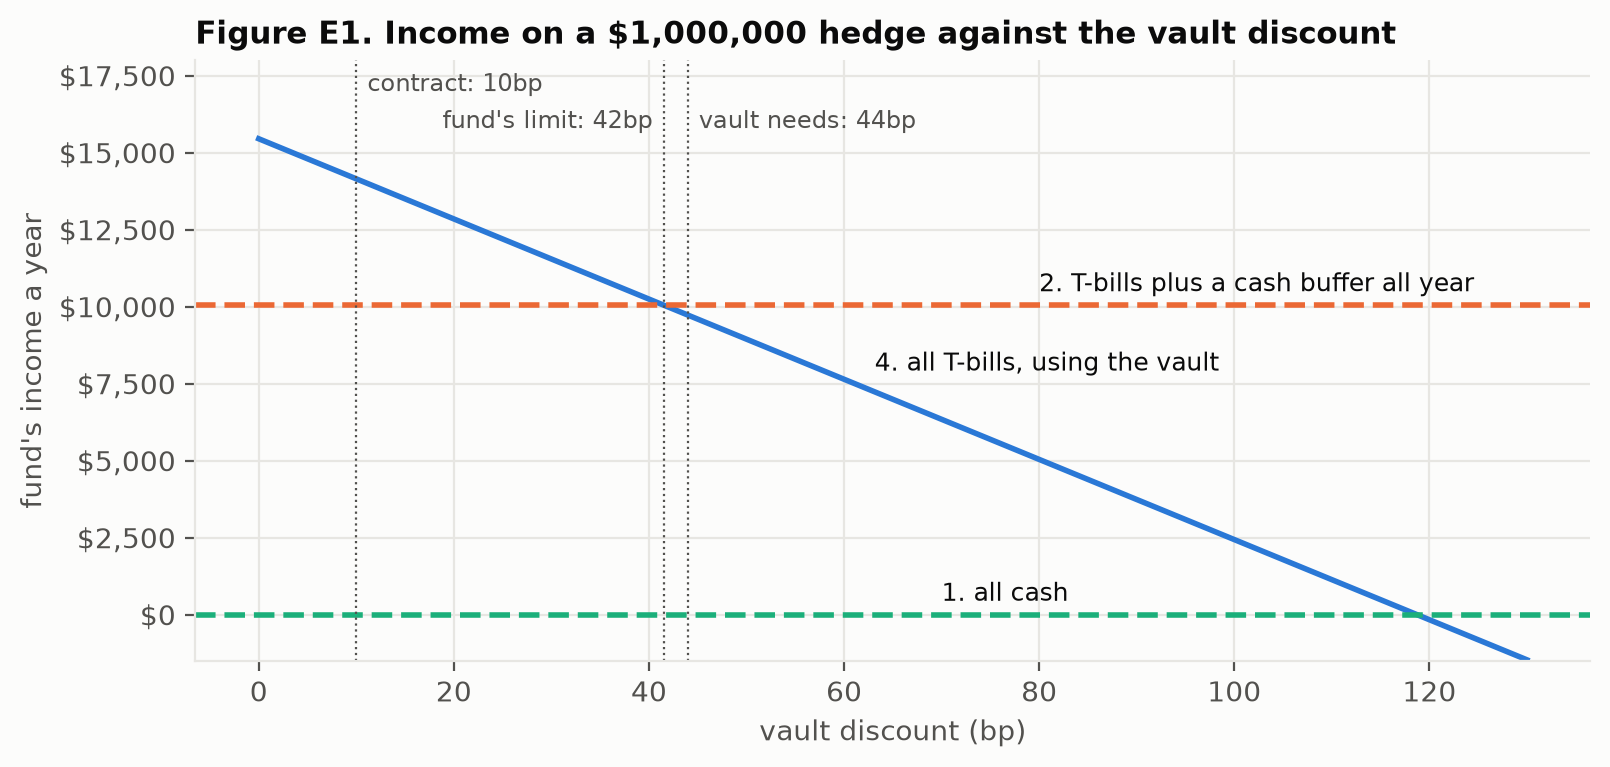
\includegraphics[width=0.94\textwidth]{figures/E1_fund_income_vs_discount.png}
\caption{The fund's income against the discount charged, with the vault's break-even lines. The two
constraints almost touch — which is the real finding.}
\end{figure}

\begin{center}
\small
\begin{tabular}{@{}p{10.0cm}r@{}}
\toprule
\textbf{Constraint} & \textbf{Discount (bp)} \\
\midrule
Vault must earn at least this to match T-bills (both directions, one pool) & 28 \\
Vault must earn at least this for T-bills $+$ 2\% & 44 \\
\textbf{Fund will pay at most this, against holding a cash buffer} & \textbf{42} \\
Fund will pay at most this, against selling T-bills every Friday & 16 \\
Fund will pay at most this, against holding everything in cash & 119 \\
\bottomrule
\end{tabular}
\end{center}

\cbox{\textbf{A workable price exists between 28 and 42bp — and only against the cash-buffer
alternative.} Against a fund disciplined enough to sell T-bills every Friday there is no overlap at
all. This is a narrow business, and we say so. It also requires rates: at 2021's 0.05\%, a user of
this product would have \emph{lost} about \$2,222 a year on a \$1m hedge.}

\subsection{Stress: what history would have done to us}\label{sec:regimes}

For each crisis we take the worst 65-hour closure in the surrounding window, measured as the adverse
excursion from Friday 4pm ET on settled hourly closes. Excursion, not the Friday-to-Monday net move,
because settlement is hourly: the loser pays as the price goes against it, and a later recovery does
not hand back collateral already sold.

The table is written by \texttt{docs/stress\_weekends.py} from the cached Coinbase series, with the
notebook's conventions (hourly settlement at the candle open, Friday 4pm New York time, 65 hours), so
it agrees with the notebook's table of the busiest weekends (Section~C). Each row is the worst
closure within three weeks of the event, and the script checks that. The companion document's
version of this table uses a slightly different convention (hourly closes from Friday 20:00 UTC) and
takes each named event's own weekend, so its figures differ by small amounts and, for October 2025,
it shows the 24th where this rule selects the 10th, the weekend of the figure below. Its conclusions
hold under both; where the two differ, this table is the one to cite.

\begin{center}
\small
\stressTable
\end{center}

\textbf{Read that last column carefully, because it is the single most important risk number in this
project.} A vault sized at the 95th percentile of that excursion distribution holds
\$\stressVaultNinetyFive{} per \$1m of notional, and
\textbf{\stressExceed{} of the seven crises exceed it}. When the vault empties, \texttt{settle()} reverts and
settlement waits for Monday — a safe failure, but a failure, and exactly in the weekends the product
exists for.

\cbox{\textbf{The binding constraint is capital, not price.} In every one of those seven weekends the
10bp fee was comfortable; in four of them the \emph{cash} was not. That moves the open design
question from ``is 10bp enough?'' — which we can now answer yes, for each use — to ``how much capital
stands behind it?'', which is where the remaining work belongs. We size at the 99th percentile for
this reason, and we would go higher.}

\textbf{Does the position survive?} By the same script, at the demo's 2.6$\times$ nothing is
liquidated in any of the seven regimes. At 4$\times$ the June 2022 and yen-unwind longs go, and the SVB short goes. At the
4.85$\times$ maximum the 2021 mining-ban long goes too. \textbf{The demo is safe because it is
conservatively levered, not because the parameters are strong}, which the Sepolia run alone would not
show.

\begin{figure}[h!]\centering
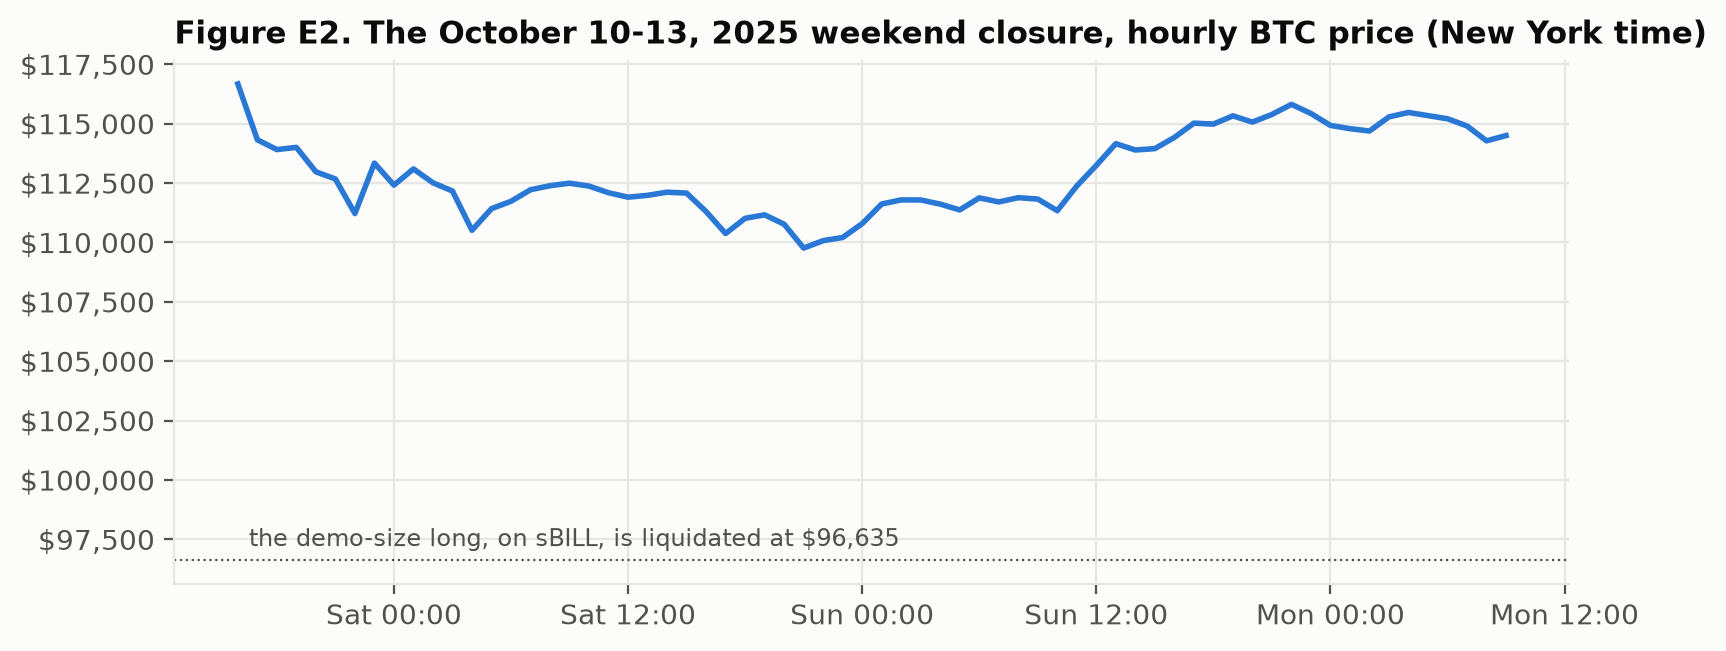
\includegraphics[width=0.94\textwidth]{figures/E2_oct_2025_stress.png}
\caption{October 10--13, 2025, the most recent real stress weekend. On Coinbase hourly data Bitcoin
fell 5.9\% from the Friday 4pm ET price of \$116,673 (8.3\% at the lowest trade). The demo's long
side would have sold \$6,908--\$9,673 to the vault — at most 19\% of the \$50,000 demo vault — and
would not have been liquidated. Other assets and other venues fell much further that weekend, which
BTC-only, single-exchange data cannot show.}
\end{figure}

\subsection{Reconciling the model with the chain}\label{sec:reconcile}

\textbf{The brief requires at least one model number to match a result on Sepolia. We matched 28, to
the wei.}

Contracts do whole-number arithmetic with 18 decimals, so the notebook uses Python integers and
rounds exactly as the contract rounds. A ``match'' means equal to the last of 18 decimal places, and
the cell raises an error rather than reporting a near miss.

\begin{center}
\small
\begin{tabular}{@{}p{7.2cm}rp{5.4cm}@{}}
\toprule
\textbf{Read at block \reconBlock, \reconTime} & \textbf{Compared} & \textbf{Result} \\
\midrule
Settlements (amount due and funding) & 8 & all match \\
Vault purchase (price and sBILL taken) & 2 & all match \\
Vault redemption (cash received and profit) & 3 & all match \\
sBILL subscriptions (NAV and shares minted) & 4 & all match \\
Live state (NAV, purchase price, funding total) & 4 & all match \\
Account health (collateral, equity, both margin levels) & 4 & all match \\
Unrealized P\&L, both sides of trade 1 & 2 & all match \\
Liquidation reward, stress set & 1 & match \\
\midrule
\textbf{Total} & \textbf{28} & \textbf{28 match, difference 0} \\
\bottomrule
\end{tabular}
\end{center}

Two of these deserve a note. The \textbf{funding check} rebuilds the contract's running total from
the posted rates alone, so it would catch any error in how a rate change is applied — it is a test of
the fix in \S\ref{sec:design}, not just of a number. And the \textbf{liquidation check} does not only
compare the reward: \texttt{demoLiquidation.ts} computes the liquidation price from the formula in
\S\ref{sec:liq}, then shows the contract refusing at 0.1\% below it and accepting at 0.1\% above it.

The full table is in \texttt{docs/data/sepolia\_reconciliation.csv} and reproduced in
Appendix~\ref{app:recon}. On a tougher local rehearsal — repeated demos, rate changes, a discount
change and a liquidation — all 51 comparisons matched too.

\subsection{Where each assumption breaks}\label{sec:breaks}

Stating assumptions is necessary but not sufficient. The useful exercise is to solve each one for the
value at which our conclusion stops holding, and then ask whether history has already reached it.
The thresholds below were derived in \texttt{docs/pricing-and-risk.pdf} from the four-term
decomposition of \S\ref{sec:vaulteconomics}, without the 0.3bp gate allowance; the notebook's
sensitivity grids (Section~C) show the same pattern.

\begin{center}
\small
\begin{tabular}{@{}p{4.0cm}p{1.8cm}p{2.2cm}p{1.8cm}p{4.4cm}@{}}
\toprule
\textbf{Input} & \textbf{Base} & \textbf{Breaks above} & \textbf{Headroom} & \textbf{Reached in history?} \\
\midrule
Weekend yield shock & 18bp & \textbf{32.9bp} & $1.8\times$ & \textbf{Yes --- 35bp, June 2022} \\
Collateral duration & 0.25 yr & \textbf{0.456 yr} & $1.8\times$ & Immediately, on 6-month paper \\
Closure length & 65 h & 228 h & $2.0\times$ & No. Longest ever is 113 h (Thanksgiving) \\
Hurdle premium & 2.0\% & 6.7\% & $3.4\times$ & Not observable \\
\bottomrule
\end{tabular}
\end{center}

\textbf{Two of the four matter and two do not.} Closure length and the hurdle premium have two to
three times the headroom they need, so a reader can argue about them freely without changing a
conclusion. The yield shock has already been breached once. And \textbf{duration is the tightest
assumption in the model} — and the only one that is about our own collateral rather than about the
world, which makes it the one we can actually do something about.

\begin{center}
\small
\begin{tabular}{@{}p{4.0cm}p{2.1cm}p{1.6cm}p{5.6cm}@{}}
\toprule
\textbf{Collateral} & \textbf{Loses money above} & \textbf{Worst ever} & \textbf{Verdict} \\
\midrule
3-month bill (our assumption) & 51.9bp & 35bp & $1.5\times$ headroom \\
6-month bill & 26.0bp & 35bp & \textbf{Has already happened} \\
1-year note & 13.0bp & 35bp & \textbf{Happens regularly} --- the 99th percentile is already 18bp \\
\bottomrule
\end{tabular}
\end{center}

The design implication is concrete and belongs in the contract rather than in a spreadsheet:
\textbf{the vault should accept only short-dated collateral, and that limit should be enforced, not
assumed.}

\note{\textbf{What ``breaks'' means.} Two thresholds are easy to collapse into one and should not be.
Missing the hurdle (depositors earn less than they required) happens at 32.9bp and \emph{has}
occurred once, June 2022. Losing principal (the ERC-4626 share price actually falls) needs 51.9bp and
has never occurred. On \$100,000 routed through the vault, June 2022 would have left it \$5.19 short
of what it promised, having still made \$42.25. A small shortfall, not a loss of principal.}

\subsection{Three risks the fee does not properly price}\label{sec:mockgap}

Three risks are left out of the fee, or covered only by a nominal allowance, so that a reader can see
exactly what it covers and what it does not.

\begin{enumerate}
  \item \textbf{Our own token cannot express the risk that dominates its fee.} \texttt{SBill.nav()}
  grows purely on the clock, so rates cannot move it. T-bill price risk is 4.51 of the 6.6bp required
  discount — \textbf{72\% of the fee} — and it is a risk our deployment \emph{structurally cannot
  experience}. The 35bp spike of June 2022 would be invisible to us. We priced the asset the design
  calls for rather than the mock standing in for it, which is the right way round, but it means the
  largest component of our fee is one no unit test and no Sepolia transaction can exercise.
  \item \textbf{Redemption gates: a nominal allowance, not an estimate.} A tokenized fund can
  suspend redemptions, and our own \texttt{SBill} has the same shape of failure — \texttt{redeem()}
  pays from a reserve funded once after deployment. The notebook's base case allows about 0.3bp for
  this (one gate in twenty years, costing 3\%). The sector is about two years old and has never been
  stressed, so that frequency is a judgement rather than an estimate. The more useful statement is
  the threshold: \textbf{the fee stops clearing its hurdle if gates reach about one weekend in
  eighty}, roughly once every eighteen months.
  \item \textbf{The stablecoin leg, which is the largest exposure in the whole system.} The model
  prices 4.51bp of risk on paper the vault holds for 65 hours, and \textbf{zero} on the stablecoin it
  holds permanently. In March 2023 USDC traded at \$0.87 — \textbf{1,300bp}, more than two hundred
  times our entire risk budget, or 89 years of fee revenue on a \$1m book. It is also wrong-way: the
  vault holds the most cash during a crisis, and a crisis is when stablecoins depeg. The SVB weekend
  appears twice in this report for that reason — third-largest draw in \S\ref{sec:regimes}, and
  largest unpriced loss here. Circle's own stated trigger was that its wires had not settled before
  the weekend, which is the identical mechanism we built this system to address.
\end{enumerate}

\textbf{This is not a charge any fee absorbs; it is a position limit.} A production version would cap
the vault's idle balance, hold part of it in a second stablecoin, or accept the exposure explicitly
rather than silently.

\subsection{What we would change in the model}

\begin{enumerate}
  \item Cap collateral duration in the contract. The tightest assumption, currently unenforced.
  \item Cap or reserve against the stablecoin leg.
  \item Size the vault above the 95th percentile. Four of seven historical crises exhaust it.
  \item Emit signed profit and loss from \texttt{redeemInventory()} --- see \S\ref{sec:selffound}.
  \item Promote five judgement parameters out of notebook function defaults and into the settings
  cell, so a reader can disagree with them without reading code.
\end{enumerate}

%====================== 5. TESTING, SECURITY, GAS ======================
\section{Testing, security and gas}\label{sec:testing}

\subsection{The test suite}

One command, \texttt{yarn test}. \textbf{37 tests, all passing}, in about a second, across thirteen
groups. \textbf{25 of them expect a revert} — we tested what the contracts refuse at least as hard
as what they allow.

\begin{center}
\small
\begin{tabular}{@{}p{5.4cm}p{10.0cm}@{}}
\toprule
\textbf{Group} & \textbf{What it pins down} \\
\midrule
\texttt{MarketCalendar} (3) & Closed for exactly 65 hours, closes exactly at Friday 21:00 UTC, and reports itself as the real calendar rather than the demo one \\
\texttt{DemoCalendar} (1) & Only the operator can switch the weekend \\
\texttt{SBill} (2) & Accrues 4\% a year; \textbf{refuses to issue or redeem on a non-business day} \\
\texttt{WeekendVault} (4) & Only the owner changes the discount, within the hard limit, while the market is open; prices correctly after a change; refuses a starting discount above the cap; only sells cash to the clearinghouse, and the link cannot be changed twice \\
Weekend margin call (4) & \textbf{The headline path}: sells sBILL to the vault on Saturday, the vault profits on Monday; caps withdrawals while sBILL waits; refuses to redeem before the market reopens; reverts when the vault is short of cash \\
Weekday settlement (2) & Redeems with the fund at full NAV instead of using the vault \\
Price feed (3) & Rejects a price over 2 hours old, accepts one just under, rejects zero or negative \\
Margin rules (4) & Refuses an oversized offer; refuses a withdrawal that breaks margin; stops self-dealing; closes cleanly \\
Funding (4) & Charges hourly at the posted rate; \textbf{applies a new rate only from the moment it is posted}; adds up across a change; caps the rate and restricts it to the owner \\
Liquidation (5) & Pays the liquidator 0.5\%; works through the vault at a weekend; \textbf{underpays the winner rather than reverting} when a deposit runs out; \textbf{matches the liquidation-price formula}; refuses a healthy trade \\
Pause (1) & Stops new deposits and offers, but \textbf{never} settlement, withdrawals or closing \\
\textbf{Randomised invariant} (3) & Seeds 7, 42 and 2026: thousands of random settlements, and \textbf{no tUSDC or sBILL is ever created or destroyed} \\
Demo deployment (1) & A Thursday settlement routes through the vault once the operator flips the switch \\
\bottomrule
\end{tabular}
\end{center}

The three randomised runs are the ones we trust most. They do not check a number we chose; they
check that the books balance after arbitrary sequences of settlement, which is the property a
clearinghouse actually has to have.

\subsection{Slither}\label{sec:slither}

Slither 0.11.6, run against every contract with the same compiler as the deployment.
\textbf{26 findings on our own code. We fixed 4 and explain all 22 of the others, one by one, in
\texttt{docs/slither.md}. None is an exploitable bug.}

\begin{center}
\small
\begin{tabular}{@{}lrr@{}}
\toprule
\textbf{Severity} & \textbf{Before} & \textbf{After} \\
\midrule
High & 1 & 1 \quad\note{(a false positive, below)} \\
Medium & 9 & 8 \\
Low & 14 & 12 \\
Informational & 2 & 1 \\
\bottomrule
\end{tabular}
\end{center}

\subsubsection*{What we fixed}

\begin{center}
\small
\begin{tabular}{@{}p{3.6cm}p{5.2cm}p{6.4cm}@{}}
\toprule
\textbf{Finding} & \textbf{Where} & \textbf{The fix} \\
\midrule
\texttt{uninitialized-local} (Medium) & \texttt{liquidate}: \texttt{address account} declared empty and set in a branch & Rewrote so the check comes first and the variable is set once \\
\texttt{shadowing-local} (Low) $\times2$ & \texttt{maxWithdraw}, \texttt{maxRedeem}: a parameter named \texttt{owner} hid \texttt{owner()} & Renamed it \texttt{holder} \\
\texttt{unindexed-}\newline\texttt{event-address} (Info) & \texttt{ClearinghouseSet} & Made the address \texttt{indexed} \\
\bottomrule
\end{tabular}
\end{center}

We also reduced a \texttt{reentrancy-no-eth} finding by moving the trade's price, funding total and
timestamp updates \emph{before} any token movement in \texttt{\_settle}.

\subsubsection*{What we looked at and kept, with the reason}

\begin{center}
\small
\begin{tabular}{@{}p{3.1cm}p{3.6cm}p{8.5cm}@{}}
\toprule
\textbf{Finding} & \textbf{Where} & \textbf{Why it is fine} \\
\midrule
\texttt{weak-prng} (\textbf{High}) & \texttt{MarketCalendar.}\newline\texttt{secondsIntoWeek} & \textbf{False positive.} Slither sees \texttt{\%} applied to a timestamp and assumes someone is generating randomness. This is arithmetic to find the time of week. No randomness exists anywhere in the project \\
\texttt{reentrancy-no-eth} (Medium) $\times4$ & \texttt{closeTrade}, \texttt{liquidate}, \texttt{\_settle}, \texttt{\_collect} & Every entry point is \texttt{nonReentrant}; the callees are our own contracts, fixed at deployment; and the ERC-20s here have no transfer hooks, so no outside code can run mid-call. \textbf{We note the limit of that reasoning: against a production issuer whose token may have hooks or a blocklist, this needs revisiting} \\
\texttt{incorrect-equality} (Medium) $\times3$ & \texttt{shares == 0}, \texttt{amountDue == 0}, \texttt{tradeId == 0} & Each is a ``nothing to do'' check. Sending the vault one wei of sBILL only means it gets redeemed; a trade ID cannot be influenced from outside \\
\texttt{unused-return} (Medium) & \texttt{\_price} & Deliberate. \texttt{latestRoundData} returns five values and we check four. \texttt{startedAt} adds nothing once \texttt{updatedAt} is checked \\
\texttt{missing-zero-check} (Low) & \texttt{setClearinghouse} & Harmless: a zero address leaves the link unset and the owner can call again. It can never be changed once set \\
\texttt{reentrancy-events} (Low) & \texttt{redeemInventory} & The event is emitted after a call to sBILL, our own contract, and the inventory cost is already zeroed before that call \\
\texttt{timestamp} (Low) $\times10$ & NAV, funding, calendar, staleness, faucet & The system depends on the clock by design. A validator can move a block's time a few seconds; at 4\% a year that is a fraction of a cent \\
\texttt{solc-version} (Info) & \texttt{pragma \^{}0.8.20} & The pragma permits older compilers, but the project compiles with exactly 0.8.30, pinned in \texttt{hardhat.config.ts} \\
\bottomrule
\end{tabular}
\end{center}

\subsubsection*{What the scanner could not find}\label{sec:selffound}

This part matters most. A scanner looks for known code patterns; it cannot tell whether the finance
is right. Reading our own code found three things Slither missed, all now fixed:

\begin{enumerate}
  \item \textbf{Funding applied backwards in time} — on a trade left unsettled for 30 days, the owner
  could have charged 72\% of the position instantly. Fixed, with a test (\S\ref{sec:design}).
  \item \textbf{Nothing tied the discount to the haircut.} The clearinghouse now refuses to deploy
  unless the weekend haircut is at least the vault's maximum discount.
  \item \textbf{The calendar disagreed with the analysis} — 48 hours against 65. Both now use 65.
\end{enumerate}

And two limitations we found after the deployment. The contracts are frozen, because the code must
match what is on Sepolia, so for each we specify the production fix rather than redeploy:

\begin{itemize}
  \item \textbf{A vault loss is invisible in the event log.}
  \texttt{emit InventoryRedeemed(shares, usdcReceived, usdcReceived > cost ? usdcReceived - cost : 0)}
  emits zero on a loss, so a depositor reading the log cannot tell ``broke even'' from ``lost
  \$457''. Emitting a signed \texttt{int256} is a one-line fix.
  \item \textbf{Deposit timing.} Because inventory is held at cost, the gain appears all at once on
  Monday, so someone could deposit just before redemption and collect a share of a profit they bore
  no risk for. A real product would add a short lock-up.
\end{itemize}

\textbf{The contracts are not audited.} We budget \$60,000 for one in \S\ref{sec:business}, and
nothing here should be read as a substitute.

\subsection{Gas, and the change we made because of it}\label{sec:gas}

\subsubsection*{Before and after the packing change}

Both columns come from the same 25 tests, so they compare like with like. The only difference is the
storage layout.

\begin{center}
\small
\begin{tabular}{@{}lrrrr@{}}
\toprule
\textbf{Function} & \textbf{Before} & \textbf{After packing} & \textbf{Saved} & \textbf{\%} \\
\midrule
\texttt{acceptOffer} (opens a trade) & 244,696 & 179,359 & 65,337 & \textbf{26.7\%} \\
\texttt{postOffer} & 125,021 & 103,090 & 21,931 & 17.5\% \\
\texttt{settle}, paid in tUSDC & 71,706 & 65,977 & 5,729 & 8.0\% \\
\texttt{settle}, through the vault & 168,527 & 162,798 & 5,729 & 3.4\% \\
\texttt{closeTrade} & 114,845 & 111,013 & 3,832 & 3.3\% \\
\texttt{liquidate} & 168,231 & 164,484 & 3,747 & 2.2\% \\
Deploying the clearinghouse (once) & 2,478,887 & 2,602,307 & $-$123,420 & $-$5.0\% \\
\bottomrule
\end{tabular}
\end{center}

The first row matches the theory almost exactly: three fewer new slots at 22,100 gas each predicts
66,300, and we measured 65,337. Packing costs a little more to deploy, for the extra masking code,
and a position only has to open twice to earn that back.

\subsubsection*{Then we spent some of it on a correctness fix}

The funding fix in \S\ref{sec:design} made each trade store one more value. Packing kept it inside
the same three slots, where a fourth would have added 22,100 gas to every trade ever opened.

\begin{center}
\small
\begin{tabular}{@{}lrrr@{}}
\toprule
\textbf{Function} & \textbf{After packing} & \textbf{With the funding fix} & \textbf{Added} \\
\midrule
\texttt{acceptOffer} & 179,359 & 185,299 & 5,940 \\
\texttt{settle}, paid in tUSDC & 65,977 & 72,188 & 6,211 \\
\texttt{settle}, through the vault & 162,798 & 171,829 & 9,031 \\
\texttt{setFundingRate} & 46,961 & 54,667 & 7,706 \\
\bottomrule
\end{tabular}
\end{center}

\textbf{We accepted that cost: a correct funding charge is worth more than 6,000 gas.} Opening a
trade is still 24\% cheaper than where we started.

\subsubsection*{What the main functions cost now}

Medians from \texttt{yarn test}. The ETH column uses an illustrative 10 gwei; our Sepolia
transactions ran at 0.05 gwei.

\begin{center}
\small
\begin{tabular}{@{}lrr|lrr@{}}
\toprule
\textbf{Function} & \textbf{Gas} & \textbf{ETH@10gwei} & \textbf{Function} & \textbf{Gas} & \textbf{ETH@10gwei} \\
\midrule
\texttt{acceptOffer} & 185,299 & 0.00185 & \texttt{depositSBill} & 79,285 & 0.00079 \\
\texttt{settle} (vault) & 171,829 & 0.00172 & \texttt{settle} (tUSDC) & 72,188 & 0.00072 \\
\texttt{liquidate} & 170,636 & 0.00171 & \texttt{Vault.withdraw} & 59,619 & 0.00060 \\
\texttt{Vault.deposit} & 108,810 & 0.00109 & \texttt{redeemInventory} & 57,535 & 0.00058 \\
\texttt{postOffer} & 103,061 & 0.00103 & \texttt{setFundingRate} & 54,667 & 0.00055 \\
\texttt{withdrawUsdc} & 95,225 & 0.00095 & \texttt{SBill.redeem} & 46,034 & 0.00046 \\
\texttt{SBill.subscribe} & 90,745 & 0.00091 & & & \\
\texttt{depositUsdc} & 84,143 & 0.00084 & & & \\
\bottomrule
\end{tabular}
\end{center}

\subsubsection*{The same functions on Sepolia, which is a different world}

\begin{center}
\small
\begin{tabular}{@{}lrrr@{}}
\toprule
\textbf{Step} & \textbf{First deployment} & \textbf{Final deployment} & \textbf{Change} \\
\midrule
\texttt{postOffer} & 403,079 & 293,219 & \textbf{$-$27.3\%} \\
\texttt{acceptOffer} & 963,410 & 639,709 & \textbf{$-$33.6\%} \\
\bottomrule
\end{tabular}
\end{center}

\begin{center}
\small
\begin{tabular}{@{}p{9.2cm}p{5.6cm}@{}}
\toprule
\textbf{Other live costs} & \textbf{Gas} \\
\midrule
Liquidation, through the vault & 546,113 \\
\texttt{settle}, through the vault (the vault's first purchase) & 406,146 \\
\texttt{settle}, paid in tUSDC & 105,282 to 203,202 \\
\texttt{setFundingRate} & 143,875 \\
\texttt{redeemInventory} & 79,398 \\
Deploying one full set of contracts & 42--44 million \newline\note{(about 0.0021 SepoliaETH at 0.05 gwei)} \\
\bottomrule
\end{tabular}
\end{center}

Sepolia charges roughly 3.5$\times$ the local figure for \texttt{acceptOffer} and about 7$\times$ for
deploying the clearinghouse. A full run of everything costs about 0.0067 SepoliaETH.

\cbox{\textbf{A lesson about gas estimates, learned from a failed transaction.} One mock-price update
in our live run \eshort{0x463025497e01ff34a10aa3bce9aa63964ff7237a3b9e5bf18edce2888dfcfdee}{ran out
of gas}. The mock stores \texttt{block.timestamp}, and this update came straight after another. The
estimate ran against the block holding that last update, so writing the same timestamp looked cheap:
it returned 42,672 gas when the update needs 52,297. No funds were involved and the price did not
change. Both demo scripts now set an explicit limit for updates that follow one another.}

\subsection{Advanced functionality}\label{sec:advanced}

The brief lists five features for any topic (a test suite with reverts, a Slither scan, measured gas
with a change made because of it, a front end, and an off-chain keeper) and four for hedging
(Chainlink staleness and sign checks, on-chain funding settlement, liquidation with a reward plus a
keeper, and margin that earns yield). We claim nine features, each with a transaction hash or a file,
and all nine are listed in \texttt{submission.json}. The brief's last hedging feature is margin that
earns yield in Aave V3; ours earns T-bill yield through sBILL instead, which is the last row below.

\begin{center}
\small
\begin{tabular}{@{}p{5.6cm}p{9.8cm}@{}}
\toprule
\textbf{Feature} & \textbf{Evidence} \\
\midrule
\textbf{Chainlink oracle} with staleness and sign checks & \texttt{Clearinghouse.\_price()}; 3 tests; rejects any answer over 2 hours old or non-positive \\
\textbf{Gas measured and optimised} & \S\ref{sec:gas}: 26.7\% saved locally, 33.6\% on Sepolia, from a change made \emph{because} of the measurement \\
\textbf{Front end} & Seven pages, \S\ref{sec:frontend}; 27 mapped errors, 24 guards, 4 confirmations \\
\textbf{Test suite with revert tests} & \texttt{packages/hardhat/test/WeekendMargin.ts}, 37 tests, 25 expecting a revert, 3 randomised invariant runs \\
\textbf{Slither scan}, every finding fixed or explained & \texttt{docs/slither.md} \\
\textbf{Off-chain keeper} & \texttt{packages/hardhat/scripts/keeper.ts}; live settlement \etx{0xab77d5949d13654c01c898635aacaaef394ff454e6cc583a3ffd858b6cf55557} \\
\textbf{On-chain funding settlement} & \texttt{FundingApplied} in \etx{0x6386b7da7d301f822b1ec2765c585bdf6cf096c73d5575d25d15e22d9153d89c} \\
\textbf{Liquidation with a reward}, plus a keeper & \etx{0x4036f3cc7c2febb3abf3a7e4524d3040effc0cc84fe92f96e1217121b6ee146b} \\
\textbf{Weekend vault and calendar-aware margin} \note{(our own addition, not on the brief's list)} & \texttt{SBillPurchased} in \etx{0x6386b7da7d301f822b1ec2765c585bdf6cf096c73d5575d25d15e22d9153d89c} \\
\bottomrule
\end{tabular}
\end{center}

\subsection{The live run}\label{sec:liverun}

\texttt{yarn onchain:all} ran on Sepolia on 1 November 2026, New York time. One command deploys and
verifies all three sets, sets up the demo, runs the weekend story, a keeper pass and the liquidation,
then writes \texttt{submission.json} and \texttt{docs/deployments.md}.

\begin{center}
\small
\begin{tabular}{@{}p{3.4cm}p{8.4cm}p{3.2cm}@{}}
\toprule
\textbf{What it shows} & \textbf{Result} & \textbf{Proof} \\
\midrule
\textbf{The weekend path} & Bitcoin moved \$78,025.31 $\to$ \$78,462.47, so Fund~A owed \textbf{\$437.16} while holding only sBILL. The vault paid it for 437.59 sBILL, \textbf{the winner was paid at once}, and on reopening the vault redeemed for \$437.59 --- a \textbf{\$0.44 profit} & \eshort{0x6386b7da7d301f822b1ec2765c585bdf6cf096c73d5575d25d15e22d9153d89c}{settlement}, \eshort{0x73bd20e396b21f742f633ad33bb5f621f5b636439dbd4e22dc82411eda14c813}{redemption} \\
\textbf{Funding} & Applied inside each settlement at a rate taken from Deribit: about \$0.008 per trade in the weekend settlement & \texttt{FundingApplied} in the settlement above \\
\textbf{The keeper} & One pass posted funding and settled both trades, unattended & \eshort{0xab77d5949d13654c01c898635aacaaef394ff454e6cc583a3ffd858b6cf55557}{keeper settlement} \\
\textbf{Liquidation} \note{(stress set, mock price)} & The model predicted \$93,364.46. \textbf{The contract refused at 0.1\% below and accepted at 0.1\% above.} Trader~D earned \$467.29, and the vault later made \$10.94 & \eshort{0x4036f3cc7c2febb3abf3a7e4524d3040effc0cc84fe92f96e1217121b6ee146b}{liquidation} \\
\textbf{The real calendar} & During the real weekend, at 02:18 UTC on Monday, the Main set reported \emph{closed}, and a simulated sBILL purchase failed with \texttt{MarketClosed} & Read from the contract; shown on the site \\
\textbf{Reconciliation} & All 28 numbers match the chain to the wei & \S\ref{sec:reconcile} \\
\bottomrule
\end{tabular}
\end{center}

\cbox{\textbf{Why the vault's profit was \$0.44 and not more, and why that is the right answer.}
Bitcoin moved 0.56\% that weekend, and only 0.9\% of the vault's cash was used. That is exactly the
idle-cash finding of \S\ref{sec:vaulteconomics}, observed live rather than modelled. A demo that
happened to catch a 10\% weekend would have looked more impressive and taught us less.}

\subsubsection*{What went wrong}

\begin{itemize}
  \item \textbf{The liquidation step took three attempts, because of two bugs in our scripts. The
  contracts behaved correctly every time.} The script first misread the contract's refusal, because
  it expected the wrong error code. Then a mock price update ran out of gas, for the reason in
  \S\ref{sec:gas}. Both are fixed. As a consequence the stress log shows the ``just below'' price
  three times, and the mock feed carries one failed transaction. We leave both in the record.
  \item \textbf{Etherscan's rate limit} rejected many verification requests on the first pass. A
  slower retry verified everything, and \texttt{yarn verify} now waits between requests.
\end{itemize}

\textbf{The site, used live.} On 4 November the whole weekend story was sent from the deployed site
through MetaMask on Sepolia, after every flow had been exercised on a local chain with a test wallet.
On the demo set the fund's wallet signed every step and the deployer signed only the two weekend
switches: trade 2 settled through the vault, which bought 1,686.89 sBILL for \$2,122.75 and redeemed
it on reopening for a \$1.71 profit, and trade 1 settled from cash. On the stress set a trade was
opened, settled and then liquidated from the site, for a \$499 reward to the liquidator. The
reconciliation in \S\ref{sec:reconcile} was read before that run and describes the state at its block.

%====================== 6. GOING TO MARKET ======================
\section{Going to market}\label{sec:gtm}

This section treats the project as a product: who would use it, why they would trust it, how it
would reach them, and whether it pays for itself.

\subsection{The market moved toward us while we built}

Tokenized U.S.\ Treasury products held roughly \textbf{\$14.5--16bn} in October 2026, growing about
125\% year over year~\cite{allium,cryptonomist,utoday}. Allium counts 91 distinct assets from 36
issuers~\cite{allium}. Circle's USYC is now reported as the largest single fund at approximately
\$2.6--3bn, having overtaken BlackRock's BUIDL~\cite{coincentral}.

\note{Trackers disagree, because on-chain token market capitalisation is not the same thing as fund
AUM. We quote a range and cite three sources rather than pick the flattering one.}

Derivatives venues then started accepting these instruments as margin: Binance added USYC in July
2025 and BUIDL in November 2025, holding units in off-exchange custody at Ceffu or a triparty
bank~\cite{binance,protofire}; Deribit and Crypto.com followed, with Deribit reported to apply a 2\%
haircut~\cite{deribit,protofire}.

\subsection{What no incumbent does}

\textbf{Every incumbent bridges the gap with an intermediary, and the intermediary re-introduces
exactly what tokenization was meant to remove.}

\begin{center}
\small
\begin{tabular}{@{}p{4.0cm}p{2.9cm}p{2.9cm}p{4.4cm}@{}}
\toprule
& \textbf{Circle off-ramp} & \textbf{Venue collateral} & \textbf{Weekend Vault (ours)} \\
\midrule
Liquidity provider & Circle & The venue & \textbf{Any depositor} \\
Permission required & Securitize allowlist & Venue onboarding & \textbf{None} \\
Discretionary & Yes & Yes & \textbf{No --- contract logic} \\
Capacity & \textasciitilde\$80--100m, one party & Venue balance sheet & \textbf{Scales with deposits} \\
Serves on-chain perps & No & No & \textbf{Yes} \\
Multi-issuer & BUIDL only & Per venue & \textbf{Any ERC-20 with a NAV} \\
Fires automatically at a margin call & No & N/A (ledger entry) & \textbf{Yes} \\
Counterparty risk & Circle & Venue $+$ custodian & Smart contract \\
Operating history & \textasciitilde2.5 years & 1--2 years & \textbf{None} \\
\bottomrule
\end{tabular}
\end{center}

A venue can settle a Saturday loss as an internal ledger entry, because it has a balance sheet to
absorb the mismatch. \textbf{A bilateral on-chain clearinghouse cannot. The cash has to move.} That
constraint is what produces the vault, and it is the position incumbents cannot occupy while
remaining intermediaries. Tokenized funds are issued without a clearing layer, and clearing venues
operate without owning the collateral. \textbf{We build both halves as one system}, which is why the
clearinghouse can read its collateral's redemption calendar and route settlement automatically on a
Sunday.

\subsection{Users}

Four segments, ordered by how badly incumbents serve them.

\begin{enumerate}
  \item \textbf{On-chain perpetual traders} (Hyperliquid, dYdX, GMX and similar). No central balance
  sheet exists to absorb a weekend mismatch, so settlement needs real cash movement. \textbf{This is
  the primary market.}
  \item \textbf{Bilateral OTC derivatives between funds.} No clearer, same structural problem.
  \item \textbf{Funds below BUIDL's access threshold.} BUIDL is offered under Section 3(c)(7) to
  qualified purchasers with a reported \$5m minimum~\cite{ecokyc,coinpaprika}. Everyone beneath that
  line cannot use Circle's off-ramp at all.
  \item \textbf{Holders of the other ninety issuers.} Ninety-one tokenized treasury products
  exist~\cite{allium}; the Circle off-ramp serves one.
\end{enumerate}

\textbf{What they get that they cannot get today:} the ability to meet a variation margin call in
cash, at any hour, without pre-funding an idle buffer and without asking anyone's permission. Worth
\textbf{up to 42bp} against the realistic alternative (\S\ref{sec:band}).

\subsection{Trust: why a stranger should connect a wallet}

\begin{center}
\small
\begin{tabular}{@{}p{4.6cm}p{10.6cm}@{}}
\toprule
\textbf{Question a risk officer asks} & \textbf{The answer, checkable without talking to us} \\
\midrule
Can I read the code that is running? & All 16 contracts verified on Etherscan, confirmed through the API; the verified source of the 15 we checked is identical to the repository \\
Has anyone tested it? & 37 tests with one command, 25 expecting reverts, 3 randomised invariant runs; Slither scanned with every finding answered in \texttt{docs/slither.md} \\
Do the numbers add up? & 28 values read off the live contracts reconcile to the wei against the model (\S\ref{sec:reconcile}) \\
What can the admin do to me? & Pause \emph{new} deposits and trades, and post a funding rate within a cap fixed at deployment. \textbf{Nothing else} --- settlement, liquidation, closing and withdrawal all keep working while paused \\
Who controls the weekend? & \texttt{MarketCalendar} has \textbf{no owner and no settings}. Nobody, including us, can change when the weekend is \\
What if the price feed dies? & Any answer older than 2 hours is rejected and the system stops rather than transacting on stale data \\
What stops me making an expensive mistake? & \S\ref{sec:ux}: 27 plain-English errors, 24 disabled-with-a-reason guards, two-click confirmation on the four irreversible actions, and the liquidation price shown before you sign \\
\bottomrule
\end{tabular}
\end{center}

\textbf{Why the admin-free calendar matters more than it looks.} An admin able to repoint the
calendar at a contract reporting ``always closed'' could force every settlement through the vault at
a discount, stop fund redemptions, and raise the collateral haircut toward liquidation thresholds —
three extraction routes from one key. We removed the key.

\textbf{And we disclose the exception.} The demonstration deployment uses a separately labelled
\texttt{DemoCalendar} whose weekend is switched by the deployer, so the mechanism can be shown on any
day. The production design is the admin-free one.

\subsection{Promotion: the first hundred users}\label{sec:promotion}

Generic community-building is not a plan here, because awareness is not the binding constraint.

\begin{itemize}
  \item \textbf{Issuer integration is step one, and it is not marketing.} BUIDL's token contract
  blocks transfers to wallets not on a Securitize-administered
  allowlist~\cite{ecokyc,coinpaprika}. The vault and clearinghouse must be approved holders before a
  single real user can exist. This gates everything else.
  \item \textbf{Launch where the allowlist is not.} Franklin Templeton's BENJI sets minimum initial
  investments by chain: \$20 on Stellar, \$100 on Aptos, \$1,000 on Polygon, \$20,000 on Avalanche and
  \textbf{\$5,000,000 on Ethereum}~\cite{franklin}. Our Ethereum design sits in the most restrictive
  tier. \textbf{A cheaper chain solves the access barrier and the gas constraint at the same time.}
  \item \textbf{Seed the vault ourselves.} Two-sided market, cold start: no vault, no settlement
  guarantee; no traders, no fee income. The first \$1m of vault capital has to come from the operator.
  \item \textbf{Integrate rather than acquire.} The realistic route is as a settlement module inside
  an existing on-chain perpetuals venue, not as a destination users navigate to.
  \item \textbf{Point the incentives at the scarce side.} Hedging funds arrive on their own, because
  the alternative costs them up to 42bp. Depositors do not: they are asked to accept T-bills plus
  about 40bp for contract risk from an operator with no history. So \textbf{the incentive budget goes
  to depositors}: the protocol waives its 25\% share of the discount for the first year, lifting the
  depositor's return from 4.41\% to 5.76\% and costing us revenue we would not have earned at
  sub-scale volume anyway.
\end{itemize}

\subsubsection*{The token, and why we deliberately did not run a coin campaign}

Our minted token is \textbf{sBILL}, the ERC-20 tokenized T-bill share. It is the collateral the
system exists to clear, not an instrument of promotion: it has a NAV, it is redeemed at that NAV, and
nothing about it is speculative by construction.

We considered a governance or reward token and rejected it for a reason specific to this product.
\textbf{The entire value proposition is that a fund can post collateral and be certain what it will
realise.} A token that subsidises deposits makes the vault's advertised return partly a function of
that token's price — which re-introduces exactly the volatility the customer came here to remove. A
depositor earning ``4.41\% plus an uncertain amount of a governance token'' cannot price the product
against T-bills, and pricing against T-bills is the only comparison that matters.

\textbf{So our promotional asset is the live reconciliation, not an airdrop:} 28 numbers read off
deployed contracts matching the model to the wei, and a weekend settlement anyone can replay on
Etherscan. For risk officers, a verifiable number is more persuasive than a marketing campaign.

\subsection{Business model}\label{sec:business}

\subsubsection*{Where the revenue comes from}

The vault buys collateral at NAV minus a discount while the issuer is unreachable and redeems at full
NAV when it reopens. It earns the discount \emph{plus} the interest the asset accrues while held —
tokenized treasuries accrue continuously, weekends included, even when they cannot be redeemed. Per
\$1 of vault capital, with the pool sized to cover 99\% of weekends (24.6\% utilised on average) and
a 4.01\% yield:

\begin{center}
\small
\begin{tabular}{@{}lrrrp{4.0cm}@{}}
\toprule
\textbf{Discount} & \textbf{Fee income} & \textbf{Carry} & \textbf{Total} & \\
\midrule
10bp (as deployed) & 1.28\% & 0.38\% & \textbf{1.66\%} & loses to T-bills \\
28bp & 3.58\% & 0.38\% & \textbf{3.96\%} & matches T-bills \\
\textbf{42bp (our price)} & 5.38\% & 0.38\% & \textbf{5.76\%} & before our share \\
44bp & 5.63\% & 0.38\% & \textbf{6.01\%} & T-bills $+$ 2\% \\
\bottomrule
\end{tabular}
\end{center}

\textbf{We price at 42bp, the top of the band, and the protocol takes 25\% of it.} That leaves
depositors 31.5bp, which the model turns into \textbf{4.41\% a year against 4.01\% on T-bills}.

Two consequences, and we state both. First, the fund's 42bp ceiling sits \emph{below} the 44bp the
vault would need to pay depositors a conventional 2\% risk premium — \textbf{at no price does this
product clear a conventional hurdle rate.} It clears a T-bill-flat hurdle with about 40bp to spare,
and that is the accurate description of the opportunity. Second, pricing at the customer's ceiling
leaves no room to absorb a rate move, which is why rate dependence is a first-order risk in
\S\ref{sec:risks} rather than a footnote.

\subsubsection*{What it costs to run, and the break-even}

\begin{center}
\small
\begin{tabular}{@{}lrp{7.6cm}@{}}
\toprule
\textbf{Annual cost} & \textbf{Amount} & \textbf{Basis} \\
\midrule
Infrastructure and keepers & \$24{,}000 & Hosting, RPC and monitoring. Keeper \emph{gas} is only about \$1{,}900 a year at 100 open trades on an L2 \\
Security audits & \$60{,}000 & Mid-range for a focused DeFi protocol; published 2026 guidance spans roughly \$15k--\$100k~\cite{sherlock} \\
Legal and compliance & \$120{,}000 & Entity, counsel, and the issuer agreements \S\ref{sec:promotion} shows are mandatory \\
Team & \$300{,}000 & Two engineers \\
\midrule
\textbf{Total} & \textbf{\$504{,}000} & \\
\bottomrule
\end{tabular}
\end{center}

Revenue has two legs. The \textbf{vault leg} is our 25\% share of the discount actually earned, which
depends on how much collateral is sold through the vault — on average 2.50\% of a hedge's notional
per weekend (\S\ref{sec:vaulteconomics}). The \textbf{clearing leg} is 1bp per side, charged each
time a position is opened or rolled, assumed twelve times a year. That sits well under the 4.5--5bp
taker fees at Hyperliquid and dYdX~\cite{hlfees}, which is appropriate: we are a settlement layer
beneath a venue, not the venue.

\begin{center}
\small
\begin{tabular}{@{}lr@{}}
\toprule
\textbf{Per \$1m of hedged notional, per year} & \\
\midrule
Vault fees (25\% of a 42bp discount) & \$1{,}366 \\
Clearing fees (1bp $\times$ 2 sides $\times$ 12 turns) & \$2{,}400 \\
\midrule
\textbf{Total} & \textbf{\$3{,}766} \\
\bottomrule
\end{tabular}
\end{center}

\cbox{\textbf{Break-even is \$134m of hedged notional}, supported by a \$26m vault --- that vault
being about 0.2\% of the \$15bn tokenized treasury market. In users, that is about 134 funds hedging
\$1m each, or roughly 1,700 open positions at the demo's size of 1 BTC. At a \$200m target the
protocol earns \textbf{\$753,277} against \$504,000 of costs, and the vault behind it needs \$39.4m of
cash, which is 19.7\% of notional — the level that covered 99\% of historical weekends when longs and
shorts share one pool.}

Note which leg actually carries the business: \textbf{clearing fees are 64\% of revenue.} The vault
is what makes the product possible, but a flat per-trade fee is what pays for it. A reader who
disbelieves our discount analysis entirely still finds a business at \$210m of notional on clearing
fees alone.

\subsection{The constraint that decides where this can ship}\label{sec:gasconstraint}

Our keeper settles each open trade hourly. This cost is absent from the financial analysis and it is
decisive. Using the measured 72,188 gas for a settlement paid in tUSDC, at 10 gwei and \$3,000 ETH:

\begin{center}
\small
\begin{tabular}{@{}lrr@{}}
\toprule
\textbf{Open trades} & \textbf{Ethereum mainnet} & \textbf{L2 ($\sim$1000$\times$ cheaper)} \\
\midrule
2 & \$37{,}942 & \$38 \\
100 & \textbf{\$1{,}897{,}101} & \$1{,}897 \\
1{,}000 & \$18{,}971{,}006 & \$18{,}971 \\
\bottomrule
\end{tabular}
\end{center}

At 100 open trades, mainnet gas alone costs \$1.90m a year. Those trades are perhaps \$8m of notional
at the demo's size, which earns about \$30,000. \textbf{The gas is sixty times the income. The
product cannot exist on Ethereum mainnet.}

The same arithmetic decides whether liquidation even works. The reward is 50bp of notional and
\texttt{liquidate} costs 170,636 gas, so on mainnet a liquidator breaks even at about \textbf{\$1,024
of notional} and below that no rational keeper acts. On an L2 the threshold is about \textbf{\$1}, so
the incentive holds at any size a user would trade.

\cbox{\textbf{This is the most consequential finding in the go-to-market work, and it came from the
gas table.} It changes no contract. It determines where the contracts can be deployed. And it
compounds with the BENJI access tiers: the cheaper chain is simultaneously the regulatory entry point
and the only viable gas regime.}

\subsection{Risks}\label{sec:risks}

\begin{enumerate}
  \item \textbf{Incumbents extend downward.} If Circle widens its off-ramp beyond BUIDL, or on-chain
  venues negotiate their own issuer arrangements, the gap we occupy closes. \textbf{We consider this
  the most likely adverse outcome.}
  \item \textbf{Holder restrictions --- the risk the professor asked us to address.} Tokenized funds
  restrict who may hold them. BUIDL enforces a Securitize allowlist \emph{at the token
  contract}~\cite{ecokyc,coinpaprika}; BENJI shares are held in KYC'd registered accounts with
  chain-dependent minimums~\cite{franklin}. Our vault and clearinghouse would both need
  approved-holder status, vault depositors might need KYC, and Monday redemption depends on a
  partnership with the issuer. \textbf{Our design limits the damage by construction: sBILL moves only
  to the vault or back to the fund, never to a liquidator}, so no unapproved transfer path exists. We
  decided as a team not to write allowlist code — it would have been untested scaffolding against a
  mock — and to state the requirement instead.
  \item \textbf{A downturn exhausts the vault before it threatens the fee.} Four of the seven
  historical crises in \S\ref{sec:regimes} exceed a 95th-percentile vault. \textbf{This is the
  binding constraint, and it is a capital question rather than a pricing one.}
  \item \textbf{Thin economics.} The viable band is 28--42bp and disappears entirely against a fund
  that sells T-bills every Friday.
  \item \textbf{Interest-rate dependence.} At 2021 rates of 0.05\%, a user of this product would have
  \emph{lost} about \$2,222 a year on a \$1m hedge. The product requires meaningful short-term rates.
  \item \textbf{Gas regime.} Mainnet is not viable, so the business inherits the security and
  liquidity assumptions of whichever L2 it ships on.
  \item \textbf{Regulatory ambiguity.} Reported September 2026 CFTC staff guidance legitimises
  tokenized money market fund collateral for \emph{swap dealers} — that is, for the intermediated
  model we are positioned against~\cite{protofire}. \note{We could not confirm this item against a
  primary CFTC document; see Appendix~\ref{app:sources}.}
  \item \textbf{Exploit.} The contracts are unaudited. Slither's 26 findings are answered in
  \S\ref{sec:slither}, and our own review found three finance bugs a scanner cannot see. An external
  audit is budgeted at \$60,000 and has not been performed.
  \item \textbf{No operating history.} Every competitor named here has one to two years in
  production. Our evidence is a single live run: one weekend settlement through the vault, one
  liquidation against a mock price, and 28 reconciled values.
\end{enumerate}

%====================== 7. SUMMARY ======================
\section{Summary and what we learned}\label{sec:summary}

\subsection{The steps we took, in order}

\begin{enumerate}
  \item \textbf{Framed the problem as a number.} Not ``perps are interesting'' but ``a hedger holds
  idle cash because T-bills cannot settle at a weekend --- what is that worth?''
  \item \textbf{Built the end-to-end path first}, as the professor's feedback asked. Six contracts
  on a local chain: token, dollars, calendar, vault, clearinghouse, and a demo calendar.
  \item \textbf{Wrote the tests alongside}, including the reverts. 37 tests, one command.
  \item \textbf{Measured gas, and changed the code because of it.} Packed the trade struct from six
  storage slots into three. 26.7\% off opening a trade locally, 33.6\% on Sepolia.
  \item \textbf{Read our own code looking for the worst thing an owner could do}, and found the
  funding bug. Replaced the calculation with a running total and accepted 6,000 gas to fix it.
  \item \textbf{Ran Slither}, fixed four findings and wrote down why the other twenty-two are
  acceptable, one at a time.
  \item \textbf{Deployed three labelled sets to Sepolia} with one command, and verified all sixteen
  contracts on Etherscan.
  \item \textbf{Ran the story live}: funds posted sBILL, trades opened at the Chainlink price,
  funding was posted, the market closed, settlement routed through the vault, the winner was paid,
  and the vault redeemed on reopening.
  \item \textbf{Ran a keeper pass} unattended, and \textbf{a real liquidation} on the stress set,
  with the contract refusing 0.1\% below our predicted price and accepting 0.1\% above it.
  \item \textbf{Built the financial analysis} on six years of hourly Bitcoin data, six years of
  funding, and eleven years of T-bill yields, with every judgement call in one config file.
  \item \textbf{Reconciled the model against the chain} --- 28 numbers, to the wei.
  \item \textbf{Built the front end}, including the parts that exist only to stop a user losing
  money: 27 plain-English errors, 24 guards, two-click confirmations, and the liquidation price shown
  before you sign.
  \item \textbf{Priced the business}, found that our own deployed fee does not work, and reported
  that rather than redeploying.
  \item \textbf{Wrote this report, and two companion documents} --- \texttt{docs/pricing-and-risk.pdf}
  and \texttt{docs/going-to-market.pdf} --- for readers who want every derivation.
\end{enumerate}

\subsection{The unrealized P\&L strategy, under stated assumptions}\label{sec:pnlstrategy}

\cbox{\textbf{The strategy in one sentence.} Hold Bitcoin, short an equal notional of perpetual swap
at \textbf{2--2.6$\times$ leverage}, post the margin entirely in tokenized T-bills rather than cash,
and route weekend variation margin through the vault --- converting an unhedged $16.9\%$ standard
deviation into a flat carry of roughly \textbf{\$343 a month per BTC}, at a cost of about
\textbf{\$3 a month} in vault discounts.}

\textbf{Pre-defined assumptions.} Entry \$77,853.66; 1 BTC of spot and 1 BTC of short perp;
\$30,000 of margin posted as sBILL (2.60$\times$); counterparty long with \$30,000 of tUSDC; 30-day
hold; funding at the median month's rate, 0.32\% of notional a month (about 3.8\% a year), paid to
shorts; sBILL accruing 4.00\%; vault
discount 10bp applied to $65/168$ of each loss; initial margin 20\%, maintenance 10\%, weekday and
weekend haircuts 1\% and 3\%.

\begin{center}
\small
\begin{tabular}{@{}p{5.4cm}rp{7.0cm}@{}}
\toprule
\textbf{Component, 30 days, 1 BTC} & \textbf{P\&L} & \textbf{Where it comes from} \\
\midrule
Spot Bitcoin (at a $+10\%$ move) & $+\$7{,}785.37$ & Mark-to-market on the holding \\
Short perpetual & $-\$7{,}785.37$ & \textbf{Unrealized P\&L on the open trade}, read on-chain as \texttt{unsettledPnl} \\
Funding received & $+\$260.93$ & Median month's rate on the average notional; longs pay shorts, 20\% of months reverse \\
sBILL interest & $+\$85.83$ & 4.00\% for 30 days on the margin net of half the loss, which is paid in sBILL \\
Vault discount paid & $-\$3.01$ & 10bp on the loss, for the 65/168 of the week the market is shut \\
\midrule
\textbf{Hedged total} & $\mathbf{+\$343.75}$ & Flat for any move between $-31.7\%$ and $+25.8\%$ \\
\textbf{Unhedged comparison} & $+\$7{,}785.37$ & \textbf{and} $-\$7{,}785$ on a $-10\%$ move; sd $16.9\%$, worst case $-43.1\%$ \\
\bottomrule
\end{tabular}
\end{center}

\textbf{The boundaries of the strategy, which matter more than the centre.} Above \$97,959 or below
\$53,171 the trade is liquidated and the hedge is gone. Over 2,099 rolling 30-day windows that
happens in \textbf{14\%} of them with no top-ups at 2.6$\times$, and about half at 4.9$\times$. The
strategy is therefore not ``short a perp'' but \textbf{``short a perp and maintain it''}: hedge
effectiveness is 97\% at 2$\times$, 92\% at 2.6$\times$, and collapses to 34\% at 4.9$\times$.
\textbf{Leverage discipline, not the hedge itself, is what makes this work.}

\textbf{And the vault's side of the same trade.} It earns 10bp plus 65 hours of carry on every dollar
it deploys, which covers the 6.6bp of measured risk comfortably --- but it earns nothing on the
three quarters of its capital that waits. At \textbf{1.2--1.7\% a year against 4.01\% on T-bills, the
deployed vault is not yet a business}, and \S\ref{sec:vaulteconomics} gives the three fixes.

\subsection{What we learned}

\begin{enumerate}
  \item \textbf{The most valuable result was the one that contradicted us.} We deployed a 10bp
  discount, then proved it insufficient for the vault as a business. Reporting that was more useful
  than any confirmation would have been, and it changed the design roadmap: the open question is no
  longer ``is the fee right?'' but ``how much capital stands behind it?''
  \item \textbf{A security scanner cannot read finance.} Slither's one High-severity finding was a
  false positive about a modulo. The genuinely dangerous bug --- an owner able to charge 72\% of a
  position in one transaction --- was invisible to it and obvious the moment we asked ``what is the
  worst thing the owner can do?'' We would ask that question first, next time.
  \item \textbf{Gas is a product decision, not an engineering detail.} A table of gas measurements
  told us the product cannot exist on Ethereum mainnet. No amount of financial modelling would have
  surfaced that, and it is the most consequential thing we found.
  \item \textbf{Making the model match the chain to the wei was harder and more valuable than
  expected.} It forced us to replicate the contract's rounding exactly, and the same discipline ---
  putting the contract's constants beside the model's --- is what surfaced the 48-hour against
  65-hour calendar mismatch. \textbf{Reconciliation is a test, not a formality.}
  \item \textbf{Constraints produce designs.} The course's requirement to mint a token is what
  pushed us from ``a perp'' to ``a perp margined with a tokenized bill'' --- and the weekend problem,
  the vault, and the whole interesting half of this project followed from it.
  \item \textbf{Measure before you optimise, and measure again afterwards.} Our instinct about where
  the gas went was right; our instinct about the discount was wrong. Only one of those was knowable
  without data.
  \item \textbf{State the limits.} The mock token, the deployer's demo switch, the mock stress price,
  the missing insurance fund, the three liquidation attempts. Every one is in this report, because a system that cannot be criticised is a system
  nobody can trust.
\end{enumerate}

\subsection{Acknowledgements}

The weekly assignments built up the pieces one at a time: hashing, mining, signing and deploying one
contract a week. This project is the first time all of them had to work together, against real
market data, with real consequences for getting a formula wrong. The brief's instruction to think
like a founder changed what we built: it is the reason we costed the business, found the gas
constraint, and discovered that our own fee was wrong.

We thank Professor Radnay, whose feedback on our proposal shaped four parts of the finished project:
the two calendars, the two-hour staleness limit, the vault economics section, and the going-to-market
plan. We also thank TA Hina Tomar for support throughout the course. We finished more convinced than
when we started that there is a real product here, and better informed about how narrow the path to
it is.

%====================== 8. AI USE ======================
\section{AI Use}\label{sec:ai}

Course policy is ``Welcome with Attribution,'' and the brief notes that because AI makes code
cheaper to write, the bar for design, testing and analysis is higher. We agree, and this section gives
the full account.

\textbf{Tool used: Claude Code} (Anthropic), run from the terminal with access to this repository.

\begin{center}
\small
\begin{tabular}{@{}p{3.8cm}p{5.6cm}p{5.8cm}@{}}
\toprule
\textbf{What} & \textbf{What the AI did} & \textbf{How we checked it} \\
\midrule
Contracts & Drafted all six, and the deployment script & 37 tests we specified; Slither; a line-by-line read that found the funding bug the AI had written and the tool had missed \\
Tests & Drafted the suite from behaviours we named & We required reverts and invariants explicitly; the randomised seeds are run and reproducible \\
Scripts & Keeper, demo, liquidation, evidence, verification & Every one was run live on Sepolia with Sai approving each command; two script bugs surfaced \emph{in} the live run and were diagnosed and fixed \\
Front end & All seven pages, the error map, the guards & Every flow exercised on a local chain with a test wallet, \textbf{then the whole weekend story and a liquidation were sent from the deployed site through MetaMask on Sepolia on 4 November} \\
Notebook & Drafted the analysis from a plan we wrote (\texttt{docs/ANALYSIS\_GUIDE.md}) & \textbf{The reconciliation is the check}: 28 values matched to the wei against the deployed contracts, and the cell errors rather than reporting a near miss. Every assumption was reviewed and several were changed \\
Documents & Drafted this report and the two companions from our material & Every number traced to the notebook, the gas log, the test output or the chain. Figures recomputed independently of the notebook as a cross-check, which surfaced two definitional discrepancies that we resolved in favour of the stricter definition \\
\bottomrule
\end{tabular}
\end{center}

\textbf{Where the AI was wrong, and how we caught it.}

\begin{itemize}
  \item It wrote the original funding calculation, which applied a new rate backwards in time. We
  found it by reading, not by testing. The running-total design in \S\ref{sec:design} replaced it.
  \item It wrote a 48-hour calendar against a 65-hour analysis. We caught it by putting the
  contract's own constants beside the analysis, which is also what the reconciliation now enforces
  automatically.
  \item The script it wrote relied on the node's gas estimate, which was too low for a repeated
  mock-price update, and the transaction failed on Sepolia. We diagnosed the cause (the estimate ran
  against a block that made the storage write look free) and set an explicit limit.
\end{itemize}

\textbf{What stayed human.} The problem choice and the framing. The decision to build the end-to-end
path first. Every on-chain command on Sepolia, approved and password-typed by Sai --- \textbf{the
agent never saw a private key or the password}. The judgement calls in the analysis, and the decision to publish the result
that contradicted our own deployed parameter. The choice not to issue a reward token. And the
decision to state every limit rather than round the edges off.

\textbf{Division of work.} Sai Kishore owned the contracts, tests, scripts, deployment, verification
and front end. Swastik Mishra owned the financial analysis, the pricing and risk work, the
going-to-market plan and this report. Both of us reviewed the other's work, and the tests and the
reconciliation check both.

\clearpage
\appendix
%====================== A. ADDRESSES & TXS ======================
\section{Key transactions on Sepolia}\label{app:addresses}

Contract addresses are in \S\ref{sec:addresses}. These eight transactions are the ones listed in
\texttt{submission.json}; the complete step-by-step logs are in
\nolinkurl{packages/hardhat/demo-log.sepolia-demo.json} and
\nolinkurl{demo-log.sepolia-stress.json}.

\begin{center}
\footnotesize
\begin{tabular}{@{}p{5.6cm}p{9.6cm}@{}}
\toprule
\textbf{What it shows} & \textbf{Transaction} \\
\midrule
A fund posts sBILL as margin & \etx{0x5132c08f97abdb8c6e0a5a0e506ffb6f2e6de2d7db16810c276b1e0cca3bd81f} \\
A trade opens at the Chainlink price & \etx{0x5e5802a28e5fe9b9dd1d6d5adbe02a9f46741e2c6cf655c931930909173ba7a9} \\
The funding rate is posted & \etx{0xf3b72056ab79a4dc8b173ce21b064411b6b2dd675c7a9c59577b1ddcba0b9987} \\
The T-bill market closes (demo switch) & \etx{0x30437de25e6a6656a38802fe28aa85dce63a2c8c3068973a8dd39b020d5cdf0d} \\
\textbf{Settlement pays the winner through the vault, with funding} & \etx{0x6386b7da7d301f822b1ec2765c585bdf6cf096c73d5575d25d15e22d9153d89c} \\
\textbf{The vault redeems its sBILL and keeps the discount} & \etx{0x73bd20e396b21f742f633ad33bb5f621f5b636439dbd4e22dc82411eda14c813} \\
The keeper settles a trade & \etx{0xab77d5949d13654c01c898635aacaaef394ff454e6cc583a3ffd858b6cf55557} \\
\textbf{A liquidation pays the winner and the liquidator through the vault} & \etx{0x4036f3cc7c2febb3abf3a7e4524d3040effc0cc84fe92f96e1217121b6ee146b} \\
\midrule
sBILL subscription, reconciled & \etx{0xf5fd4090ec5a24d3dfce68336d44409386f60e58e921a737aed5e088b8dd38f4} \\
sBILL subscription, reconciled & \etx{0xe2f564a469fbfe7bd4f1d3f0c52a9507205d76ae0b2792153599bdca74f81f0e} \\
Second trade settled through tUSDC & \etx{0xa63277cde7cc1432a6e13cdd9a12ea0753802ca7dc74bbf4aeb414480b86b56e} \\
Keeper settlement, trade 1 & \etx{0x3db43d0fa4e726f49f70f6266272149b16416faac082bbd7ac4669ce0e658f1f} \\
\note{A failed mock-price update, kept in the record (\S\ref{sec:gas})} & \etx{0x463025497e01ff34a10aa3bce9aa63964ff7237a3b9e5bf18edce2888dfcfdee} \\
\bottomrule
\end{tabular}
\end{center}

%====================== B. RECONCILIATION ======================
\section{The 28 reconciled numbers}\label{app:recon}

Every value below was computed by the model in Python integers with the contract's own rounding
rules, then read back from the deployed contracts or from a transaction receipt. All figures are in
wei (18 decimals). \textbf{Every difference is exactly zero.} Source:
\nolinkurl{docs/data/sepolia_reconciliation.csv}, written by \texttt{docs/analysis.ipynb}, Section F.

\begin{center}\footnotesize
\begin{longtable}{@{}p{5.0cm}p{4.3cm}p{1.1cm}p{4.3cm}@{}}
\toprule
\textbf{Number} & \textbf{Model = on chain (wei)} & \textbf{Diff} & \textbf{Evidence} \\
\midrule
\endfirsthead
\toprule
\textbf{Number} & \textbf{Model = on chain (wei)} & \textbf{Diff} & \textbf{Evidence} \\
\midrule
\endhead
sBILL NAV & \texttt{1000112283105022831} & 0 & read at block 12052195 \\
vault purchase price & \texttt{999112170821917808} & 0 & read at block 12052195 \\
sBILL the vault takes for 1,000 tUSDC & \texttt{1000888618119176569478} & 0 & read at block 12052195 \\
cumulative funding & \texttt{13141874999999} & 0 & read at block 12052195 \\
trade 1: long's unsettled P\&L & \texttt{-1465931315134200729750} & 0 & read at block 12052195 \\
trade 1: short's unsettled P\&L & \texttt{1465931315134200729750} & 0 & read at block 12052195 \\
Fund A: margin value after haircut & \texttt{29270060432835654661463} & 0 & read at block 12052195 \\
Fund A: equity & \texttt{30735991747969855391213} & 0 & read at block 12052195 \\
Fund A: maintenance margin & \texttt{7699754182312000000000} & 0 & read at block 12052195 \\
Fund A: initial margin & \texttt{15399508364624000000000} & 0 & read at block 12052195 \\
subscription: NAV & \texttt{1000000319634703196} & 0 & \eshort{0xf5fd4090ec5a24d3dfce68336d44409386f60e58e921a737aed5e088b8dd38f4}{tx \texttt{0xf5fd4090\ldots}} \\
subscription: sBILL minted & \texttt{29999990410961969109324} & 0 & \eshort{0xf5fd4090ec5a24d3dfce68336d44409386f60e58e921a737aed5e088b8dd38f4}{tx \texttt{0xf5fd4090\ldots}} \\
subscription: NAV & \texttt{1000000410958904109} & 0 & \eshort{0xe2f564a469fbfe7bd4f1d3f0c52a9507205d76ae0b2792153599bdca74f81f0e}{tx \texttt{0xe2f564a4\ldots}} \\
subscription: sBILL minted & \texttt{29999987671237943344543} & 0 & \eshort{0xe2f564a469fbfe7bd4f1d3f0c52a9507205d76ae0b2792153599bdca74f81f0e}{tx \texttt{0xe2f564a4\ldots}} \\
fund redemption: tUSDC paid & \texttt{437593535864775378314} & 0 & \eshort{0x73bd20e396b21f742f633ad33bb5f621f5b636439dbd4e22dc82411eda14c813}{tx \texttt{0x73bd20e3\ldots}} \\
trade 1: amount due & \texttt{437155922367482431963} & 0 & \eshort{0x6386b7da7d301f822b1ec2765c585bdf6cf096c73d5575d25d15e22d9153d89c}{tx \texttt{0x6386b7da\ldots}} \\
trade 1: funding payment & \texttt{7731822517568037} & 0 & \eshort{0x6386b7da7d301f822b1ec2765c585bdf6cf096c73d5575d25d15e22d9153d89c}{tx \texttt{0x6386b7da\ldots}} \\
trade 2: amount due & \texttt{437155781788891176348} & 0 & \eshort{0xa63277cde7cc1432a6e13cdd9a12ea0753802ca7dc74bbf4aeb414480b86b56e}{tx \texttt{0xa63277cd\ldots}} \\
trade 2: funding payment & \texttt{7872401108823652} & 0 & \eshort{0xa63277cde7cc1432a6e13cdd9a12ea0753802ca7dc74bbf4aeb414480b86b56e}{tx \texttt{0xa63277cd\ldots}} \\
trade 1: amount due & \texttt{702892956121150} & 0 & \eshort{0x3db43d0fa4e726f49f70f6266272149b16416faac082bbd7ac4669ce0e658f1f}{tx \texttt{0x3db43d0f\ldots}} \\
trade 1: funding payment & \texttt{702892956121150} & 0 & \eshort{0x3db43d0fa4e726f49f70f6266272149b16416faac082bbd7ac4669ce0e658f1f}{tx \texttt{0x3db43d0f\ldots}} \\
trade 2: amount due & \texttt{702892956121150} & 0 & \eshort{0xab77d5949d13654c01c898635aacaaef394ff454e6cc583a3ffd858b6cf55557}{tx \texttt{0xab77d594\ldots}} \\
trade 2: funding payment & \texttt{702892956121150} & 0 & \eshort{0xab77d5949d13654c01c898635aacaaef394ff454e6cc583a3ffd858b6cf55557}{tx \texttt{0xab77d594\ldots}} \\
vault purchase: price & \texttt{999001474931506849} & 0 & \eshort{0x6386b7da7d301f822b1ec2765c585bdf6cf096c73d5575d25d15e22d9153d89c}{tx \texttt{0x6386b7da\ldots}} \\
vault purchase: sBILL taken & \texttt{437592869817789354588} & 0 & \eshort{0x6386b7da7d301f822b1ec2765c585bdf6cf096c73d5575d25d15e22d9153d89c}{tx \texttt{0x6386b7da\ldots}} \\
vault redemption: tUSDC received & \texttt{437593535864775378314} & 0 & \eshort{0x73bd20e396b21f742f633ad33bb5f621f5b636439dbd4e22dc82411eda14c813}{tx \texttt{0x73bd20e3\ldots}} \\
vault redemption: profit & \texttt{437613497292946351} & 0 & \eshort{0x73bd20e396b21f742f633ad33bb5f621f5b636439dbd4e22dc82411eda14c813}{tx \texttt{0x73bd20e3\ldots}} \\
stress set, liquidation: reward & \texttt{467289135461100000000} & 0 & \eshort{0x4036f3cc7c2febb3abf3a7e4524d3040effc0cc84fe92f96e1217121b6ee146b}{tx \texttt{0x4036f3cc\ldots}} \\
\bottomrule
\end{longtable}
\end{center}

%====================== C. JSON ======================
\section{Metadata and JSON artefacts}\label{app:json}

\subsection{\texttt{submission.json} --- structure}

The full file is in the repository root. It follows the template at the end of the brief and carries:

\begin{center}
\small
\begin{tabular}{@{}p{3.4cm}p{11.8cm}@{}}
\toprule
\textbf{Key} & \textbf{Contents} \\
\midrule
\texttt{team} & \texttt{"Team 9"} \\
\texttt{members} & Sai Kishore (\texttt{sp8744}), Swastik Mishra (\texttt{sgm9198}) \\
\texttt{topic} & \texttt{"Hedging with perpetual swaps"} \\
\texttt{repository} & \url{https://github.com/Psaikishore/WeekendMarginDemo} \\
\texttt{tag} & \texttt{"final"} \\
\texttt{network} & \texttt{"sepolia"} \\
\texttt{token} & ERC-20, \texttt{"Tokenized T-Bill Share (sBILL)"}, \texttt{0x2aff\ldots6720} \\
\texttt{contracts} & All \textbf{16}, each with its address and a one-line role \\
\texttt{transactions} & The \textbf{8} key transactions in Appendix~\ref{app:addresses} \\
\texttt{features} & The \textbf{9} advanced features of \S\ref{sec:advanced}, each with a transaction hash or a file path \\
\texttt{video} & The narrated walkthrough \\
\bottomrule
\end{tabular}
\end{center}

\subsection{Per-contract metadata}

Each of the sixteen files in \texttt{packages/hardhat/deployments/sepolia/} contains the full
Solidity metadata object: compiler version and settings, the ABI, creation and deployed bytecode,
immutable references, the storage layout, \texttt{devdoc} and \texttt{userdoc}, the constructor
arguments, and the complete deployment receipt. The front end's typed ABIs are generated from these
into \texttt{packages/nextjs/contracts/deployedContracts.ts}, so the application cannot drift from
what is deployed.

\subsection{Configuration}

\begin{center}
\small
\begin{tabular}{@{}p{4.4cm}p{10.8cm}@{}}
\toprule
\textbf{File} & \textbf{What changing it does} \\
\midrule
\texttt{config/protocol.json} & The eight contract settings. \textbf{Changing one means redeploying}, because the code must match the chain \\
\texttt{config/assumptions.json} & Every judgement call in the analysis. Change and rerun the notebook; nothing is typed into a cell \\
\nolinkurl{config/analysis_results.json} & Written \emph{by} the notebook, read by the app's Economics page \\
\bottomrule
\end{tabular}
\end{center}

%====================== D. SOURCE VERIFICATION ======================
\section{Source confidence for the market claims}\label{app:sources}

Much of the competitive information in \S\ref{sec:gtm} is secondary reporting, and sources conflict.
We record confidence rather than present every claim as equally established.

\begin{center}
\small
\begin{tabular}{@{}p{7.4cm}lp{4.6cm}@{}}
\toprule
\textbf{Claim} & \textbf{Confidence} & \textbf{Basis} \\
\midrule
Circle BUIDL$\rightarrow$USDC contract exists, April 2024 & High & Primary press release~\cite{circle} \\
BUIDL restricted to qualified purchasers, allowlisted & High & Multiple sources agree \\
BENJI chain-tiered minimums & High & SEC filing~\cite{franklin} \\
Tokenized treasuries \$14.5--16bn & Medium & Trackers disagree; we quote a range \\
Binance USYC July 2025, BUIDL Nov 2025 & Medium & One source dates USYC to 2024 \\
Deribit 2\% haircut on BUIDL & Medium & Single secondary source \\
Deribit / Crypto.com integration date & \textbf{Low} & Sources give Q1 2026 and July \\
Circle reserve \textasciitilde\$80--100m & \textbf{Low} & 2024 figures, possibly stale \\
CFTC guidance, 24 September 2026 & \textbf{Low} & \textbf{Not confirmed against a primary source} \\
\bottomrule
\end{tabular}
\end{center}

%====================== E. HOW TO RUN ======================
\section{Reproducing everything in this report}\label{app:repro}

\begin{center}
\small
\begin{tabular}{@{}p{6.0cm}p{9.2cm}@{}}
\toprule
\textbf{Command} & \textbf{What it produces} \\
\midrule
\texttt{yarn install \&\& yarn test} & The 37 tests of \S\ref{sec:testing} and every gas figure in \S\ref{sec:gas} \\
\texttt{yarn start} & The front end of \S\ref{sec:frontend}, reading live Sepolia. No wallet needed to browse \\
\texttt{yarn chain} then \texttt{yarn onchain:all --network default} & The whole system on a local chain, with no keys. The mock price moves by itself \\
\texttt{jupyter lab docs/analysis.ipynb} & Every figure and table in \S\ref{sec:finance}. Only Section F needs the network \\
\texttt{python3 docs/stress\_weekends.py} & The stress-weekend table of \S\ref{sec:regimes}, from the cached data, written to \texttt{docs/report\_stress.tex} \\
\texttt{python3 recon\_table.py} (from \texttt{docs/}) & Appendix~\ref{app:recon} and the live-state numbers of \S\ref{sec:finance}, from the notebook's reconciliation output \\
\texttt{yarn onchain:all} & The full Sepolia run of \S\ref{sec:liverun}. \textbf{Needs the deployer key; already done} \\
\texttt{yarn evidence} & Regenerates \texttt{submission.json} and \texttt{docs/deployments.md} from the on-chain logs \\
\texttt{slither contracts/\ldots} & The scan of \S\ref{sec:slither}; exact invocation in \texttt{docs/slither.md} \\
\bottomrule
\end{tabular}
\end{center}

The ``before'' column of the gas table is commit \texttt{4ad4251}: check it out in a separate copy
and run \texttt{yarn test}. All four data series are cached in \texttt{docs/data/}, so the analysis
reproduces with no network access at all.

\subsection*{Companion documents}

\begin{center}
\small
\begin{tabular}{@{}p{4.8cm}p{10.4cm}@{}}
\toprule
\textbf{Document} & \textbf{What it adds} \\
\midrule
\texttt{docs/pricing-and-risk.pdf} & Every derivation behind \S\ref{sec:vaulteconomics} and \S\ref{sec:breaks}: the decomposition term by term, a line-by-line provenance table for every figure quoted anywhere, the June 2022 case study, and the regime stress in full \\
\texttt{docs/going-to-market.pdf} & The long version of \S\ref{sec:gtm}: competitive landscape, the costed P\&L, the gas constraint, and the risk register \\
\texttt{docs/analysis.ipynb} & The financial analysis itself, runnable \\
\texttt{HOW\_IT\_WORKS.md} & Every contract, formula and failure case in plain English \\
\texttt{docs/slither.md}, \texttt{docs/gas.md} & The scan and the gas measurements, finding by finding \\
\bottomrule
\end{tabular}
\end{center}

%====================== REFERENCES ======================
\section{References}\label{app:refs}

\subsection*{Data sources}

\begin{center}
\small
\begin{tabular}{@{}p{3.6cm}p{11.4cm}@{}}
\toprule
FRED \texttt{DTB3} & 3-Month Treasury Bill Secondary Market Rate, Federal Reserve Bank of St.\ Louis. \url{https://fred.stlouisfed.org/series/DTB3} \\
Coinbase Exchange & \texttt{BTC-USD} hourly candles.\newline\url{https://docs.cdp.coinbase.com/exchange/docs/welcome} \\
Deribit & \texttt{BTC-PERPETUAL} hourly funding. \url{https://docs.deribit.com} \\
Chainlink & BTC/USD price feed on Sepolia, \nolinkurl{0x1b44F3514812d835EB1BDB0acB33d3fA3351Ee43}.\newline\url{https://docs.chain.link/data-feeds} \\
Etherscan (Sepolia) & Contract verification and all transaction evidence. \url{https://sepolia.etherscan.io} \\
\bottomrule
\end{tabular}
\end{center}

\subsection*{Libraries and tooling}

\begin{center}
\small
\begin{tabular}{@{}p{3.6cm}p{11.4cm}@{}}
\toprule
OpenZeppelin Contracts & \texttt{ERC20}, \texttt{ERC4626}, \texttt{Ownable}, \texttt{Pausable}, \texttt{ReentrancyGuard}, \texttt{AccessControl}, \texttt{SafeERC20}, \texttt{SafeCast}, \texttt{Math}. \url{https://docs.openzeppelin.com/contracts} \\
Scaffold-ETH 2 & Hardhat flavour: contracts, tests, deployment and front end in one repository. \url{https://scaffoldeth.io} \\
Hardhat 3 & Compilation, testing and gas statistics. \url{https://hardhat.org} \\
Slither 0.11.6 & Static analysis. \url{https://github.com/crytic/slither} \\
wagmi, viem, RainbowKit & Front-end contract reads, writes and wallet connection \\
pandas, NumPy, Matplotlib, web3.py & The analysis notebook \\
\bottomrule
\end{tabular}
\end{center}

\subsection*{Cited sources}

\begin{thebibliography}{99}
\footnotesize\sloppy\emergencystretch=3em
\bibitem{circle} Circle, ``Circle Announces USDC Smart Contract for Transfers by BlackRock,''
Businesswire, 11 April 2024. \url{https://www.businesswire.com/news/home/20240411966052/en/Circle-Announces-USDC-Smart-Contract-for-Transfers-by-BlackRock}
\bibitem{binance} Cointelegraph, ``Binance adds BlackRock's BUIDL as off-exchange collateral for
institutional traders.'' \url{https://cointelegraph.com/news/binance-blackrock-buidl-off-exchange-collateral-traders}
\bibitem{deribit} Cointelegraph, ``Deribit, Crypto.com integrate BlackRock's BUIDL as trading
collateral.'' \url{https://cointelegraph.com/news/deribit-crypto-com-accepting-blackrock-buidl-collateral}
\bibitem{protofire} Protofire, ``Lending Against Tokenized Assets: Aave vs Morpho.''
\url{https://protofire.io/guides/lending-against-tokenized-assets/}
\bibitem{allium} Allium, ``Tokenized Treasuries Market Size: \$16B Across 91 Funds,'' 12 October 2026.
\url{https://www.allium.so/blog/tokenized-treasuries-market-size-16b-and-counting/}
\bibitem{cryptonomist} Cryptonomist, ``Tokenized US Treasuries Reach \$15.42B Value in 2026,''
18 October 2026. \url{https://en.cryptonomist.ch/2026/10/18/tokenized-us-treasuries-market-2026/}
\bibitem{utoday} U.Today, ``Cryptorank: Tokenized US Treasuries Hold \$14.7 Billion as RWA Market
Expands.'' \url{https://u.today/cryptorank-tokenized-us-treasuries-hold-147-billion-as-rwa-market-expands}
\bibitem{coincentral} CoinCentral, ``Circle USYC Overtakes BlackRock BUIDL as Largest Tokenized
Treasury Fund.'' \url{https://coincentral.com/circle-usyc-overtakes-blackrock-buidl-as-largest-tokenized-treasury-fund/}
\bibitem{ecokyc} Eco, ``Tokenized Treasury KYC Requirements 2026: BUIDL, OUSG, BENJI Access Tiers.''
\url{https://eco.com/support/en/articles/15254021-tokenized-treasury-kyc-requirements-2026-buidl-ousg-benji-access-tiers}
\bibitem{coinpaprika} Coinpaprika, ``BlackRock BUIDL Explained: Tokenized Fund by Securitize.''
\url{https://coinpaprika.com/education/blackrock-buidl-explained-tokenized-fund-by-securitize/}
\bibitem{franklin} Franklin Templeton Trust, Form 485BPOS, U.S.\ Securities and Exchange Commission.
\url{https://www.sec.gov/Archives/edgar/data/0001786958/000165558926000970/c485bpos.htm}
\bibitem{techflow} TechFlow, ``Understanding BlackRock's Tokenized Fund Experiment BUIDL: Model,
Current Status, and Challenges.'' \url{https://www.techflowpost.com/en-US/article/20976}
\bibitem{bitcoincom} Bitcoin.com News, ``Circle Unveils Smart Contract Service for Blackrock BUIDL
Holders to Convert to USDC.'' \url{https://news.bitcoin.com/circle-unveils-smart-contract-service-for-blackrock-buidl-holders-to-convert-to-usdc/}
\bibitem{rwaxyz} RWA.xyz, Tokenized Treasuries. \url{https://app.rwa.xyz/treasuries}
\bibitem{sherlock} Sherlock, ``Smart Contract Audit Pricing: A Market Reference for 2026.''
\url{https://www.sherlock.xyz/post/smart-contract-audit-pricing-a-market-reference-for-2026}
\bibitem{hlfees} Hyperliquid and dYdX published perpetual fee schedules, base tier: taker 4.5bp and
5.0bp respectively. \url{https://app.hyperliquid.xyz/docs}
\bibitem{rockawayx} RockawayX, ``Crypto Market Update --- October 2025.''
\url{https://rockawayx.com/insights/crypto-market-update-october-2025}
\bibitem{cmeclear} CME Group, ``CME Group to Launch 24/7 Cryptocurrency Futures and Options Trading
on May 29,'' press release, 19 February 2026. \url{https://investor.cmegroup.com/node/54971}
\bibitem{cmelaunch} CME Group, ``CME Group Announces Launch of 24/7 Cryptocurrency Futures and
Options Trading,'' press release, 1 June 2026.
\url{https://www.cmegroup.com/media-room/press-releases/2026/6/01/cme_group_announceslaunchof247cryptocurrencyfuturesandoptionstra.html}
\end{thebibliography}

\end{document}
